\documentclass[a4paper, twoside]{report}

%% Language and font encodings
\usepackage[english]{babel}
\usepackage[utf8x]{inputenc}
\usepackage[T1]{fontenc}
\usepackage{attrib}

%% Sets page size and margins
\usepackage[a4paper,top=3cm,bottom=2cm,left=3cm,right=3cm,marginparwidth=1.75cm]{geometry}

%% Useful packages
\usepackage{amsmath}
\usepackage{graphicx}
\usepackage[colorinlistoftodos]{todonotes}
\usepackage[colorlinks=true, allcolors=blue]{hyperref}
\usepackage[parfill]{parskip}
\usepackage{tikz}
\usepackage[inline]{enumitem}
\usepackage{hyperref}
\usepackage[super]{nth}
\usepackage{array}
\usepackage{amssymb}
\usepackage{subfigure}
\usepackage{algorithm2e}


\newtheorem{theorem}{Theorem}[section]
\newtheorem{corollary}{Corollary}[theorem]
\newtheorem{lemma}[theorem]{Lemma}
\newtheorem{prop}{Property}
\newtheorem{assumption}{Assumption}

\title{There is an Impostor Among Us:\\Defending Robot Swarms from Bad Actors}
\author{Akshat Tripathi}
% Update supervisor and other title stuff in title/title.tex

% \newcommand{\citationneeded}{\textsuperscript{\color{blue} [citation needed]}}
\newcommand{\citationneeded}{}
\begin{document}
\newcommand{\sgsq}{\ensuremath{\sigma_G^2}}
\newcommand{\sbsq}{\ensuremath{\sigma_B^2}}
\newcommand{\stsq}{\ensuremath{\sigma_T^2}}
\newcommand{\mg}{\ensuremath{\mu_G}}
\newcommand{\mb}{\ensuremath{\mu_B}}
\newcommand{\mt}{\ensuremath{\mu_T}}
\begin{titlepage}

\newcommand{\HRule}{\rule{\linewidth}{0.5mm}} % Defines a new command for the horizontal lines, change thickness here

%----------------------------------------------------------------------------------------
%	LOGO SECTION
%----------------------------------------------------------------------------------------


\includegraphics[width=4cm]{title/logo.eps} % Include a department/university logo - this will require the graphicx package
\vspace{10em}
%----------------------------------------------------------------------------------------

\center % Center everything on the page

%----------------------------------------------------------------------------------------
%	HEADING SECTIONS
%----------------------------------------------------------------------------------------

\textsc{\LARGE MEng Individual Project}\\[1.5cm] % Name of your university/college
\textsc{\Large Imperial College London}\\[0.5cm] % Major heading such as course name
\textsc{\large Department of Computing}\\[0.5cm] % Minor heading such as course title

%----------------------------------------------------------------------------------------
%	TITLE SECTION
%----------------------------------------------------------------------------------------
\makeatletter
\HRule \\[0.4cm]
{ \huge \bfseries \@title}\\[0.4cm] % Title of your document
\HRule \\[1.5cm]
 
%----------------------------------------------------------------------------------------
%	AUTHOR SECTION
%----------------------------------------------------------------------------------------

\begin{minipage}{0.4\textwidth}
\begin{flushleft} \large
\emph{Author:}\\
\@author % Your name
\end{flushleft}
\end{minipage}
~
\begin{minipage}{0.4\textwidth}
\begin{flushright} \large
\emph{Supervisor:} \\
Prof. Andrew Davison \\[1.2em] % Supervisor's Name
\emph{Second Marker:} \\
Prof. Antoine Cully
\end{flushright}
\end{minipage}\\[2cm]
\makeatother

% If you don't want a supervisor, uncomment the two lines below and remove the section above
%\Large \emph{Author:}\\
%John \textsc{Smith}\\[3cm] % Your name

%----------------------------------------------------------------------------------------
%	DATE SECTION
%----------------------------------------------------------------------------------------

{\large \today}\\[2cm] % Date, change the \today to a set date if you want to be precise

\vfill % Fill the rest of the page with whitespace

\end{titlepage}

\begin{abstract}
We are moving towards a future where robots will become increasingly ubiquitous. In this future, these robots are likely to operate in the same physical environments, requiring them to carry sensors to measure both their environments and one another. Pooling these sensor measurements has the potential to vastly improve each individual robot's view of its environment. However, sharing this information opens up the risk of bad actors sharing misinformation. If this is not accounted for, or prevented, robots may no longer trust these information pools, losing the benefits they provide. In this thesis, we will endeavour to protect robots against these attacks in a system known as the RobotWeb. 

Murai et al. introduced the RobotWeb in their paper ``A Robot Web for Distributed Many-Device Localisation''. It allows a distributed network of robots to pool their sensor measurements together to improve their location and bearing estimates. However, their solution does not provide a method for protecting against misinformation attacks.

In this thesis, we introduce and implement Aegis, a novel group-based distributed defence algorithm to protect the RobotWeb. In our quest to define the rules of Aegis, we first provide a detailed analysis of the vulnerabilities present in the RobotWeb and describe several methods by which an attacker could exploit them. We then present the rules of Aegis, later using them to formally prove its correctness. After this, we turn to experimentation to provide empirical confirmation that Aegis adequately defends the RobotWeb from attack. From our experiments, we find that the performance of robots using Aegis does not decrease when attacked. Finally, we shed some light on possible avenues for optimising the performance of Aegis. 
\end{abstract}

\renewcommand{\abstractname}{Acknowledgements}
\begin{abstract}
I would like to express my deepest gratitude to everyone who has played a crucial role in the completion of this Master's Thesis:

First and foremost, I would like to thank my supervisor, Prof. Andrew Davison. Your expertise, guidance, and unwavering support have been instrumental throughout this year. I am truly grateful for your valuable insights and the time you dedicated to helping me.

I extend my sincere appreciation to Riku Murai, for his assistance and collaboration. Your knowledge, assistance, and input have been invaluable in shaping the direction of this thesis. I am grateful for your willingness to share your expertise and for your valuable feedback.

Additionally, I would like to thank my friends for their continuous support and encouragement. Their presence and uplifting words have provided motivation and inspiration during challenging times. I am grateful for their friendship, which has made this journey all the more enjoyable. 

Finally, I want to express my heartfelt appreciation to my family for their unwavering love, understanding, and support throughout my life. Your belief in my abilities and sacrifices has been the driving force behind my accomplishments. I am truly blessed to have such a strong support system.

\end{abstract}

\tableofcontents
\listoffigures
% \listoftables

\chapter{Introduction}
\section{Objectives}

% The field of distributed robotics is a growing one, partly due to the growth of the number of applications involving it (autonomous vehicles and drone delivery systems) and partly because of increased interest in areas which would greatly benefit from it, such as the Lunar Gateway Project, or the Mars 2020 Perseverance Mission.

% An open problem in this distributed robotics is that of effective inter-robot communication. Inter-robot communication provides several benefits to distributed robotics; it allows robots to
% \begin{enumerate*}
%     \item acquire a more accurate view of their environment,
%     \item gain access to a larger map of the world,
%     \item improve their path planning by incorporating others' plans and
%     \item carry fewer resources, such as sensors and instead rely on others in the swarm.
% \end{enumerate*}

% A subset of distributed robotics research is dedicated to finding ways to allow such communication in situations where some of the robots may act with hostility. The source of this hostility could be unnatural, where a bad actor solely seeks to disrupt the system, or it could be a natural consequence of competition in the environment, such as a self-driving car trying to prevent others from overtaking it. 

% This hostility must be protected against if the benefits of communication and collaboration are to be seized. This is the principal focus of this Master's Thesis.

In the future, there will be more robots. More robots on our roads, in our skies and our homes, more robots on the Moon and more robots on Mars. Looking at today's world, we can already catch a glimpse of tomorrow's - we see a growing number of self-driving cars, of drones and of Roombas. Eventually, these nascent technologies will become ubiquitous. 

Now the question is not whether these robots will talk to one another, but how. They will talk to get a better understanding of where they are, to learn about all the places they cannot see, or to avoid bumping into each other. Talking will also allow individual robots to specialise and carry fewer sensors, instead relying upon their peers for some sensor readings. This interconnectedness would place the robots in their own pseudo-society.

As with all societies, ours will need a way to deal with conflicts between members. Conflicts may arise in the most innocent of circumstances, such as when two cars both want to take the same parking space. But, they may also arise when a few bad actors choose to act with hostility and misinform others.


If we don't find a way to handle hostility, we will lose all the benefits of communication. Why would a robot choose to rely on others' information if it thinks they would mislead it? Why would a robot provide information to others if it believes they will use it against it? Robots would instead return to an individualistic worldview, increasing the number of sensors they'd need to carry, the amount of computation they'd need to perform and limiting their knowledge of the world around them. 

\centerline{The principal focus of this Master's thesis is to resolve this problem.}

\section{Challenges}
\section{Contributions}
Currently, the main contributions of this paper can be found in the background research section and some of the preliminary results on the effectiveness of attacks on robot networks. This is subject to change with time.
\chapter{State of the Art}

The first half of this chapter will provide the theoretical background for this thesis. First, we will discuss the field of multi-robot systems, providing the reader with an understanding of how the field has evolved and how it may further evolve\unsure{Is this sentence fine?}. Next, we examine RobotWeb \cite{Robotweb}, the research that this thesis seeks to build upon. Finally, we discuss various security issues present in the field to arrive at the research question for this thesis.

\section{Multi-Robot Systems}
\unsure{Can I call this Distributed Robotics?}
The study of multi-robot systems concerns itself with studying how to allow multiple robots to operate in the same environment \cite{MRS-Implicit-Explicit-Comms}. Multi-robot systems have several advantages over single-robot systems; they are more effective, efficient, flexible, and resilient \cite{MultiVsSingleRobotSystems}. These robots can behave competitively or collaboratively, coordinate statically or dynamically, communicate explicitly or implicitly, consist of homogeneous or heterogeneous robots, and make decisions centrally or decentrally \cite{MultiRobotCoordinationSurvey}.\unsure{Am I citing this too much?}

\subsection{Competitive vs Collaborative Behavior}
Multiple robots which share a common goal are considered to be behaving collaboratively, whereas if each robot aimed to complete its own goal at the expense of all others, it would be said to be behaving competitively \cite{MultiRobotCoordinationSurvey}. Examples of collaboration range from teams of robots constructing a lunar habitat \cite{LunarHabitatConstructionExample} to exploring unknown environments \cite{MultiRobotExplorationExample}.

\subsection{Static vs Dynamic Coordination}
If a multi-robot system operates using a set of predetermined rules, then it can be said to be coordinating itself statically. A possible set of rules would be that each robot must maintain a certain distance between it and all others. Dynamically coordinated multi-robot systems would instead make decisions whilst performing the task and may communicate to do so \cite{MultiRobotCoordinationSurvey}.

\subsection{Explicit vs Implicit Communication}
Most multi-robot systems communicate explicitly by sending messages to each other via a hardware communication interface, for example, a wifi module \cite{MultiRobotCoordinationSurvey}. However, there is still a sizeable minority of approaches that send messages through their environment (implicit communication) and rely on others to sense these messages to receive them. An example of implicit communication is found in \cite{FootballRobots}, where the authors use it to allow a team of robots to play a game of football for the RoboCup Simulation League \cite{RoboCup}.

\subsection{Homogeneous vs Heterogeneous Robots}
Multi-robot systems can either contain robots with identical hardware, which are known as homogeneous systems, or individual robots may have different hardware, making them heterogeneous systems. Heterogeneous systems allow a greater degree of specialisation within a multi-robot system but also add additional decision-making complexity.

\subsection{Centralised vs Decentralised Decision Making}
A multi-robot system is said to have centralised decision-making if all robots communicate with a central agent, which may or may not be a robot itself, to receive instructions. Centralised schemes perform better with smaller groups of robots and in static environments, they also introduce a single point of failure in the central agent \cite{MultiRobotCoordinationSurvey}. Decentralised schemes, however, avoid vesting authority into a central agent and instead treat each agent as an equal part of the system, which allows them to avoid the problems associated with centralised schemes. However, decentralised schemes lose the guarantee that they will converge to an optimal solution, as decisions are made with incomplete information. % Should I add more citations here?
In addition to centralised and decentralised schemes, multi-robot systems may also be organised in a hierarchical manner, where some robots would be chosen as local leaders, but no global leader would exist.

\section{Robot Web}
This thesis seeks to build upon the work done in ``A Robot Web for Distributed Many-Device Localisation'' \cite{Robotweb}, which describes a method for \textit{heterogeneous} robots in a \textit{decentralised} multi-robot system to \textit{collaborate} via \textit{explicit communication} to localise \textit{dynamically}.

Robots in the RobotWeb move along predefined paths, estimating their location via internal odometry. When a robot senses another, it communicates its measurement to the other robot, and then both robots use the measurement to update their location estimates. Since we live in an imperfect world, each sensor measurement carries with it a small amount of noise, which is reflected in the RobotWeb by a degree of uncertainty attached to each robot's location estimate and represented by a Gaussian distribution.

This section will introduce the reader to the core concepts used in the RobotWeb and assemble them to provide the reader with an understanding of how the RobotWeb functions and some of its limitations.

\subsection{Factor Graphs} 
\unsure{Do I need a citation for this? I'm making up the example afaik}
A factor graph is a diagrammatic method used to represent the factorisation of a probability distribution $p(X)$. A probability distribution can be said to be factorised if it is written in the form:

\begin{equation}
p(X) = \underset{i}{\prod} f_i(X_i)
\end{equation}

Each node in a factor graph either represents a variable ($X_i$) or a factor ($f_i$). A variable carries knowledge about a real world entity, whilst a factor represents the relationship between many variables. There are several different ways to draw factor graphs, but we will use the one defined in \cite{FactorGraphDrawingFormat}, where factors are drawn as squares and variables are drawn as circles.

\begin{figure}[!h]
    \centering
    

\tikzset{every picture/.style={line width=0.75pt}} %set default line width to 0.75pt        

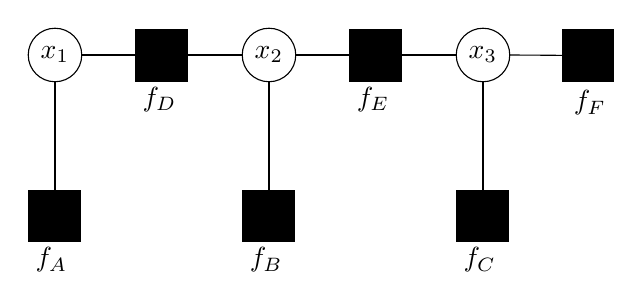
\begin{tikzpicture}[x=0.75pt,y=0.75pt,yscale=-1,xscale=1]
%uncomment if require: \path (0,288); %set diagram left start at 0, and has height of 288

%Shape: Square [id:dp542094098374186] 
\draw  [fill={rgb, 255:red, 0; green, 0; blue, 0 }  ,fill opacity=1 ] (86.34,228.71) -- (110.92,228.71) -- (110.92,253.29) -- (86.34,253.29) -- cycle ;
%Shape: Rectangle [id:dp9431678202688636] 
\draw  [fill={rgb, 255:red, 0; green, 0; blue, 0 }  ,fill opacity=1 ] (189.45,228.71) -- (214.03,228.71) -- (214.03,253.29) -- (189.45,253.29) -- cycle ;
%Shape: Rectangle [id:dp5515594438313509] 
\draw  [fill={rgb, 255:red, 0; green, 0; blue, 0 }  ,fill opacity=1 ] (292.57,228.71) -- (317.14,228.71) -- (317.14,253.29) -- (292.57,253.29) -- cycle ;
%Shape: Rectangle [id:dp19402149967725735] 
\draw  [fill={rgb, 255:red, 0; green, 0; blue, 0 }  ,fill opacity=1 ] (137.9,151.38) -- (162.47,151.38) -- (162.47,175.96) -- (137.9,175.96) -- cycle ;
%Shape: Rectangle [id:dp9723919948872586] 
\draw  [fill={rgb, 255:red, 0; green, 0; blue, 0 }  ,fill opacity=1 ] (241.01,151.38) -- (265.59,151.38) -- (265.59,175.96) -- (241.01,175.96) -- cycle ;
%Shape: Circle [id:dp9001944284946917] 
\draw   (86,163.41) .. controls (86,156.29) and (91.77,150.52) .. (98.89,150.52) .. controls (106.01,150.52) and (111.78,156.29) .. (111.78,163.41) .. controls (111.78,170.53) and (106.01,176.3) .. (98.89,176.3) .. controls (91.77,176.3) and (86,170.53) .. (86,163.41) -- cycle ;
%Shape: Ellipse [id:dp029985916423680425] 
\draw   (189.11,163.41) .. controls (189.11,156.29) and (194.88,150.52) .. (202,150.52) .. controls (209.12,150.52) and (214.89,156.29) .. (214.89,163.41) .. controls (214.89,170.53) and (209.12,176.3) .. (202,176.3) .. controls (194.88,176.3) and (189.11,170.53) .. (189.11,163.41) -- cycle ;
%Shape: Ellipse [id:dp8505763078012687] 
\draw   (292.22,163.41) .. controls (292.22,156.29) and (297.99,150.52) .. (305.11,150.52) .. controls (312.23,150.52) and (318,156.29) .. (318,163.41) .. controls (318,170.53) and (312.23,176.3) .. (305.11,176.3) .. controls (297.99,176.3) and (292.22,170.53) .. (292.22,163.41) -- cycle ;
%Straight Lines [id:da5591298719832298] 
\draw    (202,176.3) -- (202,236.1) ;
%Straight Lines [id:da8657801799701208] 
\draw    (305.11,176.3) -- (305.11,236.1) ;
%Straight Lines [id:da7323179142438296] 
\draw    (98.89,176.3) -- (98.89,236.1) ;
%Straight Lines [id:da2650402956705291] 
\draw    (141.85,163.41) -- (111.78,163.41) ;
%Straight Lines [id:da6929917679064295] 
\draw    (189.11,163.41) -- (159.04,163.41) ;
%Straight Lines [id:da7044874759875848] 
\draw    (244.96,163.41) -- (214.89,163.41) ;
%Straight Lines [id:da30371490539779855] 
\draw    (292.22,163.41) -- (262.15,163.41) ;
%Shape: Rectangle [id:dp26239558807935515] 
\draw  [fill={rgb, 255:red, 0; green, 0; blue, 0 }  ,fill opacity=1 ] (343.59,151.38) -- (368.16,151.38) -- (368.16,175.96) -- (343.59,175.96) -- cycle ;
%Straight Lines [id:da46629291479421253] 
\draw    (355.87,163.67) -- (318,163.41) ;


% Text Node
\draw (90.75,157.95) node [anchor=north west][inner sep=0.75pt]    {$x_{1}$};
% Text Node
\draw (193.86,157.95) node [anchor=north west][inner sep=0.75pt]    {$x_{2}$};
% Text Node
\draw (296.97,157.95) node [anchor=north west][inner sep=0.75pt]    {$x_{3}$};
% Text Node
\draw (88.3,255) node [anchor=north west][inner sep=0.75pt]    {$f_{A}$};
% Text Node
\draw (191.48,255) node [anchor=north west][inner sep=0.75pt]    {$f_{B}$};
% Text Node
\draw (294.53,255) node [anchor=north west][inner sep=0.75pt]    {$f_{C}$};
% Text Node
\draw (243.04,177.67) node [anchor=north west][inner sep=0.75pt]    {$f_{E}$};
% Text Node
\draw (139.79,177.67) node [anchor=north west][inner sep=0.75pt]    {$f_{D}$};
% Text Node
\draw (347.59,179.36) node [anchor=north west][inner sep=0.75pt]    {$f_{F}$};


\end{tikzpicture}


    \caption[Example factor graph]{An example of a factor graph}
\end{figure}

The above factor graph represents the following factorisation:

\begin{equation}
    p(X_1, X_2, X_3) = f_A(X_1)f_B(X_2)f_C(X_3)f_D(X_1, X_2)f_E(X_2, X_3)f_F(X_3)
    \label{eqn:factors}
\end{equation}

Assuming that each variable takes discrete values, suppose we wanted to find the probability that $X_1 = z$ for some value of $z$ using the above factor graph. Then we would need to find:

\begin{equation}
    p(X_1 = z, X_2, X_3) = \underset{i=X_2}{\sum} \underset{j=X_3}{\sum} p(X_1 = z, X_2 = i, X_3 =j)
    \label{eqn:bp_derivation_1}
\end{equation}

And by \ref{eqn:factors} we get:

\begin{equation}
    p(X_1 = z, X_2, X_3) = \underset{i=X_2}{\sum} \underset{j=X_3}{\sum} f_A(z)f_B(i)f_C(j)f_D(z, i)f_E(z, j)f_F(j)
\end{equation}


which can be rearranged to form:

\begin{equation}
    p(X_1 = z, X_2, X_3) = f_A(z) \underset{i=X_2}{\sum} \left(f_D(z, i)f_B(i) \left(\underset{j=X_3}{\sum} f_E(z, j)f_C(j)f_F(j) \right)\right)
    \label{eqn:x1}
\end{equation}

Similarly, if we wanted to find the probability that $X_2 = z$ for some z we would need to find:

\begin{equation}
    p(X_1, X_2 = z, X_3) = f_b(z) \left(\underset{i=X_1}{\sum} f_D(i, z) f_A(i)\right) \left(\underset{j=X_3}{\sum} f_E(z, j) f_C(j) f_F(j)\right)
    \label{eqn:x2}
\end{equation}

Noticing how the sum over $X_3$ in both \ref{eqn:x1} and \ref{eqn:x2} is the same, we may want to ``cache'' the result when dealing with large factor graphs, to improve performance. To do this we can associate calculations with nodes in the factor graph. We call these associations ``messages''.

The general form of a message from variable $i$ to factor $j$ is the product of the messages from all other neighbouring factors \cite{GaussianBP}. Formally:

\begin{equation}
    m_{x_i \rightarrow f_j} = \underset{s \in N(i) \backslash j }{\prod} m_{f_s \rightarrow x_i}
    \label{eqn:v_f}
\end{equation}

The general form of a message from factor $j$ to variable $i$ is the product of the messages from all other neighbouring variables and the factor applied to all other variables except $i$ \cite{GaussianBP}. Put formally:

\begin{equation}
    m_{f_j \rightarrow x_i} = \left(\underset{X_j \backslash x_i}{\sum} f_j(X_j)\right) \left(\underset{k \in N(j) \backslash i}{\prod} m_{x_k \rightarrow f_j}\right)
    \label{eqn:f_v}
\end{equation}

Finally, the marginal value (belief) of a variable is simply the product of all incoming messages to it \cite{GaussianBP}.

\begin{equation}
    p(x_i) = \underset{s \in N(i)}{\prod} m_{f_s \rightarrow x_i}
    \label{eqn:bp_belief}
\end{equation}

\subsection{Belief Propagation}
The above equations are used by the Belief Propagation algorithm, an iterative message-passing algorithm used to calculate the marginal value for each variable in a factor graph \cite{GaussianBP}. Each iteration of Belief Propagation has 3 phases:

\begin{enumerate}
    \item Variables send messages to each of their neighbouring factors \ref{eqn:v_f}.
    \item Factors send messages to each of their neighbouring variables \ref{eqn:f_v}.
    \item Each variable updates its ``belief'' (its estimated marginal value) \ref{eqn:bp_belief}.
\end{enumerate}

The original Belief Propagation algorithm was designed to be used in tree-like graphs, i.e. graphs without loops \cite{GaussianBP}. However, empirical evidence has shown that ``Loopy-BP'' can still converge to provide useful results in a variety of problem domains \cite{GaussianBP}. % TODO replace citations with better ones 

\subsection{Gaussian Belief Propagation}
A special case of the Belief Propagation algorithm is Gaussian Belief Propagation, which applies to problems where all variables follow a Gaussian distribution, and all factors are Gaussian functions of their inputs.

Under Gaussian Belief Propagation, each message can be interpreted as a Gaussian and so must contain sufficient information to produce one. A naive way of achieving this is to include a mean vector and a covariance matrix in each message. However, this approach is computationally expensive as it requires a full matrix multiplication whenever messages are multiplied which is an order $O(n^3)$ operation. An alternative approach is to use the \textit{canonical form} of the multivariate Gaussian distribution.

The canonical form uses an \textit{information vector} ($\eta$) and a \textit{precision matrix} ($\Lambda$) defined as follows:

\begin{align*}
    \eta = \Sigma^{-1} \mu && \Lambda = \Sigma^{-1}
\end{align*}

where $\Sigma$ is the covariance matrix and $\mu$ is the mean vector. Now multiplying messages is made more efficient as it only requires the addition of both messages' $\eta$ and $\Lambda$ values, making it an order $O(n^2)$ operation in the worst case. A further performance improvement can be made by recognising that the precision matrix is sparse \cite{GaussianBP}.

\unsure{Should I add equations for gbp?}

\subsection{Lie Theory}
Lie theory is a subset of group theory focussed on studying \textit{Lie groups}. Lie theory is a vast and abstract field, from which we only need to borrow a few concepts. The first is that positions and rotations can be represented as Lie groups, for example, the group $SO2$ represents a rotation in 2D space and the $SE3$ group represents a rigid motion in 3D space. The second core concept is the \textit{tangent space} which allows small deviations to be applied to the Lie group uniformly regardless of the value it operates on. This concludes our whirlwind tour of Lie theory, we invite the reader to read \cite{MicroLieTheory} for a more detailed tutorial.

% QUESTION: Do I need this at all?
% A group is a set of elements $G$ combined with a composition operation $\circ$, such that the following properties hold:
% \begin{enumerate}
%     \item Composing 2 elements of G results in another element of G
%     \item There exists an identity element $\epsilon$ so that composing any element with $\epsilon$ or $\epsilon$ with any element results in the same element
%     \item Composing an element with its inverse results in $\epsilon$
%     \item Composition is associative
% \end{enumerate}

% A Lie group is a group combined with a smooth manifold

\subsection{Putting it all together}
Now that we have covered all of the prerequisites to understanding how the Robot Web operates, we shall now demonstrate how they can be assembled into the Robot Web.

Every robot in the Robot Web needs to estimate its current location at all times, this is called localisation. One simple localisation method is to use odometry, which uses internal sensors to measure its displacement from its previous location. Since no sensor is perfect, this introduces a small amount of noise, which can be accurately modelled using a Gaussian distribution. The Robot Web simulates odometry using a factor graph, each known position of the robot maps to a pose variable, and the variables of each pair of successive positions are connected by an odometry factor. On every timestep, the robot performs an iteration of Gaussian Belief Propagation to estimate its current position.

The Robot Web further improves the accuracy of robots' locations by allowing robots to measure each other using external sensors. When a robot senses another, it creates a factor in its factor graph between its and the other's latest pose variables. When each robot wants to send a message to another, it publishes the message to its \textbf{Robot Web Page}, which the other robot will eventually read and use to update its location estimate.

\begin{figure}[!h]
    \centering
    

\tikzset{every picture/.style={line width=0.75pt}} %set default line width to 0.75pt        

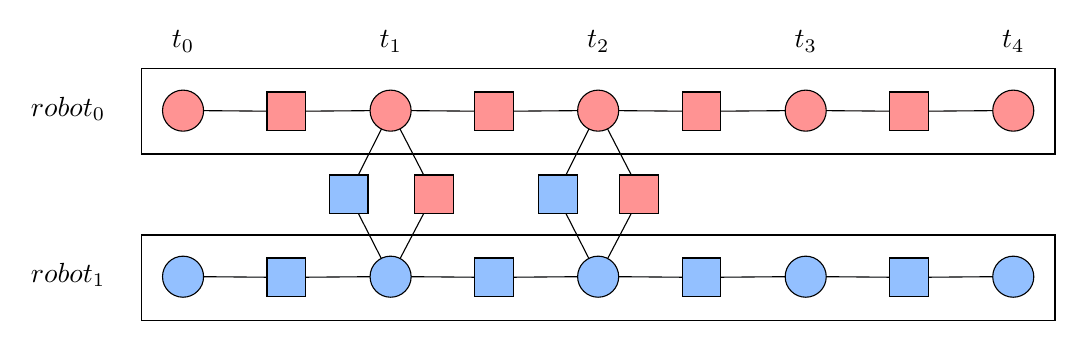
\begin{tikzpicture}[x=0.75pt,y=0.75pt,yscale=-1,xscale=1]
%uncomment if require: \path (0,288); %set diagram left start at 0, and has height of 288

%Straight Lines [id:da47036734988196627] 
\draw    (299.67,170.04) -- (319.89,209.71) ;
%Straight Lines [id:da6881382794521629] 
\draw    (319.89,129.71) -- (299.67,170.04) ;
%Straight Lines [id:da3959117741800886] 
\draw    (319.89,129.71) -- (340.67,170.04) ;
%Straight Lines [id:da6282284807536171] 
\draw    (340.67,170.04) -- (319.89,209.71) ;
%Straight Lines [id:da5198960712037324] 
\draw    (199.67,170.04) -- (219.89,209.71) ;
%Straight Lines [id:da8902598554725618] 
\draw    (219.89,129.71) -- (199.67,170.04) ;
%Straight Lines [id:da2738660568678817] 
\draw    (219.89,129.71) -- (240.67,170.04) ;
%Straight Lines [id:da06728554169051759] 
\draw    (240.67,170.04) -- (219.89,209.71) ;
%Straight Lines [id:da34036055728120096] 
\draw [fill={rgb, 255:red, 255; green, 147; blue, 147 }  ,fill opacity=1 ]   (329.78,129.71) -- (369.67,130.04) ;
%Straight Lines [id:da8072322510197338] 
\draw [fill={rgb, 255:red, 255; green, 147; blue, 147 }  ,fill opacity=1 ]   (369.67,130.04) -- (410,129.71) ;
%Straight Lines [id:da405451058550087] 
\draw [fill={rgb, 255:red, 255; green, 147; blue, 147 }  ,fill opacity=1 ]   (429.78,129.71) -- (469.67,130.04) ;
%Straight Lines [id:da7616794610228106] 
\draw [fill={rgb, 255:red, 255; green, 147; blue, 147 }  ,fill opacity=1 ]   (469.67,130.04) -- (510,129.71) ;
%Straight Lines [id:da6814419083610201] 
\draw [fill={rgb, 255:red, 255; green, 147; blue, 147 }  ,fill opacity=1 ]   (229.78,129.71) -- (269.67,130.04) ;
%Straight Lines [id:da7724102331322766] 
\draw [fill={rgb, 255:red, 255; green, 147; blue, 147 }  ,fill opacity=1 ]   (269.67,130.04) -- (310,129.71) ;
%Straight Lines [id:da5821529621200299] 
\draw [fill={rgb, 255:red, 255; green, 147; blue, 147 }  ,fill opacity=1 ]   (169.67,130.04) -- (210,129.71) ;
%Straight Lines [id:da0542087989667579] 
\draw [fill={rgb, 255:red, 255; green, 147; blue, 147 }  ,fill opacity=1 ]   (129.78,129.71) -- (169.67,130.04) ;
%Shape: Square [id:dp4499442483222458] 
\draw  [fill={rgb, 255:red, 255; green, 147; blue, 147 }  ,fill opacity=1 ] (160.34,120.71) -- (179,120.71) -- (179,139.37) -- (160.34,139.37) -- cycle ;
%Shape: Circle [id:dp2600881142320077] 
\draw  [fill={rgb, 255:red, 255; green, 147; blue, 147 }  ,fill opacity=1 ] (110,129.71) .. controls (110,124.25) and (114.43,119.82) .. (119.89,119.82) .. controls (125.35,119.82) and (129.78,124.25) .. (129.78,129.71) .. controls (129.78,135.17) and (125.35,139.6) .. (119.89,139.6) .. controls (114.43,139.6) and (110,135.17) .. (110,129.71) -- cycle ;
%Shape: Rectangle [id:dp7305091073359651] 
\draw   (100,109.6) -- (540,109.6) -- (540,150.6) -- (100,150.6) -- cycle ;
%Shape: Square [id:dp49665350033925293] 
\draw  [fill={rgb, 255:red, 255; green, 147; blue, 147 }  ,fill opacity=1 ] (260.34,120.71) -- (279,120.71) -- (279,139.37) -- (260.34,139.37) -- cycle ;
%Shape: Circle [id:dp8551402235390253] 
\draw  [fill={rgb, 255:red, 255; green, 147; blue, 147 }  ,fill opacity=1 ] (210,129.71) .. controls (210,124.25) and (214.43,119.82) .. (219.89,119.82) .. controls (225.35,119.82) and (229.78,124.25) .. (229.78,129.71) .. controls (229.78,135.17) and (225.35,139.6) .. (219.89,139.6) .. controls (214.43,139.6) and (210,135.17) .. (210,129.71) -- cycle ;
%Shape: Square [id:dp6259568957324568] 
\draw  [fill={rgb, 255:red, 255; green, 147; blue, 147 }  ,fill opacity=1 ] (360.34,120.71) -- (379,120.71) -- (379,139.37) -- (360.34,139.37) -- cycle ;
%Shape: Circle [id:dp7516686593765485] 
\draw  [fill={rgb, 255:red, 255; green, 147; blue, 147 }  ,fill opacity=1 ] (310,129.71) .. controls (310,124.25) and (314.43,119.82) .. (319.89,119.82) .. controls (325.35,119.82) and (329.78,124.25) .. (329.78,129.71) .. controls (329.78,135.17) and (325.35,139.6) .. (319.89,139.6) .. controls (314.43,139.6) and (310,135.17) .. (310,129.71) -- cycle ;
%Shape: Square [id:dp4907257696393781] 
\draw  [fill={rgb, 255:red, 255; green, 147; blue, 147 }  ,fill opacity=1 ] (460.34,120.71) -- (479,120.71) -- (479,139.37) -- (460.34,139.37) -- cycle ;
%Shape: Circle [id:dp40511868636697557] 
\draw  [fill={rgb, 255:red, 255; green, 147; blue, 147 }  ,fill opacity=1 ] (410,129.71) .. controls (410,124.25) and (414.43,119.82) .. (419.89,119.82) .. controls (425.35,119.82) and (429.78,124.25) .. (429.78,129.71) .. controls (429.78,135.17) and (425.35,139.6) .. (419.89,139.6) .. controls (414.43,139.6) and (410,135.17) .. (410,129.71) -- cycle ;
%Shape: Circle [id:dp7561415264055935] 
\draw  [fill={rgb, 255:red, 255; green, 147; blue, 147 }  ,fill opacity=1 ] (510,129.71) .. controls (510,124.25) and (514.43,119.82) .. (519.89,119.82) .. controls (525.35,119.82) and (529.78,124.25) .. (529.78,129.71) .. controls (529.78,135.17) and (525.35,139.6) .. (519.89,139.6) .. controls (514.43,139.6) and (510,135.17) .. (510,129.71) -- cycle ;
%Straight Lines [id:da6629990224165134] 
\draw [fill={rgb, 255:red, 147; green, 192; blue, 255 }  ,fill opacity=1 ]   (329.78,209.71) -- (369.67,210.04) ;
%Straight Lines [id:da6819695700249584] 
\draw [fill={rgb, 255:red, 147; green, 192; blue, 255 }  ,fill opacity=1 ]   (369.67,210.04) -- (410,209.71) ;
%Straight Lines [id:da7961157322315353] 
\draw [fill={rgb, 255:red, 147; green, 192; blue, 255 }  ,fill opacity=1 ]   (429.78,209.71) -- (469.67,210.04) ;
%Straight Lines [id:da7688161886956275] 
\draw [fill={rgb, 255:red, 147; green, 192; blue, 255 }  ,fill opacity=1 ]   (469.67,210.04) -- (510,209.71) ;
%Straight Lines [id:da8267819717164204] 
\draw [fill={rgb, 255:red, 147; green, 192; blue, 255 }  ,fill opacity=1 ]   (229.78,209.71) -- (269.67,210.04) ;
%Straight Lines [id:da5116263132351999] 
\draw [fill={rgb, 255:red, 147; green, 192; blue, 255 }  ,fill opacity=1 ]   (269.67,210.04) -- (310,209.71) ;
%Straight Lines [id:da7065942165163066] 
\draw [fill={rgb, 255:red, 147; green, 192; blue, 255 }  ,fill opacity=1 ]   (169.67,210.04) -- (210,209.71) ;
%Straight Lines [id:da6801634542744135] 
\draw [fill={rgb, 255:red, 147; green, 192; blue, 255 }  ,fill opacity=1 ]   (129.78,209.71) -- (169.67,210.04) ;
%Shape: Square [id:dp5838901472847389] 
\draw  [fill={rgb, 255:red, 147; green, 192; blue, 255 }  ,fill opacity=1 ] (160.34,200.71) -- (179,200.71) -- (179,219.37) -- (160.34,219.37) -- cycle ;
%Shape: Circle [id:dp8237018481465868] 
\draw  [fill={rgb, 255:red, 147; green, 192; blue, 255 }  ,fill opacity=1 ] (110,209.71) .. controls (110,204.25) and (114.43,199.82) .. (119.89,199.82) .. controls (125.35,199.82) and (129.78,204.25) .. (129.78,209.71) .. controls (129.78,215.17) and (125.35,219.6) .. (119.89,219.6) .. controls (114.43,219.6) and (110,215.17) .. (110,209.71) -- cycle ;
%Shape: Rectangle [id:dp1468154649235054] 
\draw   (100,189.6) -- (540,189.6) -- (540,230.6) -- (100,230.6) -- cycle ;
%Shape: Square [id:dp21555253881823844] 
\draw  [fill={rgb, 255:red, 147; green, 192; blue, 255 }  ,fill opacity=1 ] (260.34,200.71) -- (279,200.71) -- (279,219.37) -- (260.34,219.37) -- cycle ;
%Shape: Circle [id:dp8554188945699046] 
\draw  [fill={rgb, 255:red, 147; green, 192; blue, 255 }  ,fill opacity=1 ] (210,209.71) .. controls (210,204.25) and (214.43,199.82) .. (219.89,199.82) .. controls (225.35,199.82) and (229.78,204.25) .. (229.78,209.71) .. controls (229.78,215.17) and (225.35,219.6) .. (219.89,219.6) .. controls (214.43,219.6) and (210,215.17) .. (210,209.71) -- cycle ;
%Shape: Square [id:dp5941665721073983] 
\draw  [fill={rgb, 255:red, 147; green, 192; blue, 255 }  ,fill opacity=1 ] (360.34,200.71) -- (379,200.71) -- (379,219.37) -- (360.34,219.37) -- cycle ;
%Shape: Circle [id:dp5825532487467875] 
\draw  [fill={rgb, 255:red, 147; green, 192; blue, 255 }  ,fill opacity=1 ] (310,209.71) .. controls (310,204.25) and (314.43,199.82) .. (319.89,199.82) .. controls (325.35,199.82) and (329.78,204.25) .. (329.78,209.71) .. controls (329.78,215.17) and (325.35,219.6) .. (319.89,219.6) .. controls (314.43,219.6) and (310,215.17) .. (310,209.71) -- cycle ;
%Shape: Square [id:dp7753119223119171] 
\draw  [fill={rgb, 255:red, 147; green, 192; blue, 255 }  ,fill opacity=1 ] (460.34,200.71) -- (479,200.71) -- (479,219.37) -- (460.34,219.37) -- cycle ;
%Shape: Circle [id:dp5771019164898812] 
\draw  [fill={rgb, 255:red, 147; green, 192; blue, 255 }  ,fill opacity=1 ] (410,209.71) .. controls (410,204.25) and (414.43,199.82) .. (419.89,199.82) .. controls (425.35,199.82) and (429.78,204.25) .. (429.78,209.71) .. controls (429.78,215.17) and (425.35,219.6) .. (419.89,219.6) .. controls (414.43,219.6) and (410,215.17) .. (410,209.71) -- cycle ;
%Shape: Circle [id:dp21210412845989923] 
\draw  [fill={rgb, 255:red, 147; green, 192; blue, 255 }  ,fill opacity=1 ] (510,209.71) .. controls (510,204.25) and (514.43,199.82) .. (519.89,199.82) .. controls (525.35,199.82) and (529.78,204.25) .. (529.78,209.71) .. controls (529.78,215.17) and (525.35,219.6) .. (519.89,219.6) .. controls (514.43,219.6) and (510,215.17) .. (510,209.71) -- cycle ;
%Shape: Square [id:dp7557733799934572] 
\draw  [fill={rgb, 255:red, 147; green, 192; blue, 255 }  ,fill opacity=1 ] (190.34,160.71) -- (209,160.71) -- (209,179.37) -- (190.34,179.37) -- cycle ;
%Shape: Square [id:dp8894509337156504] 
\draw  [fill={rgb, 255:red, 255; green, 147; blue, 147 }  ,fill opacity=1 ] (231.34,160.71) -- (250,160.71) -- (250,179.37) -- (231.34,179.37) -- cycle ;
%Shape: Square [id:dp6301411170449531] 
\draw  [fill={rgb, 255:red, 255; green, 147; blue, 147 }  ,fill opacity=1 ] (330.34,160.71) -- (349,160.71) -- (349,179.37) -- (330.34,179.37) -- cycle ;
%Shape: Square [id:dp8001210630138842] 
\draw  [fill={rgb, 255:red, 147; green, 192; blue, 255 }  ,fill opacity=1 ] (291.34,160.71) -- (310,160.71) -- (310,179.37) -- (291.34,179.37) -- cycle ;

% Text Node
\draw (113.3,90) node [anchor=north west][inner sep=0.75pt]    {$t_{0}$};
% Text Node
\draw (213.3,90) node [anchor=north west][inner sep=0.75pt]    {$t_{1}$};
% Text Node
\draw (313.3,90) node [anchor=north west][inner sep=0.75pt]    {$t_{2}$};
% Text Node
\draw (413.3,90) node [anchor=north west][inner sep=0.75pt]    {$t_{3}$};
% Text Node
\draw (513.3,90) node [anchor=north west][inner sep=0.75pt]    {$t_{4}$};
% Text Node
\draw (45.3,122) node [anchor=north west][inner sep=0.75pt]    {$robot_{0}$};
% Text Node
\draw (45.3,202) node [anchor=north west][inner sep=0.75pt]    {$robot_{1}$};


\end{tikzpicture}

    \caption[Robot Web factor graph]{An example of a factor graph in the Robot Web. Each robot's variables are connected by odometry factors. At times $t_1$ and $t_2$, both robots sense each other, and so exchange measurements by creating inter-robot-measurement factors on the graph.}
\end{figure}

%TODO - the real reason for lie groups is to nicely apply gaussians
The Robot Web represents the locations and sensor measurements of all robots using general Lie groups, rather than any specific group. This has the consequence that any type of sensor or robot can be a part of the Robot Web. For example, a drone moving in 3D space can interact with a car moving on a plane.

\subsection{Evaluation}
The Robot Web has been shown to improve the accuracy of robot localisation, and most importantly the inter-robot measurements have been shown to provide further improvements over schemes where robots would only measure landmarks. % TODO citation needed?

Furthermore, the Robot Web has proven to be robust to a large number of faulty inter-robot sensors reporting random measurements, with this robustness lasting until 70-80\% of inter-robot sensors reported corrupted measurements.

\begin{figure}[!h]
    \centering
    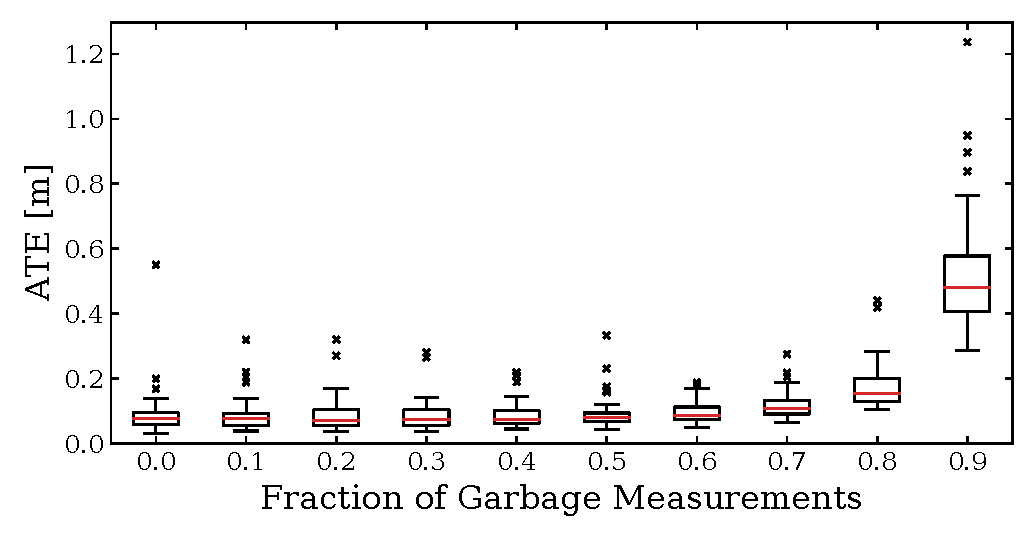
\includegraphics[page=1,width=.60\textwidth]{diagrams/sensor_noise.pdf}
    \caption[RobotWeb's robustness to garbage measurements]{A graph showing that the RobotWeb is robust to up to 70-80\% of ``garbage'' measurements, where faulty sensors report random measurements. ATE refers to the average Absolute Trajectory Error measured over 50 runs in an environment with 50 robots and 10 beacons running for 100 timesteps. Taken from \cite[Figure~5]{Robotweb}}
\end{figure}

Although the Robot Web is robust to many inter-robot sensors reporting random measurements, it is not robust to a bad actor which may instead report incorrect measurements designed to worsen the localisation of other members of the Robot Web. Possible attacks include but are not limited to:

\begin{enumerate}
    \item Sending messages with extremely high confidences, to lull others into a false sense of security.
    \item Sending these messages whilst assuming the identity of another robot.
    \item Sending these messages from many nonexistent robots, also known as a Sybil attack.
\end{enumerate}

\section{Security Issues}
In this section, we will discuss several general security issues that can arise in robot networks. We will focus on issues that affect the accuracy of a robot's internal model of the world. This excludes attacks which may result in an attacker gaining control over a robot, yet includes attacks performed by hijacked robots.

\subsection{Denial of Service} % Can go into more detail if necessary.
A denial of service attack seeks to deny service. In a robot network such as the Robot Web, this would prevent one or more robots from being able to access messages sent by their peers and essentially cut them off from the network.

The simplest way for an attacker to perform a DoS attack is to use a signal jammer, which can be constructed using off-the-shelf equipment \cite{SignalJamming}. This would continuously transmit signals within the range of frequencies allowed by the communication medium, both interfering with and irrecoverably corrupting any messages sent. More sophisticated attackers may craft harder-to-detect jammer attacks by mimicking legitimate messages or only transmitting when it senses communication \cite{SignalJamming}. In addition to these, there exist a whole host of jamming attacks (and defences) targetting specific communication protocols.

Another form of a DoS attack would be to disconnect specific robots from the network, using the network protocol's existing defences. For example, by convincing others that the target is a bad actor, triggering their defences to remove the target from the network. % Kinda like a de-authentication attack, but not really since we're not sending explicit de-authentication frames to do this.

\subsection{Identity-Based Attacks}
% One class of attacks that could wreak havoc on robot networks are identity-based attacks; here a nonzero number of bad actors, claim false identities, which may or may not correspond to other robots in the network. The former is known as a spoofing attack, whilst the latter constitutes a Sybil attack.

Identity-based attacks can wreak havoc on robot networks. Using the model defined by Douceur \cite{SybilAttack}, we can describe a robot network as one consisting of $E$ entities (robots) each claiming at least one identity $i$ from the set of all identities $I$. When the network is under an identity-based attack, at least one of the following two properties will hold: % TODO maybe add the faulty/correct distinction
\begin{enumerate}
    \item Two entities, $e1, e2$ will present the same identity $i$
    \item The number of identities in $I$ will exceed the number of entities in $E$.
\end{enumerate}
If only the former holds, then the network is under a spoofing attack, whereas if only the latter holds, then the network is under a Sybil attack. Note: there is no guarantee that only one of these will hold at a time, and so we must be prepared to defend against both simultaneously.

\subsubsection{Spoofing Attacks}
Devices exchange information by sending packets or frames of data. For our purposes, we can ignore the differences between packets and frames, and use the terms interchangeably. Packets are used to encapsulate the data sent with relevant metadata, such as the source and destination IDs of the packet. This metadata is the main target of spoofing attacks.

In a spoofing attack, the attacker first finds the identity of a legitimate device, for example by first intercepting packets and then extracting the source ID from them. After this point, the attacker sends misleading packets impersonating the target. 

This can have several benefits for the attacker. Firstly, they could covertly inject misinformation into the network by impersonating an already trusted robot. Secondly, they could trigger defences in the network to flag target for misinformation and remove it.

\subsubsection{Sybil Attacks}
In a Sybil attack, the attacker will create many fake identities to gain undue influence on the network. In a robot network, this would allow them to indirectly influence the actions of victim robots. For example, one could lead two self-driving cars to conclude that their best course of action is to crash, by claiming many false identities would be hit if they were not to.

Douceur \cite{SybilAttack} proves Sybil attacks are always possible in distributed systems where there is no central arbiter of truth. They present and prove four lemmas about identities in large-scale distributed systems. The first two lemmas are concerned with entities which directly validate the identities presented to them, whilst the second two lemmas involve entities which rely upon other, potentially untrustworthy, identities for validation. The lemmas are as follows:

 %TODO lemma-ise

\begin{enumerate}
    \item If an attacker has $\rho$ times as many resources as the weakest entity, then they can successfully present up to $\lfloor\rho\rfloor$ distinct identities.
    \item If an entity doesn't validate all identities simultaneously, then an attacker can present an unbounded number of distinct identities.
    \item If an entity trusts $q$ other identities to validate an identity, then at least $f$ attackers are required to perform the attack, where $f >= q$ or the resources commanded by the attackers exceed $q + f$ times the weakest entity's resources.
    \item If all $c$ non-attackers don't coordinate when they validate identities, and an entity again trusts $q$ other identities for validation, then even a weak attacker can present $\lfloor\frac{c}{q}\rfloor$ identities.
\end{enumerate}

We plan to solve this problem by treating the physical world as a central arbiter of truth, albeit with some degree of error, due to imperfections in sensors.

\subsection{Physical Attacks}
Finally, since this thesis focuses on the security of robot networks, we will discuss the possibility of physical attacks on the system, and our limited ability to protect against them. We define a physical attack as any attempt to compromise the ability of a robot to perform its task. This includes colliding with the robot but also includes more subtle tactics, such as obscuring the robot's sensors. Physical attacks could also be used similarly to Sybil attacks, where several attackers would surround a robot and feed it misinformation. 

In this thesis, we will not attempt to protect against attacks where several robots would physically collide, since this would require heavy hardware modifications to existing robots. Instead, we will focus on occlusion attacks and physical Sybil attacks, at the very least allowing a robot to detect them.\\
% \chapter{Related Work}
\noindent\makebox[\linewidth]{\rule{\textwidth}{1pt}}


Several different techniques have been explored in preventing the types of identity-based attacks discussed in this chapter. In the \nth{2} half of this chapter, we will examine and evaluate these. We broadly group these approaches into 2 main groups; the first uses the physical characteristics of signal propagation to bind an identity to an entity, whilst the second exploits the fact that no entity can perform an unlimited amount of computation.

\section{Wifi Fingerprinting}
% In this section, we will review two Wifi fingerprinting-based approaches to binding identities to entities. 

There are many ways for devices to communicate wirelessly, many of which use radiowaves. Wifi is the name of a family of networking protocols that allow for this, it derives from the IEEE 802.11 standard. In order to use Wifi, a device must have at least one wireless antenna which can transmit and receive within the bands specified in the IEEE 802.11 standard; usually 2.4GHz and 5GHz.

When a device sends a packet using Wifi, it transmits a radio signal for a given number of nanoseconds from its antenna. This signal will attenuate as it travels further and further through space. After a certain distance, also known as the communicating range of the antenna, the signal will fade into background noise. The signal leaves the antenna in all directions simultaneously, as a radio wave. Eventually, a small part of this wave will reach the receiver's antenna and the packet will be decoded out of it.

Other parts of the wave will either diffract around corners, reflect off some large objects, or scatter off many small objects \cite{SignalProp}. Consequently, this means that a receiver may receive a packet from several different directions simultaneously, that is that it could encounter different parts of the same wave from different directions at the same time. This phenomenon is known as multipath scattering. %TODO Add diagram? 

Multipath scattering has two interesting properties; it is practically impossible to predict, ahead of time, the distribution of signals around a receiver and it is unlikely that two receivers will observe the same signal propagation with sufficient multipath scattering\citationneeded. These properties allow for devices to ``fingerprint'' every packet they receive, such that two different transmitters cannot have the same fingerprint unless they are simultaneously located at the same place. 

However, implementing multipath scattering-based algorithms have some technical constraints; namely that the receiving antenna must be able to measure the signal in each direction, and that a sufficient amount of multipath scattering must occur. Usually, these algorithms struggle in outdoor environments, where the environment may not provide objects for multipath scattering to occur\citationneeded.

The following papers discuss methods to circumvent these constraints, focussing on securing robot networks from spoofing and Sybil attacks. 

\subsection{Guaranteeing spoof-resilient multi-robot networks}
Gil et al, \cite{GuaranteeingSpoofResilience} provides an interesting approach to some of the aforementioned problems, most notably the problem of requiring expensive hardware to allow the receiving antenna to measure the signal in each direction. They do this by inventing an algorithm that allows them to build a ``virtual spoofer sensor'' only using commercially available wifi hardware, which creates a ``spatial fingerprint'' from each transmission in the network. They use the output from this sensor to calculate a confidence metric $\alpha$ indicating their algorithm's confidence that a robot's identity is its entity. Finally, they characterise the theoretical performance of the ``virtual spoofer sensor'' and provide empirical evidence to support their claims by undertaking several experiments.

The authors build the ``virtual spoofer sensor'' by building upon \textit{Synthetic Aperture Radar} (SAR) techniques, which allow a single antenna to be used to simulate an antenna array. SAR involves moving the antenna to different locations and taking snapshots of the signals received. These snapshots are then combined using signal-processing techniques to emulate a multi-antenna array \cite{BAD_SAR}.\unsure{Diagram needed?}
%TODO: This isn't a great citation, go to the original paper
The ``spatial fingerprint'' calculated, is then compared to the fingerprints of other clients, and clients with identical fingerprints are assumed to be Sybil attackers.

The authors evaluate their algorithm in the context of the following problem statement. Given an environment with several ``clients'', each expecting service from mobile ``servers'', dynamically find the optimal layout for the servers such that each ``client'' is served. A subset of clients are assumed to be malicious and are carrying out Sybil attacks in order to influence the ``servers'' to move closer to them.

The authors perform four experiments to validate their hypotheses:
\begin{enumerate}
    \item They compare the performance of the ``virtual spoofer sensor'' in both an indoor and simulated outdoor environment, as expected, finding that multipath scattering is more effective in indoor settings, but also that adding a single reflector to the environment vastly improves performance.
    \item They compare the effect of a stationary, moving, and power-scaling Sybil attacker on the ability of the ``virtual spoofer sensor'' to correctly classify agents, resulting in no false negatives, but many false positives.
    \item They evaluate their system on the multi-agent coverage problem \cite{MultiAgentCoverage}, finding that it can provide near-optimal results even when there are 3$\times$ more spoofed agents.
    \item They apply their system to a drone delivery problem, where the ``server'' needs to visit each real ``client'' to deliver a package and again find that their system provides near-optimal results when there are 3$\times$ more spoofed agents.
\end{enumerate}

\unsure{I have suspicions about how they did the last 2 experiments, especially since the phantoms are nowhere near the actual attacker.}

\subsection{Lightweight Sybil-Resilient Multi-Robot Networks by Multipath Manipulation}
Huang et al. \cite{MultiPathManipulation} take a different approach to Gil et al. \cite{GuaranteeingSpoofResilience}; instead of relying upon the environment to provide multipath scattering, they actively cause it by using backscatter tags. This offers two main advantages over Gil et al.: \begin{enumerate*}
    \item the environment has a lesser effect on the performance of the Sybil attack detector and
    \item the robots' antennae no longer need to move when capturing a fingerprint.
\end{enumerate*}
Using the captured signal information, the robots again compute a fingerprint per transmission, normalise it to mitigate the effects of any power scaling attacks, and finally compare the normalised fingerprint to those of all others, treating any identities with sufficiently similar fingerprints as Sybil attackers.

Backscatter tags scatter signals that they encounter by rapidly absorbing and reflecting them. Backscatter tags also simplify the fingerprinting process, since robots are no longer required to perform small movements for SAR, nor must the software engage in expensive linear algebra to construct a multi-antenna array. 

A key property of backscatter tags is that they operate passively and don't require a power supply. This reduces the cost of implementing this scheme as tags can be simply and inexpensively attached to robots. Another useful property is that the backscattering of the final signal is highly correlated with the positions of the tags, transmitting and receiving antennae, meaning that if two identities have very similar backscattering patterns, they are likely to originate from the same entity.

When a robot receives a signal, it receives a raw signal, which is first smoothed out with a moving average filter, to create the backscattered signal. Then it decodes a message out of the backscattered signal, and uses it, with signal processing techniques to deduce how much each tag contributed to the backscattering, and when each tag was ``activated''. Then the robot does more filtering to remove any backscattering from the environment, the resulting signal will be used to construct a signature for the transmission.

The authors then evaluate their implementation in both an indoor office environment and an outdoor rooftop environment. They find that their method is virtually indifferent to the surrounding environment, as they measure an average true positive rate of 97.6\% and an average false positive rate of 5.1\%.

\subsection{Conclusions}

Although both sets of authors extensively test their system, they make some problematic assumptions, which may be exploited by attackers. 

\begin{enumerate}
    \item They do not account for Sybil attacks using multiple antennae, which could transmit the same message at the same time, but with variable power levels. Each antenna would create a different multipath scatter, and if the relative powers between them were varied, then they could theoretically construct many false fingerprints.
    \item They also do not account for collaboration between different attackers, which would function similarly to the previous vulnerability, where geographically distributed attackers could simultaneously send the same message, with different power scales, creating another set of false fingerprints. This method could produce a larger range of false identities but may encounter synchronisation problems between attackers.
    \item Attackers could leverage methods similar to Huang et al. and physically augment their antennae to manipulate their multipath scattering, for example, one could create moveable barriers to prevent some scattering from occurring.
    \item Both sets of authors assume that any noise from the environment will not be malicious; Gil et al. assume that it will follow a Gaussian distribution, whilst Huang et al. assume that standard signal processing techniques would be sufficient to filter it out. Both of these assumptions fail to account for the possibility that coordinated attackers emit noise above background levels, but not so high that it would seriously interfere with transmissions. This would disrupt every transmission's signature and would prevent any pair of transmissions from looking alike.
\end{enumerate}


% \todo{Add diagram for 3}

\section{Proof of Work}
Proof of Work is underpinned by the insight that no entity in a network can perform unlimited computation. This leads to defences reliant on the idea that generating identities should be computationally expensive, to prevent any entity from being able to create an unbounded number of them. A PoW identity generation scheme would express an identity as the solution to some puzzle, and thus the identity can be validated by checking if it is a valid solution to the puzzle. This imposes two constraints: \begin{enumerate*}
    \item the puzzle must be hard to solve and
    \item the solution to a puzzle must be easy to verify
\end{enumerate*}, which means that, formally, the puzzle belongs to the \textit{NP-Complete} class of problems.

A problem with this strategy is that it requires wasting computational resources, which may be in short supply for the embedded systems used in robotics. Furthermore, it requires that normal robots constantly pay a steep price for their security even without the presence of attackers.

Gupta et al. \cite{PoW} design an iterative algorithm (\textbf{GMCom}) that solves the \nthM{2} problem, where if attackers spend $T$ resources, whilst $J$ new non-attacking identities are presented, then each non-attacker only needs to spend $O(\sqrt[2]{TJ} + J)$ resources. They refer to this property as the \textit{assymetry} of the algorithm, as attackers must spend many more resources than non-attackers.

GMCom organises identities into a group, where a subset of them form a committee. When a new identity tries to join the group, it must first solve a puzzle set by the committee. Occasionally, the committee will seek to purge all attackers from the group, by issuing a \textit{purge puzzle}, which must be solved by all identities before a new committee is formed, otherwise the identity will be purged from the group. This limits the wasted computation that good entities must perform since they only need to solve a single puzzle when entering a group, and occasionally thereafter, whilst an attacker would need to solve puzzles for each identity it claims, and would need to solve them repeatedly to avoid being purged.

However, this approach is not without its limitations. The authors assume that attackers will always only be able to command a fraction, $\alpha$, of the total resources of the system, however, the heterogeneous nature of robots means that this may not always be guaranteed. For example, in a drone delivery system, each drone would likely only possess a small amount of computational power, but an attacker may attack the system using their desktop computer.

% GMCom organises identities into a group, where a subset of them form a committee. When a new identity tries to join the group, it must first solve a current epoch's puzzle, set by the committee, and broadcast its solution. Once a certain number of identities has joined or left the group, the committee starts the next epoch with a new puzzle and new committee. 
% \section{Attacks on sensor networks}
% \section{Reputation based systems}

\chapter{An Investigation into the Security of RobotWeb}
This chapter will investigate the behaviour of the RobotWeb when it is under attack. We will start by definining the expected behaviour of an attacker, including its incentives to attack. From then, we will construct and examine a simplified version of the RobotWeb to determine how victims of an attack will behave. Finally, we present and test several hypotheses about the behaviour of the RobotWeb under attack.

\section{The behaviour of an ideal attacker}
In order to predict the nature of an attacker's behaviour, we must first understand how normal robots behave in the RobotWeb. At all times, a robot will have a noisy estimate of its current position, as it moves the associated noise will grow. When robot $r_1$ encounters another $r_2$, it measures it and creates a factor between its own and $r_2$'s current pose variable. Both robots will then exchange messages to each other over the factor, both using the messages to improve their own location estimates and decrease their uncertainty. In addition to other robots, a robot may measure a fixed beacon, which once again creates a factor between them, however, here only the robot will update its position estimate, as the beacon does not move. The quality of all sent message is dependent on the sender's own position accuracy and the accuracy of its sensors.

An attacker can take the form of either another robot or a beacon in the RobotWeb. Regardless of the form taken by the attacker, its goal would be to control the other robots' position estimates, by sending specially crafted messages.

All robots require a method to localise themselves as part of their normal operations, even attackers. Normal robots use the RobotWeb to do this, while we have no guarantees on the methods that potential attackers may use. An attacker may use an external system for localisation, or even a private RobotWeb, which renders it impervious to any consequences for its actions. However, some attackers may instead choose to participate in the RobotWeb in order to avoid the complexity of using an alternative system. Participating attackers would then have incentive to partially preserve the RobotWeb as they themselves are dependent on it. This dependency is likely cause attackers to only attack a small subset of robots, or only attack robots for a small amount of time. 

It is self-evident that all attackers would seek to be effective i.e. thier attacks should have a high chance of working especially when no defences are present. In seeking effectiveness in the face of defences, attackers should not want their attacks to be easily identified, as identified attacks can be easily defended against. Thus it stands to reason that attacks are likely to be subtly executed, such that their victims would be able to believe them. For example, an attack that suggests that a small robot has moved 10km in 5s is guaranteed to fail.

Finally, in the event that multiple attackers are present in the environment, they would do best to collaborate rather than compete, as it would raise the effectiveness of them all. Since competing attackers are less effective than collaborating attackers, we shall spend less time considering them.

\section{A simplified system}
Any theoretical investigation of the RobotWeb would require the investigator to analyse its backbone, the factor graph. However, the investigator would soon find themselves ensnared by complexity; caught in an intricate web of variable and factor nodes; messages constantly scurrying between them. Worse yet, the web would constantly be spun and unspun as robots moved closer and further from each other.
In the face of this complexity, it becomes clear that a simplification is needed.

To start, we choose to limit our investigation to a single variable, chosen arbitrarily, in the factor graph. Fortunately, the properties of Belief Propagation allow us to reason about this variable without loss of generality. Equation \ref{eqn:bp_belief} shows that the belief of a given variable is solely dependent on its connected factors. 

\begin{figure}[!h]
	\centering
	

\tikzset{every picture/.style={line width=0.75pt}} %set default line width to 0.75pt        

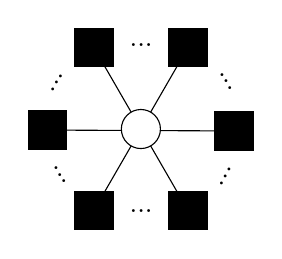
\begin{tikzpicture}[x=0.75pt,y=0.75pt,yscale=-1,xscale=1]
%uncomment if require: \path (0,288); %set diagram left start at 0, and has height of 288

%Shape: Square [id:dp5011100430912303] 
\draw  [fill={rgb, 255:red, 0; green, 0; blue, 0 }  ,fill opacity=1 ] (221.44,121.44) -- (240,121.44) -- (240,140) -- (221.44,140) -- cycle ;
%Shape: Square [id:dp1834276888413744] 
\draw  [fill={rgb, 255:red, 0; green, 0; blue, 0 }  ,fill opacity=1 ] (199.12,159.78) -- (217.68,159.78) -- (217.68,178.34) -- (199.12,178.34) -- cycle ;
%Shape: Square [id:dp4346063530366504] 
\draw  [fill={rgb, 255:red, 0; green, 0; blue, 0 }  ,fill opacity=1 ] (199.12,81.22) -- (217.68,81.22) -- (217.68,99.78) -- (199.12,99.78) -- cycle ;
%Straight Lines [id:da04926983509243965] 
\draw    (230.72,130.72) -- (140.72,130.28) ;
%Straight Lines [id:da6042872004378272] 
\draw    (208.4,169.06) -- (163.04,90.5) ;
%Straight Lines [id:da23454228445560488] 
\draw    (163.04,169.06) -- (208.4,90.5) ;
%Shape: Circle [id:dp7060474924289566] 
\draw  [fill={rgb, 255:red, 255; green, 255; blue, 255 }  ,fill opacity=1 ] (176.31,129.78) .. controls (176.31,124.59) and (180.53,120.37) .. (185.72,120.37) .. controls (190.91,120.37) and (195.13,124.59) .. (195.13,129.78) .. controls (195.13,134.97) and (190.91,139.19) .. (185.72,139.19) .. controls (180.53,139.19) and (176.31,134.97) .. (176.31,129.78) -- cycle ;
%Shape: Square [id:dp12209236616988428] 
\draw  [fill={rgb, 255:red, 0; green, 0; blue, 0 }  ,fill opacity=1 ] (131.44,121) -- (150,121) -- (150,139.56) -- (131.44,139.56) -- cycle ;
%Shape: Square [id:dp4564996494162272] 
\draw  [fill={rgb, 255:red, 0; green, 0; blue, 0 }  ,fill opacity=1 ] (153.76,159.78) -- (172.32,159.78) -- (172.32,178.34) -- (153.76,178.34) -- cycle ;
%Shape: Square [id:dp4857190958072921] 
\draw  [fill={rgb, 255:red, 0; green, 0; blue, 0 }  ,fill opacity=1 ] (153.76,81.22) -- (172.32,81.22) -- (172.32,99.78) -- (153.76,99.78) -- cycle ;

% Text Node
\draw (225,100) node [anchor=north west][inner sep=0.75pt]  [rotate=-60] [align=left] {...};
% Text Node
\draw (221.25,157.5) node [anchor=north west][inner sep=0.75pt]  [rotate=60] [align=left] {...};
% Text Node
\draw (179,87.5) node [anchor=north west][inner sep=0.75pt]   [align=left] {...};
% Text Node
\draw (145,145) node [anchor=north west][inner sep=0.75pt]  [rotate=-60] [align=left] {...};
% Text Node
\draw (179,167.5) node [anchor=north west][inner sep=0.75pt]   [align=left] {...};
% Text Node
\draw (140,112.5) node [anchor=north west][inner sep=0.75pt]  [rotate=60] [align=left] {...};


\end{tikzpicture}

	\caption[Single Variable in a Factor Graph]{A single variable connected to a number of factors}
\end{figure}

One problem still remains with the above setup - a single variable can be connected to any number of factors. As a further simplification, we can group the factors together based off their shared characteristics, which include their origin (if they are internal to the robot or not), their type (what kind of sensor they represent) and their intentions (whether they will help or hinder the robot). For our purposes, we will split the set of factors $F$, into sets $G$ and $B$ based off whether the factors are ``good'' or ``bad'' for the robot. Good factors aim to steer the variable towards the a ground truth value, while bad factors aim to steer it away. Notice that the sets $G$ and $B$ form a cover of $F$, that is $F = G \cup B$.

We then take this a step further and replace each set of factors with a single ``representative factor''.
\begin{figure}[!ht]
	\centering
	

\tikzset{every picture/.style={line width=0.75pt}} %set default line width to 0.75pt        

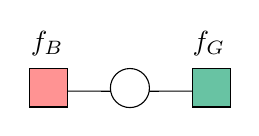
\begin{tikzpicture}[x=0.75pt,y=0.75pt,yscale=-1,xscale=1]
%uncomment if require: \path (0,171); %set diagram left start at 0, and has height of 171

%Straight Lines [id:da9426074160582016] 
\draw    (399.22,143.78) -- (359.94,143.66) ;
%Straight Lines [id:da643000004312603] 
\draw    (399.22,143.78) -- (438.5,143.66) ;
%Shape: Circle [id:dp3724334158586291] 
\draw  [fill={rgb, 255:red, 255; green, 255; blue, 255 }  ,fill opacity=1 ] (389.81,142.22) .. controls (389.81,137.03) and (394.02,132.81) .. (399.22,132.81) .. controls (404.41,132.81) and (408.62,137.03) .. (408.62,142.22) .. controls (408.62,147.41) and (404.41,151.63) .. (399.22,151.63) .. controls (394.02,151.63) and (389.81,147.41) .. (389.81,142.22) -- cycle ;
%Shape: Square [id:dp37804195853429245] 
\draw  [fill={rgb, 255:red, 255; green, 147; blue, 147 }  ,fill opacity=1 ] (350.66,132.81) -- (369.22,132.81) -- (369.22,151.37) -- (350.66,151.37) -- cycle ;
%Shape: Square [id:dp19659269496953535] 
\draw  [fill={rgb, 255:red, 104; green, 195; blue, 163 }  ,fill opacity=1 ] (429.22,132.81) -- (447.78,132.81) -- (447.78,151.37) -- (429.22,151.37) -- cycle ;

% Text Node
\draw (428.22,113.4) node [anchor=north west][inner sep=0.75pt]    {$f_{G}$};
% Text Node
\draw (350.22,113.4) node [anchor=north west][inner sep=0.75pt]    {$f_{B}$};


\end{tikzpicture}


	\caption[Representative factor graph around a single variable]{The above factor graph using ``representative factors''. $f_G$ and $f_B$ respectively represent the sets of good factors ($G$) and bad factors ($B$).}
\end{figure}

We calculate the messages from each of these representative factors as such:
\begin{eqnarray}
	m_{f_G \rightarrow x_i} = \underset{g \in G}{\prod} m_{f_g \rightarrow x_i}&
	m_{f_B \rightarrow x_i} = \underset{b \in B}{\prod} m_{f_b \rightarrow x_i}
\end{eqnarray}
Thus the belief of the variable becomes $p(x) = m_{f_G \rightarrow x} m_{f_B \rightarrow x}$, and since $G \cup B$ covers every factor connected to the variable, we can show that this replacement can be made without altering the variable's final result by equation \ref{eqn:bp_belief}.

\begin{equation}
	p(x_i) = \underset{s \in N(i)}{\prod} m_{f_s \rightarrow x_i}
	\tag{\ref{eqn:bp_belief}}
\end{equation}

For completeness we now present the equations for contents of the messages $m_{f_G \rightarrow x_i}$ and $m_{f_B \rightarrow x_i}$. 
Each message is has an information vector $\eta$ and a precision matrix $\Lambda$.
\begin{eqnarray}
	\eta_G = \underset{g \in G}{\sum} \eta_g&
	\Lambda_G = \underset{g \in G}{\sum} \Lambda_g \label{eqn:good_pull}\\
	\eta_B = \underset{b \in B}{\sum} \eta_b&
	\Lambda_B = \underset{b \in B}{\sum} \Lambda_b \label{eqn:bad_pull}
\end{eqnarray}

\section{Theoretical properties of the RobotWeb under attack}
\subsection{Measuring the strength of an attack}
From the above setup we will now aim to quantify the strength of an attack. For mathematical convenience and ease of understanding, we will derive these equations in 1 dimension, and later present the n-dimensional forms.

To measure the strength of an attack we want to understand the impact of the bad factors on the variable's final belief. To do this we shall use the Kullback-Leibler (KL) divergence \citationneeded between the variable's belief when it is safe and when it is under attack.
The KL divergence is a measure of far the distribution Q is from the distribution P. The further the belief distribution under attack (BDA) is from the distribution suggested by the good factors, the stronger we say the attack is. Similarly, the closer the BDA is to the distribution suggested by the bad factors, the stronger the attack.

The KL divergence between 2 distributions of continuous random variables is:
\begin{equation}
	D_{KL}(P || Q) = \int_{-\infty}^{\infty} log\left( \frac{p(x)}{q(x)} \right) dx
\end{equation}

However a special case exists for Normal distributions, $N_1(\mu_1, \sigma_1^2)$ and $N_2(\mu_2, \sigma_2^2)$.
\begin{equation}
	D_{KL}(N_1 || N_2) = log\left(\frac{\sigma_2}{\sigma_1}\right) + \frac{\sigma_1^2 + (\mu_1 - \mu_2)^2}{2\sigma_2^2} - \frac{1}{2}
\end{equation}

In 1 dimension the messages sent from $f_G$ and $f_B$ are:
\begin{eqnarray}
	m_{f_G \rightarrow x_i} = (\eta_G, \Lambda_G) = (\frac{\mg}{\sgsq}, \frac{1}{\sgsq})\\
	m_{f_B \rightarrow x_i} = (\eta_B, \Lambda_B) = (\frac{\mb}{\sbsq}, \frac{1}{\sbsq}) \label{eqn:attacker_msg}
\end{eqnarray}

From \ref{eqn:bp_belief} we see that the BDA is equal to:
\begin{align}
	m_{f_G \rightarrow x} m_{f_B \rightarrow x} 
	&= (\eta_G + \eta_B, \Lambda_G + \Lambda_B)\\
	&= \left(\frac{\mg}{\sgsq} + \frac{\mb}{\sbsq}, \frac{1}{\sgsq} + \frac{1}{\sbsq}\right)\\
	&= \left(\frac{\mg\sbsq + \mb\sgsq}{\sgsq \sbsq}, \frac{\sbsq + \sgsq}{\sgsq \sbsq}\right)
\end{align}

The above distributions follow the following Normal distributions:
\begin{align}
	G &\sim N\left(\frac{\eta_G}{\Lambda_G}, \frac{1}{\Lambda_G}\right)\\
	B &\sim N\left(\frac{\eta_B}{\Lambda_B}, \frac{1}{\Lambda_B}\right)\\
	BDA &\sim N\left(\mu_{BDA}, \sigma_{BDA}^2\right)\\
	&\sim N\left(\frac{\eta_G + \eta_B}{\Lambda_G + \Lambda_B}, \frac{1}{\Lambda_G + \Lambda_B}\right)\\
	&\sim N\left(\frac{\mg\sbsq + \mb\sgsq}{\sgsq + \sbsq}, \frac{\sgsq \sbsq}{\sgsq + \sbsq}\right) \label{eqn:bda_distribution}
\end{align}

So now we take the KL divergence between the good factors' distribution $G$ and BDA. To make this easier to follow we derive each term in the sum separately.

First deriving the log term we get:
\begin{align}
	log\left(\frac{\sigma_{BDA}}{\sigma_{G}}\right)
	&= log\left(\sqrt[2]{\frac{\sigma_{BDA}^2}{\sigma_{G}^2}}\right)\\
	&= \frac{1}{2} log\left(\frac{\sigma_{BDA}^2}{\sigma_{G}^2}\right)\\
	&= \frac{1}{2} log\left(\frac{\sgsq \sbsq}{\sbsq + \sgsq} \times \frac{1}{\sgsq}\right)\\
	&= \frac{1}{2} log\left(\frac{\sbsq}{\sbsq + \sgsq}\right)
\end{align}

Next we derive the fractional term:
\begin{align}
	\frac{\sigma_{G}^2 + (\mu_{G} - \mu_{BDA})^2}{2\sigma_{BDA}^2}
	&= \frac{
			\sgsq + \left(\mg - \frac{\mg\sbsq + \mb\sgsq}{\sbsq + \sgsq}\right)^2
		}{
			2 \frac{\sgsq \sbsq}{\sbsq + \sgsq}
		}\\
	&= \left(\sgsq + \left(\frac{\mg\sgsq + \mg\sbsq - \mg\sbsq - \mb\sgsq}{\sbsq + \sgsq}\right)^2\right) \times \frac{\sbsq + \sgsq}{2\sgsq\sbsq}\\
	&= \left(\sgsq + \left(\frac{\mg\sgsq - \mb\sgsq}{\sbsq + \sgsq}\right)^2\right) \times \frac{\sbsq + \sgsq}{2\sgsq\sbsq}\\
	&= \frac{\sgsq\left(\sgsq + \sbsq\right)^2 + \left(\mg\sgsq - \mb\sgsq\right)^2}{(\sbsq + \sgsq)^2} \times \frac{\sbsq + \sgsq}{2\sgsq\sbsq}\\
	&= \frac{\sgsq\left(\sgsq + \sbsq\right)^2 + \sigma_G^4\left(\mg - \mb\right)^2}{(\sbsq + \sgsq)^2} \times \frac{\sbsq + \sgsq}{2\sgsq\sbsq}\\
	&= \frac{\left(\sgsq + \sbsq\right)^2 + \sgsq\left(\mg - \mb\right)^2}{2\sbsq(\sbsq + \sgsq)}
\end{align}

Thus the KL divergence between $G$ and BDA is:
\begin{equation}
	\frac{1}{2} log\left(\frac{\sbsq}{\sbsq + \sgsq}\right) + \frac{\left(\sgsq + \sbsq\right)^2 + \sgsq\left(\mg - \mb\right)^2}{2\sbsq(\sbsq + \sgsq)} - \frac{1}{2}
\end{equation}

Similarly the KL divergence between $B$ and BDA is:
\begin{equation}
	\frac{1}{2} log\left(\frac{\sgsq}{\sbsq + \sgsq}\right) + \frac{\left(\sgsq + \sbsq\right)^2 + \sbsq\left(\mg - \mb\right)^2}{2\sgsq(\sbsq + \sgsq)} - \frac{1}{2}
\end{equation}

From this we notice a disturbing detail - the KL divergence is quadratically affected by the $\mb$. This suggests that the attacker's power is unbounded, so long as it chooses an appropriate $\sbsq$. That an attacker can always command a robot to reject the evidence of its own peers and sensors. That the attacker can always craft messages to trick a robot into believing absurdities about its location.

\subsection{Crafting the perfect message}
From the results derived in the previous section, we know that theoretically an attacker will seek to increase its $\mb$ to $\infty$ and decrease its $\sbsq$ to 0. However, in a real life scenario, it is unlikely that the attacker would fully exploit these powers, for two reasons.
\begin{enumerate}
	\item Robots are unlikely to believe \textit{incredibly} incorrect values - no sensible robot would believe that it has moved 500km away in the past 3 seconds.
	\item Robots don't have infinite numerical precision, so large values of $\Lambda_B$ ($\frac{1}{\sbsq}$) would cause overflow errors, which would prevent the attacker from controlling the robot's belief.
\end{enumerate}

Given these restrictions, attackers would set their values of $\mb$ to believable values, whilst choosing the largest value of $\sbsq$ possible. 
We will now suppose that the attacker wishes to move its victim's belief from $\mg$ to $\mt$. \todo{Does the standard deviation matter here?}
As before, the attacker sends a message with the form described in equation \ref{eqn:attacker_msg}.

So from equation \ref{eqn:bda_distribution}, we see that:
\begin{equation}
	\mt = \frac{\mg\sbsq + \mb\sgsq}{\sgsq + \sbsq}
\end{equation}

Which can be rearranged to the form:
\begin{equation}
	\mb = \frac{\mt\left(\sgsq + \sbsq\right) - \mg\sbsq}{\sgsq}
\end{equation}

Which can be used to calculate the $\mb$ that an attacker would send given a minimum $\sbsq$. 
Thus the attacker would send the following message:
\begin{equation}
	\left(\frac{\mt\left(\sgsq + \sbsq\right) - \mg\sbsq}{\sgsq\sbsq}, \frac{1}{\sbsq}\right)
\end{equation}

\subsection{Scaling back up to n-dimensional space}
\todo{TODO: Derive this}

\section{Hypotheses}
In this section, we will present 5 hypotheses about the behaviour of the entire RobotWeb under attack, using the above analysis. These hypotheses will then be experimentally tested in the next section.

\subsection{Bounds on $\mu$ can be slowly escaped} \label{hyp:1}
An intuitive defence against the attackers is setting an upper bound on how far a message can suggest the robot is from its current position belief. 
However, we believe that this approach is ineffective, and can be easily evaded by attackers. In this subsection, we will lay out how this defence would work and how it can be bypassed.

For the upper bound to be effective, it must occupy a ``Goldilocks zone'' - it cannot be too large or too small. If the upper bound is too large, it would present attackers with ample opportunities to control the robot's belief, especially since they aim to suggest somewhat plausible positions.
If the upper bound is too small, it would effectively prevent the robot from listening to any dissenting messages from other good robots.

Now suppose that at time $t$, the robot is at position $\mu_t$ and has a upper bound of $\epsilon$. It would then evaluate each incoming message and reject it if its proposed position $\mu'_t$ is a distance $\epsilon$ away from $\mu_t$. After filtering out all ``bad'' messages, the robot would use the remaining messages to determine $\mu_{t+1}$. 

Being aware of this scheme, and attacker would seek to incrementally attack the robot. It would start by proposing a position $\mu''_t$ that lies between $\mu_t$ and its target location $\mu'_t$, such that $\mu''_t$ is accepted by the robot. This would successfully shift the robot's position estimate $\mu_{t+1}$ to $\mu''_t$. In the next iteration, the robot would reject any proposals a distance of $\epsilon$ away from $\mu_{t+1} = \mu''_t$. Hence over several iterations, the robot's position estimate would slowly shift to $\mu'_t$, and thus the attacker would be able to escape the bound.
\todo{Would a diagram be useful here?}

\subsection{Bounds on $\Lambda$ can be quickly escaped} \label{hyp:2}
As shown previously, the strength of an attack is highly dependent on its ability to propose arbitrary values of $\Lambda$. Which leads to another intuitive defence strategy - robots set an upper bound on the $\Lambda$ values that they receive. We believe that this strategy is effective when there is only a single identity spreading misinformation, counterbalanced by many others sending reliable information. In this subsection, we will provide a justification for this belief as well as a strategy that an attacker could take to bypass the upper bound on $\Lambda$.

The $\Lambda$ value of a message can be though of as its ``pull'', or how strongly the message would move a variable towards its proposed location. The greater the value, the stronger the pull. \todo{Norms?} With this in mind, we can think of the robot's location estimate as being ``pulled'' by good and bad factors, where good factors pull the estimate towards a ground truth, whilst bad factors pull it to an alternate location. 

When sending a message, each robot decides the strength of the message's pull. Good robots limit their strength to the accuracy of their sensors, while attackers will set their strength to the fullest extent. This once again makes the case for the use of a reasonable upper bound on the strength of a message, similar to the one described above.

We argue that this upper bound is unenforceable in practice, for an attacker can simply ``split'' their message into several weaker parts. So far in our analysis, we have treated $\Lambda_B$ as if it were sent in a single message, however from equation \ref{eqn:bad_pull} we can see that it may also be the result of several bad robots sending messages. In fact, if the upper bound on an individual message's $\Lambda$ is $\lambda$, then an attacker could simply send several messages from several different identities to arrive at a strong $\Lambda_B$, in a Sybil Attack. \todo{Should I add maths here too?}
\subsubsection{Aside: Attacks are uncorrelated} \label{hyp:2.5}
Considering the ``pull based model'' of variables, it stands to reason that in a Sybil Attack, the messages sent by individual identities will not be correlated with each other, as that would greatly simplify the detection and prevention of attacks. Instead, we believe that Sybil Attackers would send messages with wildly different $\mu$ values, that would ``resolve'' to the actual attack that the attacker intends.

\subsection{Long histories are detrimental} \label{hyp:3} % History can be weaponised
One little discussed feature of the RobotWeb so far has been its time-windowed history. Instead of remembering every past position that that robot has had, it instead chooses to only remember the past $h$ positions. This improves the performance of robots in the RobotWeb, as they store fewer pose variables and thus perform fewer floating-point operations when updating beliefs. In the original paper, Murai et al. show that the impact of time-windowed history on the average trajectory error of each robot is negligible.

\todo{Add graph}

We believe that keeping the full position history not only has an adverse impact on the compuational performance of a robot, but also amplifies the strength of attacks. If an attacker is able to successfully attack a robot at time $t$, then the pose variable at $t$, $v_t$ will contain a $\mu$ close to the attacker's target $\mu$, and its $\Lambda$ will be high. If $v_t$ is then used to estimate the robot's position at time $t+1$, then it will effectively also attack the robot, as it would further the attacker's belief. The longer the history kept by a robot, the more power an attacker can gain over it.

\subsection{Attacks can spread on their own} \label{hyp:4} % A falling tide sinks all ships/Can't let the genie out of the bottle
Similarly to the previous hypothesis, we can assume that any other variable connected to $v_t$ will be attacked by it. Thus a victim of an attack will unintentionally attack all those it contacts, meaning that attacks have a degree of contagion. 

Attackers may not be able to prevent or limit contagion, as they would need to strongly pull unintentional victims back to a ground truth value. Since no robot has absolute certainty about the locations of any other, the attacker will actually pull them to values close to their ground truth. However, as there is no mechanism to increase $\Lambda$, the attacker will still make the other robots overconfident about their locations, which may bias them in the long term.
\subsection{Robots are most vulnerable on startup} \label{hyp:5}
Our final hypothesis is that robots that have just started up are likely to be the most affected by attacks, as they wouldn't have a strong estimate of their location. This would mean that their $\Lambda_G$ is much lower than older robots, increasing the strength of the attack.

\section{Experimental evidence}

Now, we will evaluate the above hypotheses in a simulated environment. Our goal is to show that the predicted phenomena can arise, rather than guaranteeing their emergence. The reasoning behind this is that an attack only needs to be successful in a single situation for it to be considered potent.

\subsection{Experimental setup}
We will use an adapted version of the simulator detailed in \cite[RobotWeb]{Robotweb} for our experiments. Each simulation will contain a single attacking robot and $n$ normal robots. Each robot will move along a predefined path, and aim to localise well to that path - this will be challenged by the attacker, which will attempt to trick them into localising to a path of its choosing.

Furthermore each robot in the simulation will carry 2 sensors; one for odometry and one for measuring others. The odometry sensor will be used by a robot to estimate its current location using its previous location and its motion. The range-bearing sensor will be used to measure other robots - it will measure the distance between the 2 robots and the bearing of the other robot from this one. All robots' range-bearing sensors have a range limit; however, attackers will ignore this as they always know where they want their victims to be.

The simulation has several configurable parameters which we will vary in our experiments. We detail the most important ones below.

% TODO: make table good
% QUESTION: Should I explain how likely robots are to measure each other?
\renewcommand{\arraystretch}{1.35}
\begin{table}[ht]
\centering
\begin{tabular}{|c|c|c|}
\hline
\textbf{Parameter}    & \textbf{Description}                                                                                                          & \textbf{Default values}                                                                                        \\ \hline
Dataset               & The physical path travelled by each robot.                                                                                    & See below                                                                                                      \\ \hline
Attacker Dataset      & \begin{tabular}[c]{@{}c@{}}The path attackers attempt to trick the robot \\ into localising onto\end{tabular}                 & See below                                                                                                      \\ \hline
Sliding Window Bucket & \begin{tabular}[c]{@{}c@{}}The number of historical pose variables \\ used by each robot (aka the history size).\end{tabular} & 2                                                                                                             \\ \hline
N iterations per step & \begin{tabular}[c]{@{}c@{}}The number of GBP iterations performed\\  every time the robot moves.\end{tabular}                 & 10                                                                                                             \\ \hline
SE2 Prior             & The accuracy of each robot's original position.                                                                               & \begin{tabular}[c]{@{}c@{}}$\sigma_x = 1e^{-8}$ m\\ $\sigma_y = 1e^{-8}$ m\end{tabular}                        \\ \hline
Between SE2           & The accuracy of each robot's odometry sensor.                                                                                 & \begin{tabular}[c]{@{}c@{}}$\sigma_x = 0.1$ m\\  $\sigma_y = 0.1$ m \\ $\sigma_\theta = 0.01$ rad\end{tabular} \\ \hline
Sensor range limit    & The furthest a range-bearing sensor can detect.                                                                               & 0.25 m                                                                                                         \\ \hline
Sensor noise model    & \begin{tabular}[c]{@{}c@{}}The noise associated with the \\ range and bearing measurements.\end{tabular}                      & \begin{tabular}[c]{@{}c@{}}$\sigma_r = 0.05$ m\\ $\sigma_\theta = 0.1$ rad\end{tabular}                        \\ \hline
Attacker confidence   & \begin{tabular}[c]{@{}c@{}}The confidence claimed by the attacker.\end{tabular}                      & \begin{tabular}[c]{@{}c@{}}$\sigma_x = 0.001$ m\\ $\sigma_y = 0.001$ m\end{tabular} \\ \hline
\end{tabular}
\end{table}

\subsubsection{Path design}
Since the RobotWeb currently hasn't been deployed, we are faced with a dearth of real-world paths for our experiments. This leaves us with the choice of either inventing a realistic path or using a simple, artificial path. For the following experiments, we have chosen to use simple paths as we aim to show that these phenomena can arise. Later we will test our defences on more realistic paths.

%TODO: Add image

We choose to use the above paths to test. The robots will move along the green path, whilst the attackers will try to convince them that they are instead moving along the red path. The robots belief of their path is the black path. The attacker takes the bottom path.

%TODO: Sort out the measurement units

\subsection{Testing hypothesis 1}
The first hypothesis, \ref{hyp:1}, predicts that attackers can overcome bounds on $\mu$, by performing incremental attacks. We test this using 2 robots; an attacker and its victim. For the victim, we introduce a $\mu$ bound defence of 0.05m, so that it only believes messages which are within a 0.05m radius from its current position estimate. For the attacker, we add an onramp composed of several segments, to transition the victim to the attacker's desired path. We vary the length of the onramp's segments and measure the victim's Average Trajectory Error (ATE) over 10 runs.

%TODO: Add diagram to show onramp

Analysing the ATE against segment length, we see that a cliff emerges, where once the segments are short enough, the ATE significantly increases, indicating a successful attack. Thus confirming the first hypothesis, that an attacker can overcome bounds on $\mu$.

%TODO: Add graph

Interestingly enough, we also see that the cliff starts a little short of the $\mu$ bound. This effect occurs as the victim's position estimate is noisy, leading it to occasionally accept the attacker's messages. Every time the victim accepts one of these messages, it's pulled closer to the attacker's desired path, which in turn makes it more likely to accept the attacker's future messages.

Looking at the victim's ATE over time in the below graph, we see that the victim's ATE only increases once it is firmly on the onramp. This means that the $\mu$ bound defence still hinders the attacker, as it must both create an onramp and wait for its victim to traverse it.

%TODO: Add graph

\subsection{Testing hypothesis 2}
The second hypothesis, \ref{hyp:2}, asserts that an attacker can carry out an attack without manipulating its confidence level, instead the attacker would send many messages under many fake identities. We test this using 11 robots; an attacker and its 10 victims. We also prevent the attacker from altering the confidence level of any of the messages it sends. We vary the number of false identities that the attacker creates, and measure the average ATE across each victim. We repeat this experiment 10 times.

From the above graph, we can see that as the number of false identities grows, so too does the average ATE. Unlike the previous experiment, when we analyse the ATE over time, we see that the effect of this attack has no delay, making it more potent. These two observations thus confirm the second hypothesis.

\subsection{Testing hypothesis 3}
The third hypothesis suggests that robots keeping longer histories are more vulnerable to attacks. We test this using 2 robots; an attacker and its victim. We vary the victim's history size and measure its ATE. In order to accurately gauge the effect of the history size, we also weaken the attacker's attacks by reducing its confidence such that $\sigma_x = \sigma_y = 10$ m. We repeat this experiment 10 times.

% Figure out how this would work.

Looking at the ATE against history size when an attacker is present reveals that longer histories do in fact harm robots' localisation, but only until a point after which this effect levels off. This is likely due to the fact that the past poses are fully attacked by then, and so can't attack the robots further.

Looking at the ATE against history size when no attackers are present, tells the opposite story - that a longer history does help in the good times, albeit very slightly. We believe that this effect is only due to the fact that the robots have good odometry, which leads us to rerun the experiment with worse odometry sensors. We can now see a more pronounced positive effect of longer history vectors, which again levels off.

This suggests that for real-world scenarios there will always be a trade-off to be considered. Longer histories may improve localisation when no attacks are taking place but at the cost of increased risk and a higher computational load.

\subsection{Testing hypothesis 4}
The fourth hypothesis predicts that attacks will spread without the active involvement of the attacker, where the victims inadvertently will attack other robots. We test this using 11 robots; an attacker, its victim and 9 other robots. We devise a special configuration for this experiment where the attacker only communicates with its victim, and only adjacent robots can communicate with each other. This provides us with a daisy chain communication pattern, where the victim's attack must take several ``hops'' to reach the ends of the chain. We then measure the ATE of each robot over 10 runs. For this experiment, we utilise a control group, in which there is no attacker, to highlight the effect of the attacker.

 % TODO: graph

Looking at the above graph, we can see that the few number of hops from a robot to the victim, the higher its ATE will be. We also see that the ATE of every robot in the attacked group is higher than in the control group, which proves the existence of this contagion effect - thus proving the hypothesis.

This effect prevents real-world attackers from relying on any robots in the vicinity of their victims, lest they are themselves attacked by their own attack. This serves as a small penalty for misbehaviour but is not sufficient to deter a motivated attacker.

\subsection{Testing hypothesis 5}
The fifth and final hypothesis posits that young robots which have recently joined the web will be the most vulnerable to attacks. We test using 2 robots; an attacker and its victim. We introduce a delay between when the victim starts and when it joins the network. We then measure the ATE of the victim across 10 runs. We also vary the victim's history size, as we believe that there is likely a link between the optimum startup delay of a robot and the size of its history.

Looking at the above heatmap, we see that the startup delay does provide a small defence against the attacker, but that its strength diminishes as the delay lengthens. We also see a clear correlation between the effect of the startup delay and the history size used by the victim.

These results suggest that a small startup delay does provide a defence against attacks, although it is inadequate to fully defend the robot. We also see that the startup delay does not significantly hinder localisation in the absence of attackers, meaning that it is a cheap defence that can be used.

% TODO: Add a conclusions section?
\chapter{Defending the RobotWeb}
This chapter serves as a dual to the previous chapter. Here we will use our understanding of the RobotWeb under attack to design and evaluate Aegis, a group-based defence algorithm. First, we will establish the definition of defence in the Robotweb. Subsequently, we will discuss the shortcomings of individualistic defence strategies. Then we shall outline the conceptual backbone of our defence, and evaluate it in realistic scenarios. Finally, we will evaluate some improvements to this defence.

\section{A Definition of Defence}
A robot is well-defended against attackers if it can guarantee that it cannot be forced to localise at an arbitrary point. This means that a well-defended robot's belief of its trajectory will closely follow its actual trajectory. There are two avenues to obtaining this guarantee; the robot could either reject all messages from attackers or secondly, it could reject all messages which move it too far from its ground truth. We consider robots taking the first avenue to be \textbf{strongly-defended} (\autoref{prop:strong-def}) and robots taking the second avenue to be \textbf{weakly-defended} (\autoref{prop:weak-def}).

\begin{prop}[Strong-Defendedness]
\label{prop:strong-def}
A strongly-defended robot, $r_s$, will reject any message $m_i$ if that message was sent by another robot, $r_i$, if $r_i$ is an attacker.
\end{prop}

\begin{prop}[Weak-Defendedness]
\label{prop:weak-def}
A weakly-defended robot located at $\mu_{gt}$ will reject any message $m_i$ if that message would force it to localise further than a distance $\epsilon$ away from $\mu_{gt}$. Put formally: \[\norm{\mu_{gt} - \mu_i} \leq \epsilon\]
\end{prop}

Strong defences are the ideal defences since they allow the RobotWeb to function as if no attackers were present. However, these strategies face the challenge of correctly identifying attackers. A good robot misclassified as an attacker leads to a slight decrease in localisation accuracy, whereas an attacker misclassified as a good robot can be catastrophic. This is further complicated by our findings from the previous chapter, namely subsections \ref{hyp:mu_bound} and \ref{hyp:sybils}, which show that it is very difficult to distinguish between attackers' messages and those of good robots. A simple, if naive strategy that solves this, is for a robot to reject \emph{every} message sent to it - it cannot accept an attacker's message if it doesn't accept any message. Yet this has little benefit, as now the robot no longer benefits from participating in the RobotWeb.

Weak defences, on the other hand, do not guarantee a robot's safety, but they compensate for this by being more resilient to attacks, if and when they happen. If a strong defence scheme accidentally accepts an attacker's message, then it's checkmate, but a weak defence scheme may accept the same attacker's message without experiencing the same disastrous consequences. Yet the implementation of a weak defence is not without its problems. 

Before a weakly-defended robot can reject a message, it must first know its ground truth pose, or have a good approximation of it. Getting this ground truth pose is the main hurdle for weak defence strategies since the RobotWeb primarily operates using relative measurements i.e. where one robot is from the perspective of another, rather than absolute measurements i.e. GPS. The only two sources of ground truth information in the RobotWeb are: \begin{enumerate*}
    \item a robot's initial localisation and
    \item the localisations of beacons
\end{enumerate*}. Neither of which can be relied upon here. A robot's initial localisation becomes less relevant as the robot moves and accumulates noise, whilst beacons may themselves act as attackers.

\section{The Limits of Individualism} \label{section:indiv-limits}
When designing defences for the RobotWeb, one may intuitively reach for individualistic approaches, where a robot can defend itself without relying upon any third party. These approaches have some merit, namely, they ensure that a robot can \textit{always} defend itself. This self-reliance serves as an effective deterrent to attackers, who know that any attack via the RobotWeb will be ineffective, and so won't attack through it. Essentially, if an entirely trustless defence exists, it would allow robots to fully and fearlessly participate in the RobotWeb. In this section, we argue that this is not possible.

For a robot to follow a strong, individualistic defence strategy, it would need to find a method to trust good robots and mistrust attackers. One such approach would be for it to use its internal odometry sensors to verify the veracity of messages. However, as we have previously seen (\ref{hyp:mu_bound}, \ref{hyp:sybils}, \ref{hyp:uncorrelated_sybils}), such measures can be easily circumvented. Another set of approaches involves robots signalling their credibility to their peers, such that robots spreading misinformation are heavily penalised.

One such approach would be to use a reputation system, where messages from robots with a higher reputation are given a higher weight than those with lower reputations. A robot's reputation would increase with every correct message it sends, and decrease with every incorrect message. Robots would decide the correctness of a message by measuring how well it aligns with their current beliefs - the better the alignment the more likely the message is to be correct. Reputation systems come in 2 distinct flavours, local and global. 

In a global reputation system, all robots in the RobotWeb would collectively track one anothers' reputations, so discovered attackers would be universally distrusted. However, attackers could also attempt to lower the reputations of good robots by claiming that \textit{they} themselves are victims of the good robots. This presents a problem, as now robots need a mechanism to verify misinformation claims, yet if such a mechanism existed then they would not need to rely on a global information system. This leads us to conclude that a global reputation system is not a viable solution here.

Alternatively, in a local reputation system, each robot maintains its own set of beliefs about the reputations of those it encounters. This eliminates the need for multiple robots to reconcile their reputation beliefs and thus prevents attackers from attacking the reputations of others. However, this still falls prey to problems that haunt all reputation systems. Firstly, an attacker can reset its reputation by simply changing its identity. Secondly, an attacker can amass a significant amount of reputation through the use of Sybils, which it would then use to attack.

Another approach would be to use computational resources to provide credible signals akin to Proof of Work systems. The philosophy behind this approach is that misinformation would be too costly to spread, and thus no attacks would take place. However, as we have shown in the background section, schemes using computational resources fall flat due to the heterogeneity of the RobotWeb - some robots may run on microcontrollers whilst others feature GPUs, which would mean that larger robots could easily spread misinformation to smaller ones.

A similar approach, Proof of Stake \cite{pos}, does not fare much better. Proof of Stake replaces the computational resources in Proof of Work, with financial resources. If Proof of Stake were to be used here, then robots would post collateral with every message they sent, such that they would lose this collateral if they were found to be spreading misinformation. However, this approach is also infeasible as it is still impossible for a robot to prove that antoher is misinforming it.

To conclude, we believe that individualistic approaches to defence are generally infeasible. Firstly, they lack a method for reliably estimating a ground truth pose and so cannot filter out messages by content. Secondly, it is likely that any motivated attack will treat all penalties as prices, so these approaches cannot deter sufficiently motivated attackers It is for these reasons that we turn to systems with a degree of partial for our solution.

\section{The Aegis Defence} \label{section:aegis}
Given that individualistic approaches to defence fail to protect robots against attacks, we now present Aegis, a group-based defence algorithm. Here robots will organise themselves into local groups, where each robot implicitly trusts the others in its group. Importantly, the mechanism that allows for this trust is external to the RobotWeb, meaning that the amount of trust one robot has in another no longer depends on how it behaves, but is instead fixed by its operator. 

As an example, we consider a situation where Alice operates several robots, and a hostile Charlie operates an attacker. Alice may provide each of her robots with a list of other robots that they can trust, i.e. each other. Now Alice's robots will only trust others that can prove that they're included in the list. This proof can be securely generated using existing cryptographic techniques, for example in \cite{zkp}. This ensures that despite its best efforts, Charlie's attacker cannot trick Alice's robots into trusting it.

Using this mutual trust mechanism, robots in a group will automatically assign themselves one of 2 roles; strongly-defended \textbf{leaders} and weakly-defended \textbf{followers}. The leaders of a group are responsible for protecting both themselves and their followers. A leader will protect itself by rejecting all messages from robots that aren't its fellow leaders. The leader will then protect its followers by providing them with an approximation of their ground truth poses, which they will use to weakly defend themselves from attack. Meanwhile, followers have no such responsibilities neither toward leaders nor towards any other robot.

It is important to note that the concept of a group is a local one and there is no shared global group. Instead, groups will constantly be formed and dissolved, using the mutual trust mechanism. If a robot observes several others that it can trust, it will consider them a part of its group. If it then encounters another that it can trust, then it will absorb it into its group. If a robot stops observing some group members, then it will stop considering them as part of its group. Essentially, a robot will only consider those it can observe as part of its group. We made this design decision to reflect upon the spatial nature of multi-robot systems, where only observable robots are relevant to one another. Note that a robot can observe others without necessarily sensing them, instead they must merely be within its communication range. 

\begin{figure}[!h]
	\centering
	

\tikzset{every picture/.style={line width=0.75pt}} %set default line width to 0.75pt        

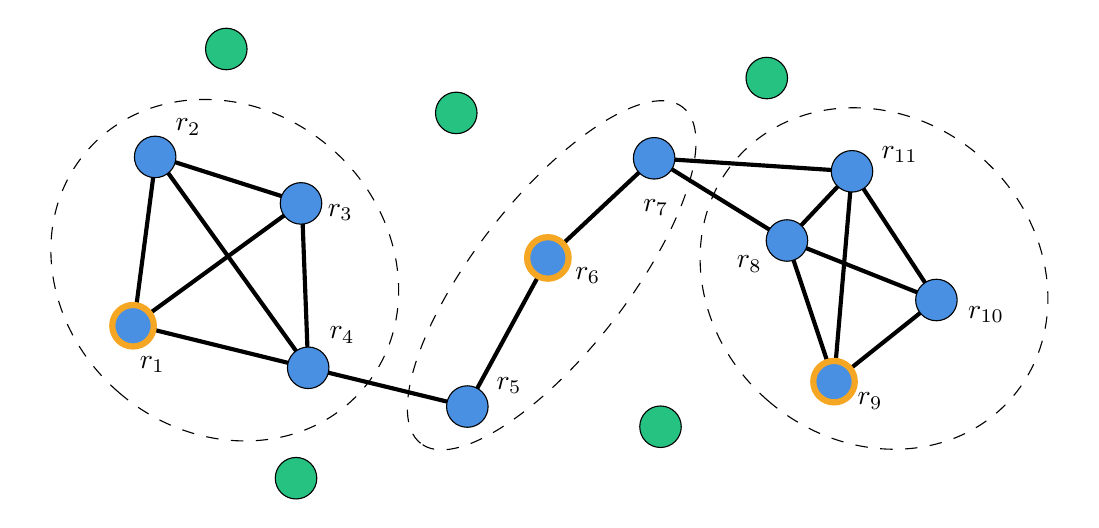
\begin{tikzpicture}[x=0.75pt,y=0.75pt,yscale=-1,xscale=1]
%uncomment if require: \path (0,300); %set diagram left start at 0, and has height of 300

%Straight Lines [id:da821267233332613] 
\draw [line width=1.5]    (122,74.33) -- (111.33,155.67) ;
%Straight Lines [id:da30341458803905486] 
\draw [line width=1.5]    (192.27,96.73) -- (122,74.33) ;
%Straight Lines [id:da15308567646882731] 
\draw [line width=1.5]    (192.27,96.73) -- (111.33,155.67) ;
%Straight Lines [id:da8895692654604979] 
\draw [line width=1.5]    (195.33,176.33) -- (111.33,155.67) ;
%Straight Lines [id:da8452110592323836] 
\draw [line width=1.5]    (195.33,176.33) -- (122,74.33) ;
%Straight Lines [id:da0975036779101448] 
\draw [line width=1.5]    (195.33,176.33) -- (192.27,96.73) ;
%Straight Lines [id:da6708709230251428] 
\draw [line width=1.5]    (426,115) -- (457.33,81.67) ;
%Straight Lines [id:da888005791791295] 
\draw [line width=1.5]    (448.67,183) -- (498,143.67) ;
%Straight Lines [id:da336628623261488] 
\draw [line width=1.5]    (448.67,183) -- (426,115) ;
%Straight Lines [id:da4856371467801972] 
\draw [line width=1.5]    (498,143.67) -- (457.33,81.67) ;
%Straight Lines [id:da9180518393029332] 
\draw [line width=1.5]    (498,143.67) -- (426,115) ;
%Straight Lines [id:da8952427329272475] 
\draw [line width=1.5]    (448.67,183) -- (457.33,81.67) ;
%Straight Lines [id:da8036283886157122] 
\draw [line width=1.5]    (272,195) -- (195.33,176.33) ;
%Straight Lines [id:da5584979597450603] 
\draw [line width=1.5]    (272,195) -- (311.2,123) ;
%Straight Lines [id:da816703332184367] 
\draw [line width=1.5]    (311.2,123) -- (362,75.4) ;
%Straight Lines [id:da907029535911398] 
\draw [line width=1.5]    (362,75.4) -- (457.33,81.67) ;
%Straight Lines [id:da5919582697274625] 
\draw [line width=1.5]    (362,75.4) -- (426,115) ;
%Shape: Circle [id:dp347326930362014] 
\draw  [fill={rgb, 255:red, 74; green, 144; blue, 226 }  ,fill opacity=1 ] (111.6,74.73) .. controls (111.6,69.21) and (116.08,64.73) .. (121.6,64.73) .. controls (127.12,64.73) and (131.6,69.21) .. (131.6,74.73) .. controls (131.6,80.26) and (127.12,84.73) .. (121.6,84.73) .. controls (116.08,84.73) and (111.6,80.26) .. (111.6,74.73) -- cycle ;
%Shape: Circle [id:dp9802636371346682] 
\draw  [fill={rgb, 255:red, 74; green, 144; blue, 226 }  ,fill opacity=1 ] (185.33,176.33) .. controls (185.33,170.81) and (189.81,166.33) .. (195.33,166.33) .. controls (200.86,166.33) and (205.33,170.81) .. (205.33,176.33) .. controls (205.33,181.86) and (200.86,186.33) .. (195.33,186.33) .. controls (189.81,186.33) and (185.33,181.86) .. (185.33,176.33) -- cycle ;
%Shape: Circle [id:dp48904188057709364] 
\draw  [color={rgb, 255:red, 245; green, 166; blue, 35 }  ,draw opacity=1 ][fill={rgb, 255:red, 74; green, 144; blue, 226 }  ,fill opacity=1 ][line width=2.25]  (100.93,156.07) .. controls (100.93,150.54) and (105.41,146.07) .. (110.93,146.07) .. controls (116.46,146.07) and (120.93,150.54) .. (120.93,156.07) .. controls (120.93,161.59) and (116.46,166.07) .. (110.93,166.07) .. controls (105.41,166.07) and (100.93,161.59) .. (100.93,156.07) -- cycle ;
%Shape: Circle [id:dp973523892724249] 
\draw  [fill={rgb, 255:red, 74; green, 144; blue, 226 }  ,fill opacity=1 ] (181.87,97.13) .. controls (181.87,91.61) and (186.34,87.13) .. (191.87,87.13) .. controls (197.39,87.13) and (201.87,91.61) .. (201.87,97.13) .. controls (201.87,102.66) and (197.39,107.13) .. (191.87,107.13) .. controls (186.34,107.13) and (181.87,102.66) .. (181.87,97.13) -- cycle ;
%Shape: Circle [id:dp5060420763706514] 
\draw  [fill={rgb, 255:red, 74; green, 144; blue, 226 }  ,fill opacity=1 ] (447.33,81.67) .. controls (447.33,76.14) and (451.81,71.67) .. (457.33,71.67) .. controls (462.86,71.67) and (467.33,76.14) .. (467.33,81.67) .. controls (467.33,87.19) and (462.86,91.67) .. (457.33,91.67) .. controls (451.81,91.67) and (447.33,87.19) .. (447.33,81.67) -- cycle ;
%Shape: Circle [id:dp8643742073771314] 
\draw  [fill={rgb, 255:red, 74; green, 144; blue, 226 }  ,fill opacity=1 ] (488,143.67) .. controls (488,138.14) and (492.48,133.67) .. (498,133.67) .. controls (503.52,133.67) and (508,138.14) .. (508,143.67) .. controls (508,149.19) and (503.52,153.67) .. (498,153.67) .. controls (492.48,153.67) and (488,149.19) .. (488,143.67) -- cycle ;
%Shape: Circle [id:dp32518754630200464] 
\draw  [fill={rgb, 255:red, 74; green, 144; blue, 226 }  ,fill opacity=1 ] (416,115) .. controls (416,109.48) and (420.48,105) .. (426,105) .. controls (431.52,105) and (436,109.48) .. (436,115) .. controls (436,120.52) and (431.52,125) .. (426,125) .. controls (420.48,125) and (416,120.52) .. (416,115) -- cycle ;
%Shape: Circle [id:dp1004066872083681] 
\draw  [color={rgb, 255:red, 245; green, 166; blue, 35 }  ,draw opacity=1 ][fill={rgb, 255:red, 74; green, 144; blue, 226 }  ,fill opacity=1 ][line width=2.25]  (438.67,183) .. controls (438.67,177.48) and (443.14,173) .. (448.67,173) .. controls (454.19,173) and (458.67,177.48) .. (458.67,183) .. controls (458.67,188.52) and (454.19,193) .. (448.67,193) .. controls (443.14,193) and (438.67,188.52) .. (438.67,183) -- cycle ;
%Shape: Circle [id:dp13679157078018644] 
\draw  [fill={rgb, 255:red, 74; green, 144; blue, 226 }  ,fill opacity=1 ] (262,195) .. controls (262,189.48) and (266.48,185) .. (272,185) .. controls (277.52,185) and (282,189.48) .. (282,195) .. controls (282,200.52) and (277.52,205) .. (272,205) .. controls (266.48,205) and (262,200.52) .. (262,195) -- cycle ;
%Shape: Circle [id:dp6424299525506494] 
\draw  [color={rgb, 255:red, 245; green, 166; blue, 35 }  ,draw opacity=1 ][fill={rgb, 255:red, 74; green, 144; blue, 226 }  ,fill opacity=1 ][line width=2.25]  (300.8,123.4) .. controls (300.8,117.88) and (305.28,113.4) .. (310.8,113.4) .. controls (316.32,113.4) and (320.8,117.88) .. (320.8,123.4) .. controls (320.8,128.92) and (316.32,133.4) .. (310.8,133.4) .. controls (305.28,133.4) and (300.8,128.92) .. (300.8,123.4) -- cycle ;

%Shape: Circle [id:dp3408789117010794] 
\draw  [fill={rgb, 255:red, 74; green, 144; blue, 226 }  ,fill opacity=1 ] (352,75.4) .. controls (352,69.88) and (356.48,65.4) .. (362,65.4) .. controls (367.52,65.4) and (372,69.88) .. (372,75.4) .. controls (372,80.92) and (367.52,85.4) .. (362,85.4) .. controls (356.48,85.4) and (352,80.92) .. (352,75.4) -- cycle ;
%Shape: Ellipse [id:dp9780793680593792] 
\draw  [dash pattern={on 4.5pt off 4.5pt}] (249.5,212.72) .. controls (233.44,200.19) and (248.69,153.79) .. (283.56,109.07) .. controls (318.43,64.36) and (359.72,38.26) .. (375.78,50.79) .. controls (391.84,63.31) and (376.59,109.72) .. (341.72,154.43) .. controls (306.85,199.15) and (265.56,225.24) .. (249.5,212.72) -- cycle ;
%Shape: Ellipse [id:dp17464640664522002] 
\draw  [dash pattern={on 4.5pt off 4.5pt}] (104.43,188.51) .. controls (67.6,156.96) and (60.44,104.88) .. (88.44,72.19) .. controls (116.44,39.5) and (169,38.57) .. (205.84,70.11) .. controls (242.67,101.66) and (249.83,153.74) .. (221.83,186.43) .. controls (193.82,219.13) and (141.26,220.06) .. (104.43,188.51) -- cycle ;
%Shape: Ellipse [id:dp7547054439217645] 
\draw  [dash pattern={on 4.5pt off 4.5pt}] (417.23,192.51) .. controls (380.4,160.96) and (373.24,108.88) .. (401.24,76.19) .. controls (429.24,43.5) and (481.8,42.57) .. (518.64,74.11) .. controls (555.47,105.66) and (562.63,157.74) .. (534.63,190.43) .. controls (506.62,223.13) and (454.06,224.06) .. (417.23,192.51) -- cycle ;
%Shape: Circle [id:dp07179305757060428] 
\draw  [fill={rgb, 255:red, 38; green, 194; blue, 129 }  ,fill opacity=1 ] (256.67,53.53) .. controls (256.67,48.01) and (261.14,43.53) .. (266.67,43.53) .. controls (272.19,43.53) and (276.67,48.01) .. (276.67,53.53) .. controls (276.67,59.06) and (272.19,63.53) .. (266.67,63.53) .. controls (261.14,63.53) and (256.67,59.06) .. (256.67,53.53) -- cycle ;
%Shape: Circle [id:dp6276221659819717] 
\draw  [fill={rgb, 255:red, 38; green, 194; blue, 129 }  ,fill opacity=1 ] (355.07,204.73) .. controls (355.07,199.21) and (359.54,194.73) .. (365.07,194.73) .. controls (370.59,194.73) and (375.07,199.21) .. (375.07,204.73) .. controls (375.07,210.26) and (370.59,214.73) .. (365.07,214.73) .. controls (359.54,214.73) and (355.07,210.26) .. (355.07,204.73) -- cycle ;
%Shape: Circle [id:dp8257521060147176] 
\draw  [fill={rgb, 255:red, 38; green, 194; blue, 129 }  ,fill opacity=1 ] (179.47,229.53) .. controls (179.47,224.01) and (183.94,219.53) .. (189.47,219.53) .. controls (194.99,219.53) and (199.47,224.01) .. (199.47,229.53) .. controls (199.47,235.06) and (194.99,239.53) .. (189.47,239.53) .. controls (183.94,239.53) and (179.47,235.06) .. (179.47,229.53) -- cycle ;
%Shape: Circle [id:dp5988037975306492] 
\draw  [fill={rgb, 255:red, 38; green, 194; blue, 129 }  ,fill opacity=1 ] (145.87,22.73) .. controls (145.87,17.21) and (150.34,12.73) .. (155.87,12.73) .. controls (161.39,12.73) and (165.87,17.21) .. (165.87,22.73) .. controls (165.87,28.26) and (161.39,32.73) .. (155.87,32.73) .. controls (150.34,32.73) and (145.87,28.26) .. (145.87,22.73) -- cycle ;
%Shape: Circle [id:dp013478726522430984] 
\draw  [fill={rgb, 255:red, 38; green, 194; blue, 129 }  ,fill opacity=1 ] (406.27,36.73) .. controls (406.27,31.21) and (410.74,26.73) .. (416.27,26.73) .. controls (421.79,26.73) and (426.27,31.21) .. (426.27,36.73) .. controls (426.27,42.26) and (421.79,46.73) .. (416.27,46.73) .. controls (410.74,46.73) and (406.27,42.26) .. (406.27,36.73) -- cycle ;

% Text Node
\draw (112.93,169.47) node [anchor=north west][inner sep=0.75pt]    {$r_{1}$};
% Text Node
\draw (130.2,55.2) node [anchor=north west][inner sep=0.75pt]    {$r_{2}$};
% Text Node
\draw (203.6,96.4) node [anchor=north west][inner sep=0.75pt]    {$r_{3}$};
% Text Node
\draw (204.4,155.4) node [anchor=north west][inner sep=0.75pt]    {$r_{4}$};
% Text Node
\draw (284.8,179.6) node [anchor=north west][inner sep=0.75pt]    {$r_{5}$};
% Text Node
\draw (322.8,126.8) node [anchor=north west][inner sep=0.75pt]    {$r_{6}$};
% Text Node
\draw (355.6,94) node [anchor=north west][inner sep=0.75pt]    {$r_{7}$};
% Text Node
\draw (400.6,121.2) node [anchor=north west][inner sep=0.75pt]    {$r_{8}$};
% Text Node
\draw (458.8,187.2) node [anchor=north west][inner sep=0.75pt]    {$r_{9}$};
% Text Node
\draw (512,145.6) node [anchor=north west][inner sep=0.75pt]    {$r_{10}$};
% Text Node
\draw (470.4,68.4) node [anchor=north west][inner sep=0.75pt]    {$r_{11}$};


\end{tikzpicture}


	\caption[Dynamic Groups]{An illustration showing the dynamic nature of groups. Here we have blue and green robots, where every blue robot only trusts other blue robots. A line between the pair of robots $r_i$ and $r_j$ indicates that they can observe one another. Robots with a golden outline are leaders, whilst the others are followers. We see that $r_1$ can observe  $r_2$, $r_3$ and $r_4$. Similarly, $r_6$ can observe $r_5$ and $r_7$ and $r_9$ can observe $r_8$, $r_{10}$ and $r_{11}$}
 \label{fig:dyn_group}
\end{figure}


\subsubsection{Leaders}
Leaders act as anchors for the group; providing a good approximation of followers' ground truth poses. In order to do this, they must first have a high-quality localisation. This is guaranteed as leaders are strongly-defended. At each iteration of the RobotWeb, a leader will reject all messages it receives, unless they were sent by a fellow leader in the same group. As we later prove in \autoref{section:proof-correctness}, this provides a strong defence for leaders. A leader will also send messages to its followers, about its belief about their localisations. The leader will indicate that the messages are from a leader by setting a ``leader flag''.

\RestyleAlgo{ruled}

%% This is needed if you want to add comments in
%% your algorithm with \Comment
\SetKwComment{Comment}{/* }{ */}

\begin{algorithm}[H]
\DontPrintSemicolon
\caption{Leader Message Filter}\label{alg:leader-msg-filter}
\SetKwFunction{origin}{origin}
\SetKwFunction{group}{group}
\SetKwFunction{role}{role}
\SetKwData{leader}{LEADER}
\SetKw{And}{and}


\KwIn{A set of incoming messages $M = \{m_1, m_2, \dots, m_3\}$}
\KwOut{The filtered set of messages $F = \{f_1, f_2, \dots, f_3\}$}

\BlankLine
\ForEach{message $m_i$ of $M$}{
\If{\group{\origin{$m_i$}} = \group{this} \And \role{$m_1$} = \leader}{
        $F \overset{+}{\leftarrow} m_i$\;
    }
 }
\end{algorithm}

\subsubsection{Followers}
Followers instead act as bridges between the group and the wider RobotWeb, using it to refine their localisations. At every iteration of the RobotWeb, a follower will receive a set of messages. First, it will combine all the leaders' messages (indicated by the ``leader flag'') to form a baseline estimate of its ground truth pose. It will then use this estimate to reject all other messages if the distance between their claimed pose, and the estimate is greater than the configurable parameter $\epsilon$. As we later prove in \autoref{section:proof-correctness}, this provides a weak defence for followers. 

In some cases, the messages sent by leaders may not provide information about every aspect of the follower's localisation. For example, a follower drone may only receive information about its position in three-dimensional space, and nothing about its bearing. In this case, the follower will ignore all messages which make claims about its bearing, as does not possess a means by which to verify these claims. 

\begin{algorithm}[H]
\DontPrintSemicolon
\caption{Follower Message Filter}\label{alg:follower-msg-filter}
\SetKwFunction{origin}{origin}
\SetKwFunction{group}{group}
\SetKwFunction{role}{role}
\SetKwData{leader}{LEADER}
\SetKw{Continue}{continue}
\SetKw{And}{and}
\SetKw{Or}{or}

\KwIn{A set of incoming messages $M = \{m_1, m_2, \dots, m_3\}$}
\KwOut{The filtered set of messages $F = \{f_1, f_2, \dots, f_3\}$}
\BlankLine
\tcp{Constructing the Baseline Estimate}
$\eta_l \leftarrow \mathbf{0}$\; 
$\Lambda_l \leftarrow \mathbf{0}$\; 
\ForEach{message $m_i = \left(\eta_i, \Lambda_i\right)$ of $M$}{
    \If{\group{\origin{$m_i$}} = \group{this} \And \role{$m_1$} = \leader}{
            $\eta_l \leftarrow \eta_l + \eta_i$\; 
            $\Lambda_l \leftarrow \Lambda_l + \Lambda_i$\; 
    }
 }
 
 $\mu_l \leftarrow \Lambda_l^{-1} \eta_l$ \tcp{Baseline Estimate}
 
\BlankLine
\tcp{Filtering out messages}
 \ForEach{message $m_i = \left(\eta_i, \Lambda_i\right)$ of $M$}{
    \If{\group{\origin{$m_i$}} $\neq$ \group{this} \Or \role{$m_1$} $\neq$ \leader}{
            $\mu_i \leftarrow \Lambda_i^{-1}\eta_i$\;
            \If{$\norm{\mu_i - \mu_l} > \epsilon$}{
                \Continue\;
            }
    }
    $F \overset{+}{\leftarrow} m_i$\;
 }

\end{algorithm}

\subsubsection{Group Formation} \label{section:group-formation}
Now we have seen which roles are present within a group, and their respective purposes, we will discuss how groups form, and how each robot initially decides its role.

Initially, a robot will assume the role of a follower, so it can benefit from any nearby leaders. However, these leaders are not guaranteed to be present. Let us now consider a scenario where a group consists only of followers - this group will be unprotected. This will prompt each member to assume leadership, to put them \textit{under its aegis}. However, this behaviour will lead to a thundering herd of robots, all clamouring to assume leadership, and thus producing a group that consists only of leaders. This situation is also far from ideal, as although the group is protected, it has no bridges to the wider RobotWeb.

We aim to mitigate this problem by introducing randomised timers, inspired by the Raft consensus algorithm \cite{raft}. Now, when a follower detects a lack of leaders, it will wait for a random, but bounded, amount of time before assuming leadership. While it waits, the follower will ignore all messages it receives, regardless of their origins. If while it is waiting, the robot detects that a sufficient number of leaders ($\geq L_{min}$) exists, it will cancel its timer and return to operating as a follower.

So far, this solution only mitigates the problem, instead of solving it as there is a small but non-zero chance that all robots' timers fire simultaneously. If this were to happen, then the group would once again consist solely of leaders. We further mitigate this problem by introducing a second randomised timer, but instead for leaders. Now if a leader detects a surplus of leaders ($> L_{max}$), it will start this timer. When the timer fires, the leader will resign. Once again, the leader will cancel its timer if it stops detecting this surplus.

Together, the combination of these two timers will ensure that the group will eventually contain a good balance of leaders and followers.

\subsubsection{Role Changes}
Eventually, a leader will seek to become a follower regardless of the number of leaders in the group. The reason for this is twofold: by ignoring messages from non-leaders, leaders trade the benefits of participating in the wider RobotWeb for security guarantees. This means that the longer a leader serves, the worse the quality of its localisation is likely to be, compared to its followers. In order to maintain fairness, we introduce a \textbf{succession} mechanism, which allows leaders to retire and appoint a successor.

\begin{figure}[!h]
	\centering
	

\tikzset{every picture/.style={line width=0.75pt}} %set default line width to 0.75pt        

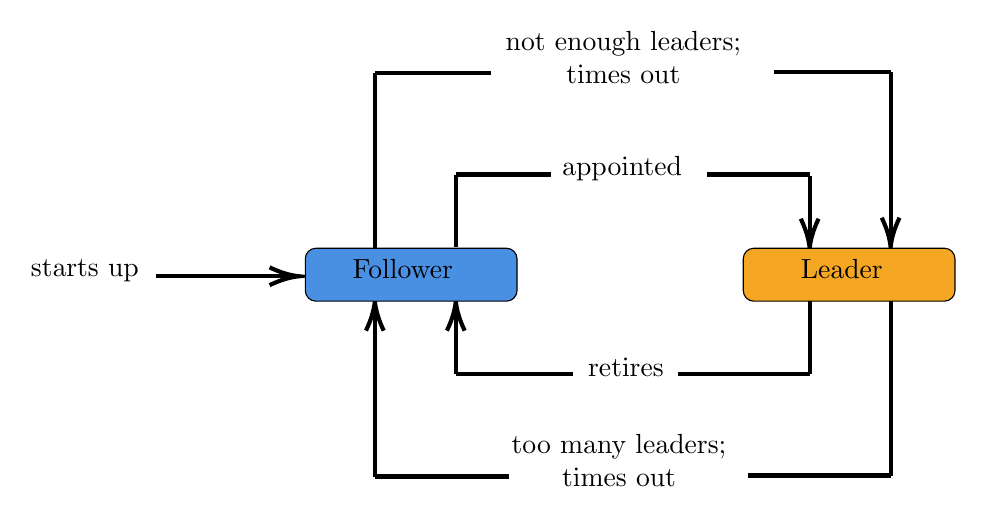
\begin{tikzpicture}[x=0.75pt,y=0.75pt,yscale=-1,xscale=1]
%uncomment if require: \path (0,300); %set diagram left start at 0, and has height of 300

%Straight Lines [id:da7582024624443486] 
\draw [line width=1.5]    (74.5,153.75) -- (140.5,153.75) ;
\draw [shift={(143.5,153.75)}, rotate = 180] [color={rgb, 255:red, 0; green, 0; blue, 0 }  ][line width=1.5]    (14.21,-4.28) .. controls (9.04,-1.82) and (4.3,-0.39) .. (0,0) .. controls (4.3,0.39) and (9.04,1.82) .. (14.21,4.28)   ;
%Straight Lines [id:da1737175708146408] 
\draw [line width=1.5]    (219,168.75) -- (219,200.75) ;
\draw [shift={(219,165.75)}, rotate = 90] [color={rgb, 255:red, 0; green, 0; blue, 0 }  ][line width=1.5]    (14.21,-4.28) .. controls (9.04,-1.82) and (4.3,-0.39) .. (0,0) .. controls (4.3,0.39) and (9.04,1.82) .. (14.21,4.28)   ;
%Straight Lines [id:da0069991711386795386] 
\draw [line width=1.5]    (180,168.75) -- (180,250.25) ;
\draw [shift={(180,165.75)}, rotate = 90] [color={rgb, 255:red, 0; green, 0; blue, 0 }  ][line width=1.5]    (14.21,-4.28) .. controls (9.04,-1.82) and (4.3,-0.39) .. (0,0) .. controls (4.3,0.39) and (9.04,1.82) .. (14.21,4.28)   ;
%Straight Lines [id:da7997009254563132] 
\draw [line width=1.5]    (219,104.75) -- (219,139.75) ;
%Straight Lines [id:da6517634793539615] 
\draw [line width=1.5]    (180,55.75) -- (180,140.25) ;
%Straight Lines [id:da9381133415973326] 
\draw [line width=1.5]    (389.5,137.25) -- (389.5,105.25) ;
\draw [shift={(389.5,140.25)}, rotate = 270] [color={rgb, 255:red, 0; green, 0; blue, 0 }  ][line width=1.5]    (14.21,-4.28) .. controls (9.04,-1.82) and (4.3,-0.39) .. (0,0) .. controls (4.3,0.39) and (9.04,1.82) .. (14.21,4.28)   ;
%Straight Lines [id:da20475050027342967] 
\draw [line width=1.5]    (428.5,136.75) -- (428.5,55.25) ;
\draw [shift={(428.5,139.75)}, rotate = 270] [color={rgb, 255:red, 0; green, 0; blue, 0 }  ][line width=1.5]    (14.21,-4.28) .. controls (9.04,-1.82) and (4.3,-0.39) .. (0,0) .. controls (4.3,0.39) and (9.04,1.82) .. (14.21,4.28)   ;
%Straight Lines [id:da6314202210947096] 
\draw [line width=1.5]    (389.5,200.75) -- (389.5,165.75) ;
%Straight Lines [id:da8469144916993987] 
\draw [line width=1.5]    (428.5,249.75) -- (428.5,165.25) ;
%Straight Lines [id:da6059987412847359] 
\draw [line width=1.5]    (219,104.75) -- (265,104.75) ;
%Straight Lines [id:da8345372265263031] 
\draw [line width=1.5]    (340,104.75) -- (389.5,104.75) ;
%Straight Lines [id:da759250238348591] 
\draw [line width=1.5]    (219,200.75) -- (275.5,200.75) ;
%Straight Lines [id:da004199534393038551] 
\draw [line width=1.5]    (326,200.75) -- (389.5,200.75) ;
%Straight Lines [id:da6463360435279583] 
\draw [line width=1.5]    (180,55.75) -- (236,55.75) ;
%Straight Lines [id:da9478179483720361] 
\draw [line width=1.5]    (372.5,55.25) -- (428.5,55.25) ;
%Straight Lines [id:da38872862853815515] 
\draw [line width=1.5]    (360,249.75) -- (428.5,249.75) ;
%Straight Lines [id:da9605862890532954] 
\draw [line width=1.5]    (180,250.25) -- (244.5,250.25) ;
%Rounded Rect [id:dp1761614463331822] 
\draw  [fill={rgb, 255:red, 74; green, 144; blue, 226 }  ,fill opacity=1 ] (146.5,145.35) .. controls (146.5,142.53) and (148.78,140.25) .. (151.6,140.25) -- (243.4,140.25) .. controls (246.22,140.25) and (248.5,142.53) .. (248.5,145.35) -- (248.5,160.65) .. controls (248.5,163.47) and (246.22,165.75) .. (243.4,165.75) -- (151.6,165.75) .. controls (148.78,165.75) and (146.5,163.47) .. (146.5,160.65) -- cycle ;

%Rounded Rect [id:dp11855608762791614] 
\draw  [fill={rgb, 255:red, 245; green, 166; blue, 35 }  ,fill opacity=1 ] (357.5,145.35) .. controls (357.5,142.53) and (359.78,140.25) .. (362.6,140.25) -- (454.4,140.25) .. controls (457.22,140.25) and (459.5,142.53) .. (459.5,145.35) -- (459.5,160.65) .. controls (459.5,163.47) and (457.22,165.75) .. (454.4,165.75) -- (362.6,165.75) .. controls (359.78,165.75) and (357.5,163.47) .. (357.5,160.65) -- cycle ;


% Text Node
\draw (384,144.5) node [anchor=north west][inner sep=0.75pt]   [align=left] {Leader};
% Text Node
\draw (168,144.5) node [anchor=north west][inner sep=0.75pt]   [align=left] {Follower};
% Text Node
\draw (13,144.5) node [anchor=north west][inner sep=0.75pt]   [align=left] {starts up};
% Text Node
\draw (236.5,34.25) node [anchor=north west][inner sep=0.75pt]   [align=left] {\begin{minipage}[lt]{92.96pt}\setlength\topsep{0pt}
\begin{center}
not enough leaders;\\times out
\end{center}

\end{minipage}};
% Text Node
\draw (269,94.5) node [anchor=north west][inner sep=0.75pt]   [align=left] {appointed};
% Text Node
\draw (279,192) node [anchor=north west][inner sep=0.75pt]   [align=left] {\begin{minipage}[lt]{31.08pt}\setlength\topsep{0pt}
\begin{center}
retires
\end{center}

\end{minipage}};
% Text Node
\draw (240.5,228.75) node [anchor=north west][inner sep=0.75pt]   [align=left] {\begin{minipage}[lt]{83.84pt}\setlength\topsep{0pt}
\begin{center}
too many leaders;\\times out
\end{center}

\end{minipage}};


\end{tikzpicture}


    \caption[Role Change State Machine]{The rules for role changes. A follower becomes a leader when it is appointed by a leader, or when it assumes leadership as too few leaders are present. A leader becomes a follower when it retires or when too many leaders are present.}
\end{figure}

There are two questions that guide the design of this mechanism:
\begin{enumerate*}
    \item ``When should a leader retire?'' and
    \item ``Which robot should it appoint as its successor?''.
\end{enumerate*}
We codify the answers to these questions as the \textbf{Retirement Policy} and the \textbf{Successor Identification Policy}.

An effective Retirement Policy would have a leader serve the optimal term length. Ideally, this means that a leader serves for as long as possible and no longer. If a leader's tenure is too long, then the quality of its localisation may degrade, and so would the quality of its ground truth pose estimates. Yet, if a leader's tenure is too short, then it will introduce needless role changes, which the rest of the group would need to handle, needlessly consuming extra computational resources.

An effective Successor Identification Policy would result in the appointment of the most suitable follower as a successor. One follower is more suitable than another if it can \begin{enumerate}
    \item Serve for more time.
    \item Provide better ground truth pose estimates.
    \item Serve more followers.
\end{enumerate}
However, designing a policy that achieves these goals is complicated, since each goal can be affected by many factors. For example, a follower with a higher quality localisation may serve for less time than another with a lower quality one, if it moves away from its followers.

After a leader has chosen a good successor, it would inform its successor about the change and subsequently resign. However, the successor cannot immediately assume leadership, as it could weaken the defences of the group. Successors are weakly-defended, meaning that they could be subtly biased. If then a biased successor were to be appointed leader, then that leader would itself be biased. Through contagion, this bias would slowly spread throughout the group. We prevent this problem by introducing a \textbf{transitory step} for successors. Before a successor can assume leadership, it must first reset its past localisations, to its leaders' beliefs. This ensures that the new leader is unbiased. 

\subsubsection{Exits, Mergers, and Acquisitions}
In Aegis, there are three important events that can occur. They are exits (when a robot leaves a group), mergers (when multiple mutually trusted groups encounter one another), and acquisitions (when a robot encounters a group that it trusts). We will now briefly discuss how the group will react to each of these events.

A robot may exit its group at any time. This may happen when the robot has physically moved away from the group and so cannot sense any of them, or it may happen if the robot suffers an internal fault. Regardless of the reason behind an exit, the group is largely unaffected. If the exiting robot is a leader, then it should instead appoint a successor before it leaves. Although this is not necessary, since the group will soon replace it. If instead, the exiting robot is a follower, then the group does not need to take action, since followers do not directly affect the group. After exiting, the follower would eventually observe that it has no leaders and appoint itself leader.

When multiple groups of robots merge, no action will be taken at first. Instead, the robots in the merged group would recognise that there are more leaders than needed. This would prompt some of the extraneous leaders to resign, thus restoring a healthy balance between leaders and followers.

In most circumstances where a group acquires a robot, the robot will be a leader, since individual robots can be thought of as ``groups of 1''. Since leaders are strongly-defended, the group does not need to directly take action. If acquiring a leader results in a surplus of leaders, then an extraneous leader will resign. There is one scenario where a group can acquire a follower, which is if the robot has just joined the RobotWeb. Here no action needs to be taken.

\subsection{A Proof of Correctness} \label{section:proof-correctness}
We will now formally prove the correctness of Aegis. It is correct if and only if \begin{enumerate*}
    \item leaders are strongly-defended, 
    \item followers are weakly-defended and
    \item the transitory step transforms a weakly-defended robot into a strongly-defended one.
\end{enumerate*}
\subsubsection{Leaders}
We consider a situation where the set of robots, $R$, is covered by the set of groups $GS$ and the set of attackers $A$, such that every robot in $R$ either belongs to a single group $G_i \in GS$ or is an attacker. Every group $G_i$ is covered by $L_i \cup F_i$ which refers to the leaders and followers in the group respectively. Since solitary robots act as leaders of groups of 1, $|F_i| = 1$.

At each iteration of the RobotWeb, a robot $r_i$ may send a message, $m_{ij}$ to $r_j$, where $m_{ij} := (\mu_{ij}, \Sigma_{ij}) = (\Lambda_{ij}^{-1}\eta_{ij}, \Lambda_{ij}^{-1})$.

We also define the following predicates:
\begin{align*}
    \mathbf{leader(r_i)} &\triangleq \exists{G_k \in GS}\left[r_i \in G_k \land r_i \in L_k\right]\\
    \mathbf{follower(r_i)} &\triangleq \exists{G_k \in GS}\left[r_i \in G_k \land r_i \in F_k\right]\\
    \mathbf{trusts(r_i, r_j)} &\triangleq leader(r_i) \implies (\exists{G \in GS}\left[r_i \in G \land r_j \in G\right] \land leader(r_j))\\
    \mathbf{accepts(r_i, m_{jk})} &\triangleq trusts(r_i, r_j)\\
    \mathbf{victim(r_i, r_a)} &\triangleq trusts(r_i, r_a) \lor \exists r_j \in R\left[trusts(r_i, r_j) \land victim(r_j, r_a)\right]
\end{align*}

Now in order to prove that leaders are \textbf{strongly-defended}, we must show that the following cannot hold:
\begin{equation}
    \exists r_i\in R, r_a \in A\left[leader(r_i) \land victim(r_i, r_a)\right]
\end{equation}
We take an arbitrary $r_i \in R$ and $r_a \in A$, such that $leader(r_i)$ holds. Now it is sufficient for us to prove that $victim(r_i, r_a)$ cannot hold.
\begin{align*}
    victim(r_i, r_a) \iff trusts(r_i, r_a) \lor \exists r_j \in R\left[trusts(r_i, r_j) \land victim(r_j, r_a)\right]
\end{align*}

First, we prove the left hand side cannot hold.
\begin{align*}
    trusts(r_i, r_a) &\iff leader(r_i) \implies (\exists{G \in GS}\left[r_i \in G \land r_a \in G\right] \land leader(r_a)) \tag*{\text{By the definition of trusts($r_i$, $r_j$)}}\\
    &\iff \exists{G \in GS}\left[r_i \in G \land r_a \in G\right] \land leader(r_a) \tag*{\text{By the assumption that leader($r_i$) holds}}\\\
    &\iff False \land False \tag*{\text{Since $\neg \exists G\in GS\left[r_a\in G\right]$}}\\
    &\iff False
\end{align*}

Then we prove that the right hand side also cannot hold, by taking an arbitrary $r_j \in R$. Since $trusts(r_i, r_j)$ must hold, $r_j$ must be a leader in the same group as $r_i$. However, now as $r_j$ is a leader and a victim of $r_a$, there must exist some other robot $r_k \in R$ that $r_j$ trusts and is a victim of $r_a$. Since $r_j$ trusts $r_k$, it must be another leader in the same group as $r_i$ and $r_j$, and so yet another robot $r_l$ must exist, that is trusted by $r_k$ and is a victim of $r_a$. This recursion continues ad infinitum, but since the number of leaders in a group is finite, this cannot be possible. Hence the right hand side also doesn't hold.

Since neither the left nor right hand sides hold, $victim(r_i, r_a)$ also cannot hold. Thus it is impossible for an attacker to influence a leader, and so leaders are well-defended.
\subsubsection{Followers}
Unlike leaders, followers can be influenced by attackers as they accept messages from all robots. Yet we can still prove that they are well-defended by proving that they will localise to points close to the ground truth, instead of the arbitrary points suggested by attackers. 

At each iteration of belief propagation, a follower will receive a set of messages $M$. These can be grouped into 2 distinct sets consisting of messages from its leaders, $M_l$, and other robots in the RobotWeb, $M_r$), where a subset, $M_a \subseteq M_r$, will be sent by attackers. The robot will first use \autoref{eqn:gbp-sum} to combine the leaders' messages into the baseline estimate, $N(\mu_l, \Sigma_l)$. Then it will measure the distance between each message $m_i \in M_r$ from $\mu_l$ and filter out any message $m_i = (\mu_i, \Sigma_i)$ where $||\mu_i - \mu_l||_2 > \epsilon$. Finally, it will combine all messages that passed through the filter and the leaders' messages, using \autoref{eqn:gbp-sum}, to compute its final belief, $(\mu, \Sigma)$. For an attack to be successful, the final belief must escape the $\epsilon$-bound, otherwise, the follower's localisation will always closely follow its ground truth pose. Formally, this means:

\begin{theorem}[Criteria for a Successful Attack]
\label{theo:successful-attack-criteria}
An attack can be considered to be successful if and only if there exists $M_a$ such that the final localisation $\mu$ of the attacked robot satisfies: \[\norm{\mu - \mu_l} > \epsilon \tag{where $\epsilon > 0$}\]
\end{theorem}

We will now prove that \ref{theo:successful-attack-criteria} cannot be satisfied.

Let $M_c$ represent the union between all the messages passed through the filter and the leaders' messages. We know that the following holds:
\begin{equation}
    \forall i \in M_c \left[ \norm{\mu_i - \mu_l} \leq \epsilon\right] \label{eqn:all_smaller}
\end{equation}

The Euclidean distance between the final localisation and the baseline estimate is:
\begin{align}
    \norm{\mu - \mu_l} &= \norm{\left(\sum_{i \in M_c} \left(\sum_{j \in M_c} \Lambda_j\right)^{-1} \eta_i\right)  - \mu_l} \tag*{\text{By \ref{eqn:gbp-sum}}}\\
    &= \norm{\left(\sum_{i \in M_c} \left(\sum_{j \in M_c} \Lambda_j\right)^{-1} \Lambda_i\mu_i\right)  - \mu_l} \tag*{\text{By \ref{eqn:canonical}}}
\end{align}

Now noticing that:
\begin{align}
    I &= A^{-1}A\\
      &= \left(\sum_{i \in M_c} \Lambda_i\right)^{-1}\left(\sum_{i \in M_c} \Lambda_i\right)\\
      &= \sum_{i \in M_c} \left(\sum_{j \in M_c} \Lambda_j\right)^{-1}\Lambda_i \label{eqn:sub}
\end{align}
We can substitute \autoref{eqn:sub} into the above expression for the Euclidean distance between the final localisation and baseline estimate to obtain:
\begin{align}
    \norm{\mu - \mu_l} &= \norm{\left(\sum_{i \in M_c} \left(\sum_{j \in M_c} \Lambda_j\right)^{-1} \Lambda_i\mu_i\right)  - I\mu_l}\\
    &= \norm{\left(\sum_{i \in M_c} \left(\sum_{j \in M_c} \Lambda_j\right)^{-1} \Lambda_i\mu_i\right)  - \left(\sum_{i \in M_c} \left(\sum_{j \in M_c} \Lambda_j\right)^{-1}\Lambda_i\right)\mu_l}\\
     &= \norm{\sum_{i \in M_c} \left(\sum_{j \in M_c} \Lambda_j\right)^{-1} \Lambda_i\left(\mu_i - \mu_l\right)}\\
     &\leq \sum_{i \in M_c} \norm{\left(\sum_{j \in M_c} \Lambda_j\right)^{-1} \Lambda_i\left(\mu_i - \mu_l\right)} \tag*{By the sub-additive property}\\
     &\leq \sum_{i \in M_c} \norm{\left(\sum_{j \in M_c} \Lambda_j\right)^{-1} \Lambda_i}\norm{\mu_i - \mu_l} \tag*{By the sub-multiplicative property}
\end{align}
Now that we have an upper bound on the distance, we can use \autoref{eqn:all_smaller} to simplify the second norm so we have:
\begin{align}
    \norm{\mu - \mu_l} &\leq \epsilon\sum_{i \in M_c} \norm{\left(\sum_{j \in M_c} \Lambda_j\right)^{-1} \Lambda_i}
\end{align}
So now it is sufficient to prove that:
\begin{align}
    \sum_{i \in M_c} \norm{\left(\sum_{j \in M_c} \Lambda_j\right)^{-1} \Lambda_i} \leq 1
\end{align}
To simplify the following equations we make the following substitution:
\begin{align}
    \Omega_i = \left(\sum_{j \in M_c} \Lambda_j\right)^{-1} \Lambda_i
\end{align}

As we are using the induced l2 matrix norm, the value of $\norm{A}$ for some matrix $A$ is equal to its largest singular value. If $A$ is a symmetric matrix, we can make a further simplification and say that $\norm{A} = \lambda_{max}(A)$ where $\lambda_{max}(A)$ is the largest eigenvalue of $A$.

The matrix $\Lambda_i$ is a precision matrix, and so is guaranteed to be symmetric positive definite. We know that the sums, inverses, and matrix products of symmetric positive definite matrices are also symmetric positive definite matrices, meaning that $\Omega_i$ is guaranteed to be symmetric positive definite.

So now $\norm{\Omega_i} = \lambda_{max}(\Omega_i)$, which allows us to use Weyl's Inequality about Perturbation \cite{weyls}, which gives us the following inequality:
\begin{equation}
    \lambda_{max}\left(\sum_{i \in M_c} \Omega_i\right) \leq \sum_{i \in M_c} \lambda_{max}(\Omega_i)
\end{equation}
And since $\Omega_i$ is positive definite, we can guarantee that each eigenvalue is greater than 0. This satisfies an equality condition derived in \cite{weyls_equality} allowing us to write:
\begin{align}
    \sum_{i \in M_c} \lambda_{max}(\Omega_i) &= \lambda_{max}\left(\sum_{i \in M_c} \Omega_i\right)\\
    &= \lambda_{max}(I) \tag*{\text{By \ref{eqn:sub}}}\\
    &= 1
\end{align}

Therefore:
\begin{align}
    \norm{\mu - \mu_l} &\leq \epsilon\sum_{i \in M_c} \norm{\left(\sum_{j \in M_c} \Lambda_j\right)^{-1} \Lambda_i}\\
    &= \epsilon \sum_{i \in M_c} \norm{\Omega_i}\\
    &= \epsilon
\end{align}

And thus \ref{theo:successful-attack-criteria} cannot hold.\\

\subsubsection{Transitory Step}
The transitory step forces a follower to reset its localisations to those suggested by its leaders. As we have seen before, attackers are unable to influence leaders' beliefs, and so cannot influence the follower's new localisations. This means that the follower is now strongly-defended.

\section{Evaluation} \label{section:eval-def}
Now we shall evaluate Aegis in the same simulated environment as before. Our goal here is to explore and understand how our solution performs. To do this, we will first perform three separate analyses to evaluate how well it performs when robots are under attack, when are no longer under attack, and when are not being attacked. 

\subsection{Experimental Setup}
Our experimental setup here shares many similarities with its predecessor in \autoref{section:attacker_experiments}. We still have a single attacker against $n$ normal robots. Our robots still move along and localise to predefined paths and our attackers still try to trick them into localising onto another path. Finally, we will use the same configurable parameters as detailed in \autoref{table:attack-expr-params}. We will also extend the robots' sensing range to cover the entire area, in order to keep a constant number of leaders throughout.

In addition to these parameters, we introduce several more aimed at configuring groups. They are listed below in \autoref{table:defence-expr-params}

%TODO: fix table
\begin{table}[!ht]
\centering
\resizebox{\textwidth}{!}{%
\begin{tabular}{|c|c|c|}
\hline
\textbf{Parameter}              & \textbf{Description}                                                                               & \textbf{Default Value} \\ \hline
Maximum Leader Divergence       & The maximum distance that an accepted message can be from the baseline estimate. & 0.01m                  \\ \hline
Leader Timeout                  & The maximum time that a robot can be leaderless without appointing itself as a leader.             & 5 ticks                \\ \hline
Minimum Leader Count            & The minimum number of leaders that a robot should observe.                                         & 1                      \\ \hline
Maximum Leader Count            & The maximum number of leaders that a robot should observe.                                         & 1                      \\ \hline
Retirement Policy               & The policy used by a leader to decide when it should retire.                                       & Random: $p = 0.1$                \\ \hline
Successor Identification Policy & The policy used by a leader to decide on a successor.                                              & Random                 \\ \hline
\end{tabular}%
}
\caption{The default parameters used to configure groups in these experiments}
\label{table:defence-expr-params}
\end{table}


\subsubsection{Path Design}
However, our current setup does also differ from its predecessor. Most notably, we choose to use more realistic paths. We consider a scenario where multiple robots are patrolling a miniaturised rainforest, to prevent illegal deforestation. If the robots notice any suspicious activity, they will alert the forest rangers of their locations, and the rangers will investigate. Now a logger who wishes to sabotage this system would attack the RobotWeb. Their attackers would try to distort the patrollers' localisations to keep the rangers from searching in a specific area. We present these paths in the below diagram. Note that we have shrunk the area of the rainforest down to a 1m by 1m grid, for ease of visualisation; in practice, this should not matter.

\begin{figure}[!h]
	\centering
	

\tikzset{every picture/.style={line width=0.75pt}} %set default line width to 0.75pt        

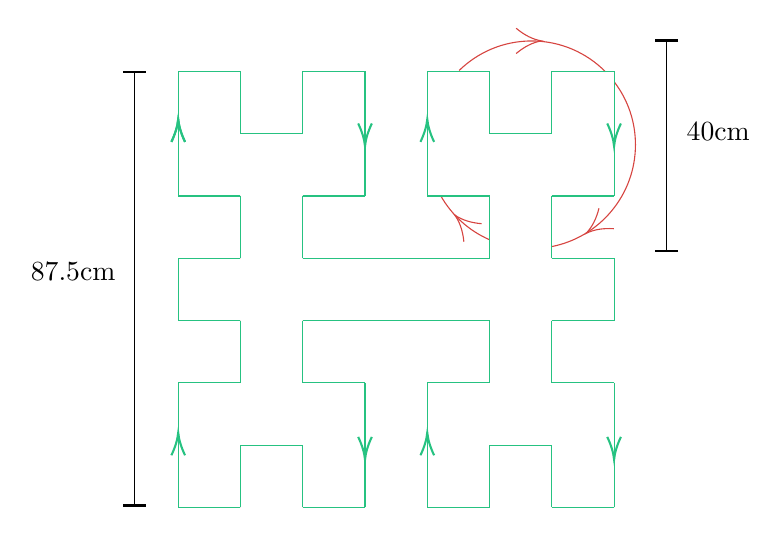
\begin{tikzpicture}[x=0.75pt,y=0.75pt,yscale=-1,xscale=1]
%uncomment if require: \path (0,300); %set diagram left start at 0, and has height of 300

%Shape: Arc [id:dp2186219161659576] 
\draw  [draw opacity=0] (380.97,43.57) .. controls (387.25,51.93) and (390.97,62.31) .. (390.97,73.57) .. controls (390.97,97.88) and (373.62,118.14) .. (350.62,122.64) -- (340.97,73.57) -- cycle ; \draw  [color={rgb, 255:red, 214; green, 69; blue, 65 }  ,draw opacity=1 ] (380.97,43.57) .. controls (387.25,51.93) and (390.97,62.31) .. (390.97,73.57) .. controls (390.97,97.88) and (373.62,118.14) .. (350.62,122.64) ;  
%Shape: Arc [id:dp14231683771998604] 
\draw  [draw opacity=0] (306.04,37.79) .. controls (315.05,28.99) and (327.38,23.57) .. (340.97,23.57) .. controls (354.86,23.57) and (367.44,29.24) .. (376.5,38.39) -- (340.97,73.57) -- cycle ; \draw  [color={rgb, 255:red, 214; green, 69; blue, 65 }  ,draw opacity=1 ] (306.04,37.79) .. controls (315.05,28.99) and (327.38,23.57) .. (340.97,23.57) .. controls (354.86,23.57) and (367.44,29.24) .. (376.5,38.39) ;  
%Shape: Arc [id:dp49745961484691537] 
\draw  [draw opacity=0] (320.55,119.3) .. controls (310.67,114.96) and (302.46,107.5) .. (297.16,98.18) -- (340.67,73.52) -- cycle ; \draw  [color={rgb, 255:red, 214; green, 69; blue, 65 }  ,draw opacity=1 ] (320.55,119.3) .. controls (310.67,114.96) and (302.46,107.5) .. (297.16,98.18) ;  

%Shape: Boxed Line [id:dp3721342518308307] 
\draw [color={rgb, 255:red, 38; green, 194; blue, 129 }  ,draw opacity=1 ][fill={rgb, 255:red, 174; green, 14; blue, 14 }  ,fill opacity=1 ]   (170.67,38.27) -- (200.67,38.27) ;
%Shape: Boxed Line [id:dp3172229534276627] 
\draw [color={rgb, 255:red, 38; green, 194; blue, 129 }  ,draw opacity=1 ][fill={rgb, 255:red, 174; green, 14; blue, 14 }  ,fill opacity=1 ]   (200.67,38.27) -- (200.67,68.27) ;
%Shape: Boxed Line [id:dp5212629188105563] 
\draw [color={rgb, 255:red, 38; green, 194; blue, 129 }  ,draw opacity=1 ][fill={rgb, 255:red, 174; green, 14; blue, 14 }  ,fill opacity=1 ]   (230.67,38.27) -- (230.67,68.27) ;
%Shape: Boxed Line [id:dp5675465040988046] 
\draw [color={rgb, 255:red, 38; green, 194; blue, 129 }  ,draw opacity=1 ][fill={rgb, 255:red, 174; green, 14; blue, 14 }  ,fill opacity=1 ]   (260.67,188.27) -- (230.67,188.27) ;
%Shape: Boxed Line [id:dp7202927705489535] 
\draw [color={rgb, 255:red, 38; green, 194; blue, 129 }  ,draw opacity=1 ][fill={rgb, 255:red, 174; green, 14; blue, 14 }  ,fill opacity=1 ]   (230.67,68.27) -- (200.67,68.27) ;
%Shape: Boxed Line [id:dp5092276311671151] 
\draw [color={rgb, 255:red, 38; green, 194; blue, 129 }  ,draw opacity=1 ][fill={rgb, 255:red, 174; green, 14; blue, 14 }  ,fill opacity=1 ]   (200.67,158.27) -- (200.67,188.27) ;
%Shape: Boxed Line [id:dp09856537256988473] 
\draw [color={rgb, 255:red, 38; green, 194; blue, 129 }  ,draw opacity=1 ][fill={rgb, 255:red, 174; green, 14; blue, 14 }  ,fill opacity=1 ]   (260.67,38.27) -- (230.67,38.27) ;
%Straight Lines [id:da9207201128217454] 
\draw [color={rgb, 255:red, 38; green, 194; blue, 129 }  ,draw opacity=1 ][fill={rgb, 255:red, 174; green, 14; blue, 14 }  ,fill opacity=1 ]   (170.67,38.27) -- (170.67,98.27) ;
\draw [shift={(170.67,61.27)}, rotate = 90] [color={rgb, 255:red, 38; green, 194; blue, 129 }  ,draw opacity=1 ][line width=0.75]    (10.93,-3.29) .. controls (6.95,-1.4) and (3.31,-0.3) .. (0,0) .. controls (3.31,0.3) and (6.95,1.4) .. (10.93,3.29)   ;
%Shape: Boxed Line [id:dp6135659357326062] 
\draw [color={rgb, 255:red, 38; green, 194; blue, 129 }  ,draw opacity=1 ][fill={rgb, 255:red, 174; green, 14; blue, 14 }  ,fill opacity=1 ]   (200.67,98.27) -- (170.67,98.27) ;
%Shape: Boxed Line [id:dp29987278620332025] 
\draw [color={rgb, 255:red, 38; green, 194; blue, 129 }  ,draw opacity=1 ][fill={rgb, 255:red, 174; green, 14; blue, 14 }  ,fill opacity=1 ]   (260.67,98.27) -- (230.67,98.27) ;
%Shape: Boxed Line [id:dp5645420723593432] 
\draw [color={rgb, 255:red, 38; green, 194; blue, 129 }  ,draw opacity=1 ][fill={rgb, 255:red, 174; green, 14; blue, 14 }  ,fill opacity=1 ]   (230.67,98.27) -- (230.67,128.27) ;
%Shape: Boxed Line [id:dp512796349122867] 
\draw [color={rgb, 255:red, 38; green, 194; blue, 129 }  ,draw opacity=1 ][fill={rgb, 255:red, 174; green, 14; blue, 14 }  ,fill opacity=1 ]   (200.67,98.27) -- (200.67,128.27) ;
%Shape: Boxed Line [id:dp08544200734686702] 
\draw [color={rgb, 255:red, 38; green, 194; blue, 129 }  ,draw opacity=1 ][fill={rgb, 255:red, 174; green, 14; blue, 14 }  ,fill opacity=1 ]   (200.67,128.27) -- (170.67,128.27) ;
%Shape: Boxed Line [id:dp007251344716708852] 
\draw [color={rgb, 255:red, 38; green, 194; blue, 129 }  ,draw opacity=1 ][fill={rgb, 255:red, 174; green, 14; blue, 14 }  ,fill opacity=1 ]   (260.67,128.27) -- (230.67,128.27) ;
%Shape: Boxed Line [id:dp372022468671378] 
\draw [color={rgb, 255:red, 38; green, 194; blue, 129 }  ,draw opacity=1 ][fill={rgb, 255:red, 174; green, 14; blue, 14 }  ,fill opacity=1 ]   (290.67,128.27) -- (260.67,128.27) ;
%Shape: Boxed Line [id:dp16802207181986673] 
\draw [color={rgb, 255:red, 38; green, 194; blue, 129 }  ,draw opacity=1 ][fill={rgb, 255:red, 174; green, 14; blue, 14 }  ,fill opacity=1 ]   (290.67,38.27) -- (320.67,38.27) ;
%Shape: Boxed Line [id:dp010741829406028525] 
\draw [color={rgb, 255:red, 38; green, 194; blue, 129 }  ,draw opacity=1 ][fill={rgb, 255:red, 174; green, 14; blue, 14 }  ,fill opacity=1 ]   (320.67,38.27) -- (320.67,68.27) ;
%Shape: Boxed Line [id:dp4930385694807232] 
\draw [color={rgb, 255:red, 38; green, 194; blue, 129 }  ,draw opacity=1 ][fill={rgb, 255:red, 174; green, 14; blue, 14 }  ,fill opacity=1 ]   (350.67,38.27) -- (350.67,68.27) ;
%Shape: Boxed Line [id:dp08350244380111804] 
\draw [color={rgb, 255:red, 38; green, 194; blue, 129 }  ,draw opacity=1 ][fill={rgb, 255:red, 174; green, 14; blue, 14 }  ,fill opacity=1 ]   (350.67,68.27) -- (320.67,68.27) ;
%Shape: Boxed Line [id:dp8705647795304325] 
\draw [color={rgb, 255:red, 38; green, 194; blue, 129 }  ,draw opacity=1 ][fill={rgb, 255:red, 174; green, 14; blue, 14 }  ,fill opacity=1 ]   (380.67,38.27) -- (350.67,38.27) ;
%Shape: Boxed Line [id:dp09487566903812439] 
\draw [color={rgb, 255:red, 38; green, 194; blue, 129 }  ,draw opacity=1 ][fill={rgb, 255:red, 174; green, 14; blue, 14 }  ,fill opacity=1 ]   (320.67,98.27) -- (290.67,98.27) ;
%Shape: Boxed Line [id:dp4467449565003223] 
\draw [color={rgb, 255:red, 38; green, 194; blue, 129 }  ,draw opacity=1 ][fill={rgb, 255:red, 174; green, 14; blue, 14 }  ,fill opacity=1 ]   (380.67,98.27) -- (350.67,98.27) ;
%Shape: Boxed Line [id:dp6555759862430016] 
\draw [color={rgb, 255:red, 38; green, 194; blue, 129 }  ,draw opacity=1 ][fill={rgb, 255:red, 174; green, 14; blue, 14 }  ,fill opacity=1 ]   (350.67,98.27) -- (350.67,128.27) ;
%Shape: Boxed Line [id:dp6429881015928276] 
\draw [color={rgb, 255:red, 38; green, 194; blue, 129 }  ,draw opacity=1 ][fill={rgb, 255:red, 174; green, 14; blue, 14 }  ,fill opacity=1 ]   (320.67,98.27) -- (320.67,128.27) ;
%Shape: Boxed Line [id:dp9933493383052265] 
\draw [color={rgb, 255:red, 38; green, 194; blue, 129 }  ,draw opacity=1 ][fill={rgb, 255:red, 174; green, 14; blue, 14 }  ,fill opacity=1 ]   (320.67,128.27) -- (290.67,128.27) ;
%Shape: Boxed Line [id:dp22629214701044487] 
\draw [color={rgb, 255:red, 38; green, 194; blue, 129 }  ,draw opacity=1 ][fill={rgb, 255:red, 174; green, 14; blue, 14 }  ,fill opacity=1 ]   (380.67,128.27) -- (350.67,128.27) ;
%Shape: Boxed Line [id:dp5605791797338285] 
\draw [color={rgb, 255:red, 38; green, 194; blue, 129 }  ,draw opacity=1 ][fill={rgb, 255:red, 174; green, 14; blue, 14 }  ,fill opacity=1 ]   (200.67,158.27) -- (170.67,158.27) ;
%Shape: Boxed Line [id:dp21107077729645585] 
\draw [color={rgb, 255:red, 38; green, 194; blue, 129 }  ,draw opacity=1 ][fill={rgb, 255:red, 174; green, 14; blue, 14 }  ,fill opacity=1 ]   (170.67,128.27) -- (170.67,158.27) ;
%Shape: Boxed Line [id:dp6037627685291229] 
\draw [color={rgb, 255:red, 38; green, 194; blue, 129 }  ,draw opacity=1 ][fill={rgb, 255:red, 174; green, 14; blue, 14 }  ,fill opacity=1 ]   (380.67,128.27) -- (380.67,158.27) ;
%Shape: Boxed Line [id:dp7248509663647659] 
\draw [color={rgb, 255:red, 38; green, 194; blue, 129 }  ,draw opacity=1 ][fill={rgb, 255:red, 174; green, 14; blue, 14 }  ,fill opacity=1 ]   (200.67,188.27) -- (170.67,188.27) ;
%Shape: Boxed Line [id:dp8948499643023982] 
\draw [color={rgb, 255:red, 38; green, 194; blue, 129 }  ,draw opacity=1 ][fill={rgb, 255:red, 174; green, 14; blue, 14 }  ,fill opacity=1 ]   (230.67,218.27) -- (200.67,218.27) ;
%Shape: Boxed Line [id:dp8316512065816155] 
\draw [color={rgb, 255:red, 38; green, 194; blue, 129 }  ,draw opacity=1 ][fill={rgb, 255:red, 174; green, 14; blue, 14 }  ,fill opacity=1 ]   (200.67,218.27) -- (200.67,248.27) ;
%Shape: Boxed Line [id:dp5466409181373546] 
\draw [color={rgb, 255:red, 38; green, 194; blue, 129 }  ,draw opacity=1 ][fill={rgb, 255:red, 174; green, 14; blue, 14 }  ,fill opacity=1 ]   (200.67,248.27) -- (170.67,248.27) ;
%Shape: Boxed Line [id:dp738241060404709] 
\draw [color={rgb, 255:red, 38; green, 194; blue, 129 }  ,draw opacity=1 ][fill={rgb, 255:red, 174; green, 14; blue, 14 }  ,fill opacity=1 ]   (230.67,218.27) -- (230.67,248.27) ;
%Shape: Boxed Line [id:dp8248899272473633] 
\draw [color={rgb, 255:red, 38; green, 194; blue, 129 }  ,draw opacity=1 ][fill={rgb, 255:red, 174; green, 14; blue, 14 }  ,fill opacity=1 ]   (260.67,248.27) -- (230.67,248.27) ;
%Shape: Boxed Line [id:dp4387660734130424] 
\draw [color={rgb, 255:red, 38; green, 194; blue, 129 }  ,draw opacity=1 ][fill={rgb, 255:red, 174; green, 14; blue, 14 }  ,fill opacity=1 ]   (260.67,158.27) -- (230.67,158.27) ;
%Shape: Boxed Line [id:dp09231026168318957] 
\draw [color={rgb, 255:red, 38; green, 194; blue, 129 }  ,draw opacity=1 ][fill={rgb, 255:red, 174; green, 14; blue, 14 }  ,fill opacity=1 ]   (230.67,158.27) -- (230.67,188.27) ;
%Shape: Boxed Line [id:dp004987953317974858] 
\draw [color={rgb, 255:red, 38; green, 194; blue, 129 }  ,draw opacity=1 ][fill={rgb, 255:red, 174; green, 14; blue, 14 }  ,fill opacity=1 ]   (290.67,158.27) -- (260.67,158.27) ;
%Shape: Boxed Line [id:dp3129885429495841] 
\draw [color={rgb, 255:red, 38; green, 194; blue, 129 }  ,draw opacity=1 ][fill={rgb, 255:red, 174; green, 14; blue, 14 }  ,fill opacity=1 ]   (320.67,158.27) -- (290.67,158.27) ;
%Shape: Boxed Line [id:dp3250621334664481] 
\draw [color={rgb, 255:red, 38; green, 194; blue, 129 }  ,draw opacity=1 ][fill={rgb, 255:red, 174; green, 14; blue, 14 }  ,fill opacity=1 ]   (320.67,188.27) -- (290.67,188.27) ;
%Shape: Boxed Line [id:dp6968262667370082] 
\draw [color={rgb, 255:red, 38; green, 194; blue, 129 }  ,draw opacity=1 ][fill={rgb, 255:red, 174; green, 14; blue, 14 }  ,fill opacity=1 ]   (320.67,158.27) -- (320.67,188.27) ;
%Shape: Boxed Line [id:dp9386922152430821] 
\draw [color={rgb, 255:red, 38; green, 194; blue, 129 }  ,draw opacity=1 ][fill={rgb, 255:red, 174; green, 14; blue, 14 }  ,fill opacity=1 ]   (350.67,158.27) -- (350.67,188.27) ;
%Shape: Boxed Line [id:dp8295491804817827] 
\draw [color={rgb, 255:red, 38; green, 194; blue, 129 }  ,draw opacity=1 ][fill={rgb, 255:red, 174; green, 14; blue, 14 }  ,fill opacity=1 ]   (380.67,158.27) -- (350.67,158.27) ;
%Shape: Boxed Line [id:dp9221615532737761] 
\draw [color={rgb, 255:red, 38; green, 194; blue, 129 }  ,draw opacity=1 ][fill={rgb, 255:red, 174; green, 14; blue, 14 }  ,fill opacity=1 ]   (380.67,188.27) -- (350.67,188.27) ;
%Shape: Boxed Line [id:dp24977202444232294] 
\draw [color={rgb, 255:red, 38; green, 194; blue, 129 }  ,draw opacity=1 ][fill={rgb, 255:red, 174; green, 14; blue, 14 }  ,fill opacity=1 ]   (320.67,218.27) -- (320.67,248.27) ;
%Shape: Boxed Line [id:dp07515950258992687] 
\draw [color={rgb, 255:red, 38; green, 194; blue, 129 }  ,draw opacity=1 ][fill={rgb, 255:red, 174; green, 14; blue, 14 }  ,fill opacity=1 ]   (320.67,248.27) -- (290.67,248.27) ;
%Shape: Boxed Line [id:dp9273354391230249] 
\draw [color={rgb, 255:red, 38; green, 194; blue, 129 }  ,draw opacity=1 ][fill={rgb, 255:red, 174; green, 14; blue, 14 }  ,fill opacity=1 ]   (350.67,218.27) -- (320.67,218.27) ;
%Shape: Boxed Line [id:dp24647337049235973] 
\draw [color={rgb, 255:red, 38; green, 194; blue, 129 }  ,draw opacity=1 ][fill={rgb, 255:red, 174; green, 14; blue, 14 }  ,fill opacity=1 ]   (350.67,218.27) -- (350.67,248.27) ;
%Shape: Boxed Line [id:dp9111717957922717] 
\draw [color={rgb, 255:red, 38; green, 194; blue, 129 }  ,draw opacity=1 ][fill={rgb, 255:red, 174; green, 14; blue, 14 }  ,fill opacity=1 ]   (380.67,248.27) -- (350.67,248.27) ;
\draw  [color={rgb, 255:red, 214; green, 69; blue, 65 }  ,draw opacity=1 ] (308.3,120.31) .. controls (307.78,115.05) and (306.31,110.74) .. (303.89,107.41) .. controls (307.26,109.77) and (311.59,111.18) .. (316.86,111.62) ;
\draw  [color={rgb, 255:red, 214; green, 69; blue, 65 }  ,draw opacity=1 ] (333.47,17.44) .. controls (337.53,20.83) and (341.6,22.86) .. (345.67,23.54) .. controls (341.6,24.22) and (337.53,26.25) .. (333.47,29.64) ;
\draw  [color={rgb, 255:red, 214; green, 69; blue, 65 }  ,draw opacity=1 ] (380.59,114.03) .. controls (375.31,113.69) and (370.83,114.45) .. (367.14,116.31) .. controls (370.03,113.36) and (372.11,109.31) .. (373.39,104.18) ;
%Straight Lines [id:da19528287212263684] 
\draw    (405.95,23.36) -- (405.95,124.55) ;
\draw [shift={(405.95,124.55)}, rotate = 270] [color={rgb, 255:red, 0; green, 0; blue, 0 }  ][line width=0.75]    (0,5.59) -- (0,-5.59)   ;
\draw [shift={(405.95,23.36)}, rotate = 270] [color={rgb, 255:red, 0; green, 0; blue, 0 }  ][line width=0.75]    (0,5.59) -- (0,-5.59)   ;
%Straight Lines [id:da3466920952873117] 
\draw    (149.55,38.56) -- (149.55,247.39) ;
\draw [shift={(149.55,247.39)}, rotate = 270] [color={rgb, 255:red, 0; green, 0; blue, 0 }  ][line width=0.75]    (0,5.59) -- (0,-5.59)   ;
\draw [shift={(149.55,38.56)}, rotate = 270] [color={rgb, 255:red, 0; green, 0; blue, 0 }  ][line width=0.75]    (0,5.59) -- (0,-5.59)   ;
%Straight Lines [id:da9207201128217454] 
\draw [color={rgb, 255:red, 38; green, 194; blue, 129 }  ,draw opacity=1 ][fill={rgb, 255:red, 174; green, 14; blue, 14 }  ,fill opacity=1 ]   (170.67,38.27) -- (170.67,98.27) ;
\draw [shift={(170.67,61.27)}, rotate = 90] [color={rgb, 255:red, 38; green, 194; blue, 129 }  ,draw opacity=1 ][line width=0.75]    (10.93,-3.29) .. controls (6.95,-1.4) and (3.31,-0.3) .. (0,0) .. controls (3.31,0.3) and (6.95,1.4) .. (10.93,3.29)   ;
%Straight Lines [id:da727447266636706] 
\draw [color={rgb, 255:red, 38; green, 194; blue, 129 }  ,draw opacity=1 ]   (260.67,38.27) -- (260.67,98.27) ;
\draw [shift={(260.67,74.27)}, rotate = 270] [color={rgb, 255:red, 38; green, 194; blue, 129 }  ,draw opacity=1 ][line width=0.75]    (10.93,-3.29) .. controls (6.95,-1.4) and (3.31,-0.3) .. (0,0) .. controls (3.31,0.3) and (6.95,1.4) .. (10.93,3.29)   ;
%Straight Lines [id:da8322774976347161] 
\draw [color={rgb, 255:red, 38; green, 194; blue, 129 }  ,draw opacity=1 ]   (290.67,38.27) -- (290.67,98.27) ;
\draw [shift={(290.67,61.27)}, rotate = 90] [color={rgb, 255:red, 38; green, 194; blue, 129 }  ,draw opacity=1 ][line width=0.75]    (10.93,-3.29) .. controls (6.95,-1.4) and (3.31,-0.3) .. (0,0) .. controls (3.31,0.3) and (6.95,1.4) .. (10.93,3.29)   ;
%Straight Lines [id:da9953290305227123] 
\draw [color={rgb, 255:red, 38; green, 194; blue, 129 }  ,draw opacity=1 ]   (380.67,38.27) -- (380.67,98.27) ;
\draw [shift={(380.67,74.27)}, rotate = 270] [color={rgb, 255:red, 38; green, 194; blue, 129 }  ,draw opacity=1 ][line width=0.75]    (10.93,-3.29) .. controls (6.95,-1.4) and (3.31,-0.3) .. (0,0) .. controls (3.31,0.3) and (6.95,1.4) .. (10.93,3.29)   ;
%Straight Lines [id:da3885684539910451] 
\draw [color={rgb, 255:red, 38; green, 194; blue, 129 }  ,draw opacity=1 ]   (170.67,248.27) -- (170.67,188.27) ;
\draw [shift={(170.67,212.27)}, rotate = 90] [color={rgb, 255:red, 38; green, 194; blue, 129 }  ,draw opacity=1 ][line width=0.75]    (10.93,-3.29) .. controls (6.95,-1.4) and (3.31,-0.3) .. (0,0) .. controls (3.31,0.3) and (6.95,1.4) .. (10.93,3.29)   ;
%Straight Lines [id:da2410496204005277] 
\draw [color={rgb, 255:red, 38; green, 194; blue, 129 }  ,draw opacity=1 ]   (260.67,248.27) -- (260.67,188.27) ;
\draw [shift={(260.67,225.27)}, rotate = 270] [color={rgb, 255:red, 38; green, 194; blue, 129 }  ,draw opacity=1 ][line width=0.75]    (10.93,-3.29) .. controls (6.95,-1.4) and (3.31,-0.3) .. (0,0) .. controls (3.31,0.3) and (6.95,1.4) .. (10.93,3.29)   ;
%Straight Lines [id:da06847277642029848] 
\draw [color={rgb, 255:red, 38; green, 194; blue, 129 }  ,draw opacity=1 ]   (380.67,248.27) -- (380.67,188.27) ;
\draw [shift={(380.67,225.27)}, rotate = 270] [color={rgb, 255:red, 38; green, 194; blue, 129 }  ,draw opacity=1 ][line width=0.75]    (10.93,-3.29) .. controls (6.95,-1.4) and (3.31,-0.3) .. (0,0) .. controls (3.31,0.3) and (6.95,1.4) .. (10.93,3.29)   ;
%Straight Lines [id:da22234560552897487] 
\draw [color={rgb, 255:red, 38; green, 194; blue, 129 }  ,draw opacity=1 ]   (290.67,248.27) -- (290.67,188.27) ;
\draw [shift={(290.67,212.27)}, rotate = 90] [color={rgb, 255:red, 38; green, 194; blue, 129 }  ,draw opacity=1 ][line width=0.75]    (10.93,-3.29) .. controls (6.95,-1.4) and (3.31,-0.3) .. (0,0) .. controls (3.31,0.3) and (6.95,1.4) .. (10.93,3.29)   ;

% Text Node
\draw (414.41,61.72) node [anchor=north west][inner sep=0.75pt]   [align=left] {40cm};
% Text Node
\draw (98.41,129.05) node [anchor=north west][inner sep=0.75pt]   [align=left] {87.5cm};


\end{tikzpicture}


	\caption[Paths used to evaluate defences]{An example of the types of paths we use to evaluate our defences. In this example, the robots will move along the green path, whilst attackers aim to trick them into localising onto the red path. Note that these paths have significant overlap, which hides much of the attacker's path.}
\end{figure}

Here the patrollers move along the green path, whilst the attackers aim to force them to localise to the red path. Note that the attackers only attack the patrollers when they approach the loggers' area. We can also see that paths have an ``onramping'' effect, where the patrollers would be slowly cajoled off their actual paths and onto alternative paths. The challenge for the patrollers is to ensure that they do not localise onto the attackers' path.

\subsubsection{Evaluation Metrics}
Since the actual and attacker's paths frequently overlap, we cannot use the ATE to measure the efficacy of our defence, as it is no longer a good metric. The reason for this is that a robot is only attacked when it is on a particular segment of its trajectory, whilst the ATE would measure the quality of its localisation across its entire trajectory. We solve this by calculating two ATEs; one when the robot is being attacked and one when it is not. The ATE when the robot is being attacked can be thought of as a measure of the \textit{resistance} of our defence, while the other ATE can be thought of as a measure of the \textit{resilience} of our defence. We will also evaluate Aegis in scenarios where it is not being attacked, to gain an understanding of the costs of using it. For each of these three metrics, a lower value indicates better performance.

If a robot can be easily tricked by an attacker, but after the attack quickly relocalises to its actual pose, then we can say that it has a low resistance but high resilience. Similarly, a robot that is largely unaffected during an attack, but suffers from a worse localisation after, can be thought of as having a high resistance but low resilience. Ideally, our defence will have both high resistance and resilience whilst having a low cost.

\subsection{Defence against Attacks}
Now we will evaluate the resistance and resilience of our defence when the group is being attacked, when a robot is under attack. Here we believe that defended robots will significantly outperform their undefended counterparts in both resistance and resilience.

\subsubsection{Overconfidence Attacks should be Ineffective}
We will start our experiments using overconfidence attacks when attackers present significantly higher confidence levels in order to influence their victims. We should observe that defended robots successfully resist these attacks. We test this by varying the confidence of the attacker and measuring the group's resistance and resilience. We also run this experiment without defences in order to discern the effect of our defences. We repeat this experiment 10 times.

\begin{figure}[!h]
	\centering
	\subfigure[Resistance: With defences]{
		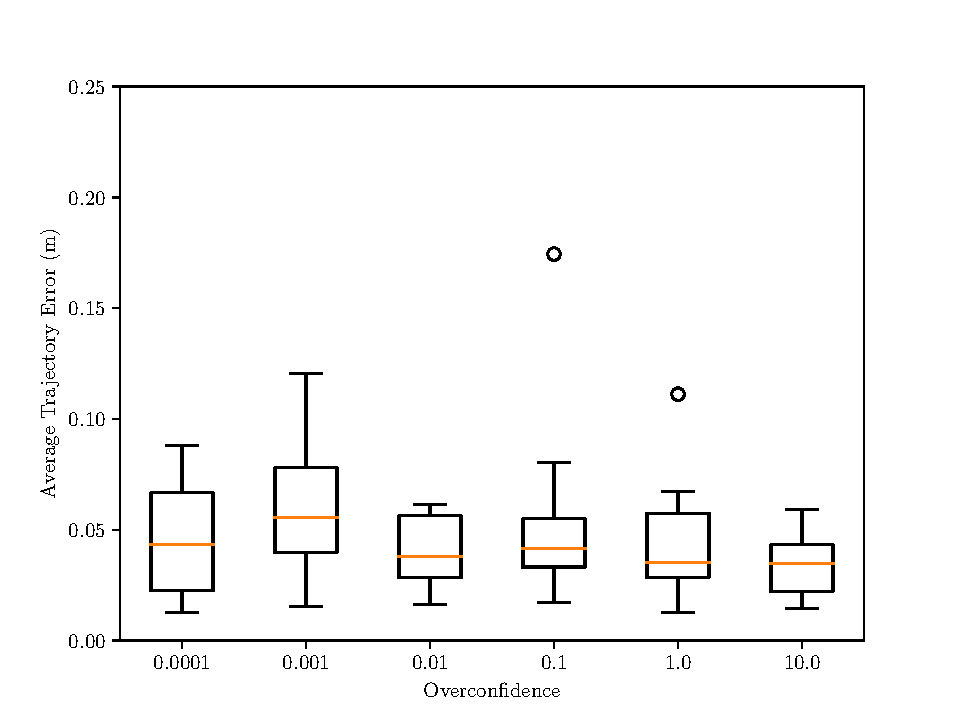
\includegraphics[width=0.45\textwidth]{report/graphs/wartime_overconfidence_resistance_defended.pdf}
		\label{fig:wartime-resistance-defended-overconf}
	}
	\subfigure[Resistance: Without defences]{
		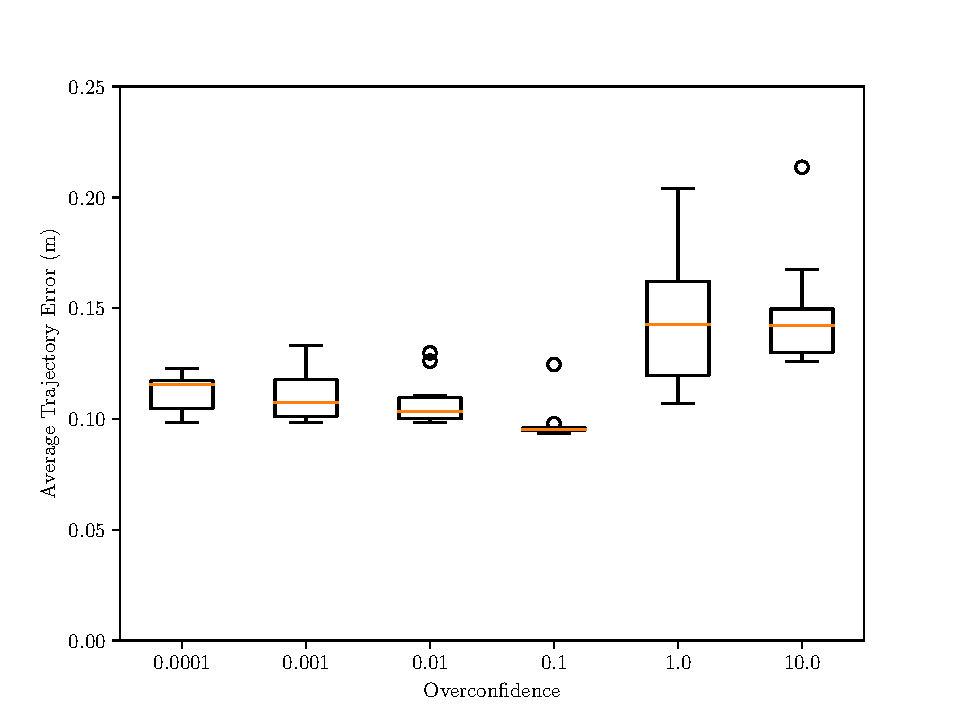
\includegraphics[width=0.45\textwidth]{report/graphs/wartime_overconfidence_resistance_undefended.pdf}
		\label{fig:wartime-resistance-undefended-overconf}
	}
 	\subfigure[Resilience: With defences]{
		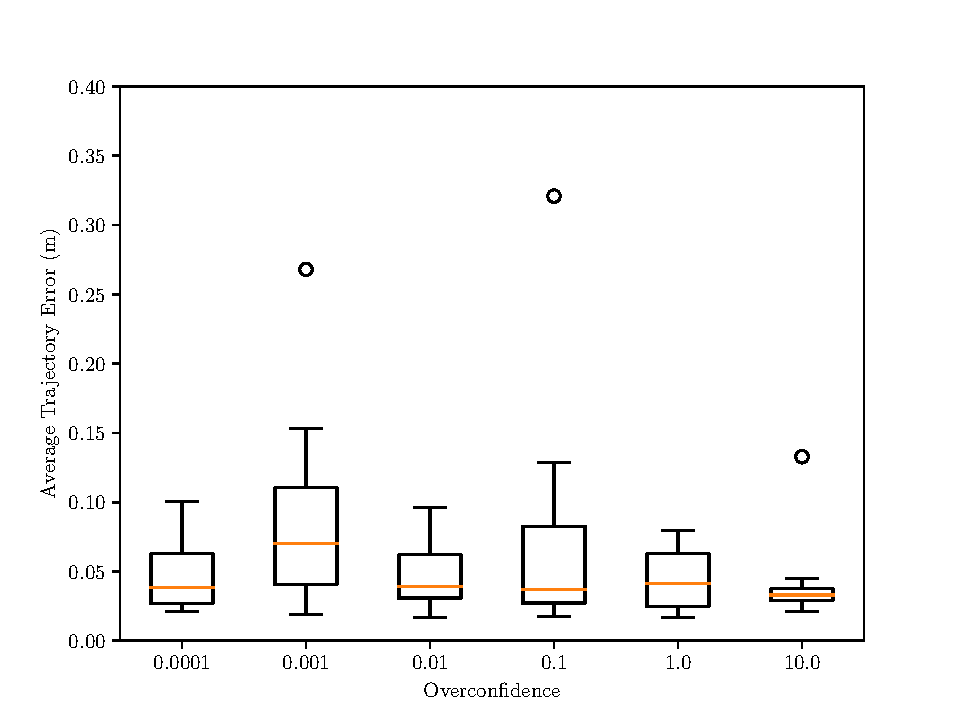
\includegraphics[width=0.45\textwidth]{report/graphs/wartime_overconfidence_resilience_defended.pdf}
		\label{fig:wartime-resilience-defended-overconf}
	}
	\subfigure[Resilience: Without defences]{
		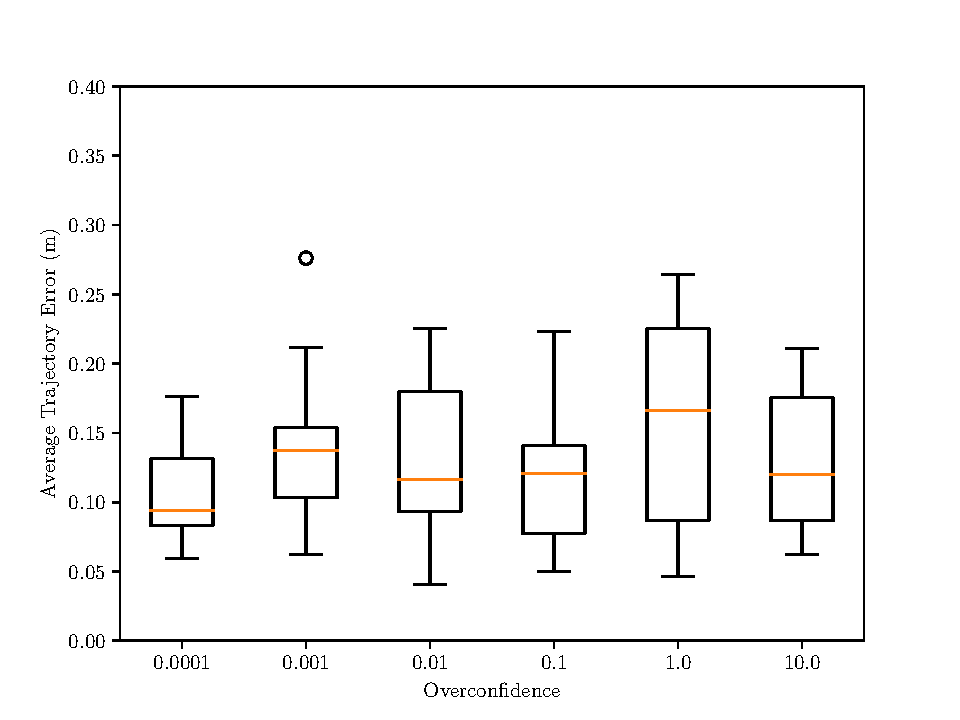
\includegraphics[width=0.45\textwidth]{report/graphs/wartime_overconfidence_resilience_undefended.pdf}
		\label{fig:wartime-resilience-undefended-overconf}
	}
	\caption{Aegis' resistance to and resilience against overconfidence attacks}
        \label{fig:wartime-overconf}
\end{figure}

From \autoref{fig:wartime-overconf}, we make several interesting observations. Firstly, we can see that the resilience of Aegis is worse than its resistance, yet this is likely due to a data imbalance since the group spends less time resisting attacks and more time recovering. We also obtain experimental confirmation that Aegis does successfully protect a group from overconfidence attacks, even as the strength of the attacks increases.

\begin{figure}[!h]
	\centering
	\subfigure[With defences]{
		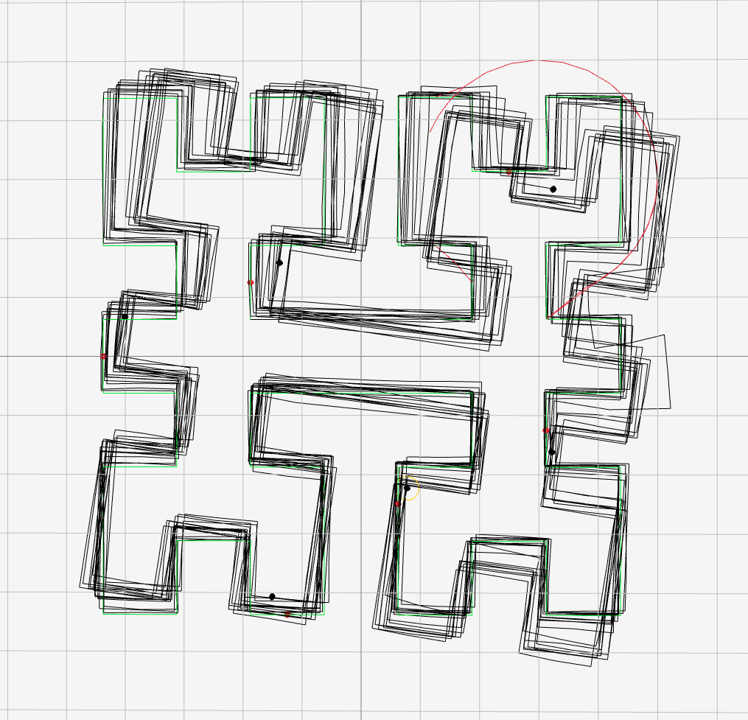
\includegraphics[width=0.45\textwidth]{report/diagrams/defence.png}
	}
	\subfigure[Without defences]{
		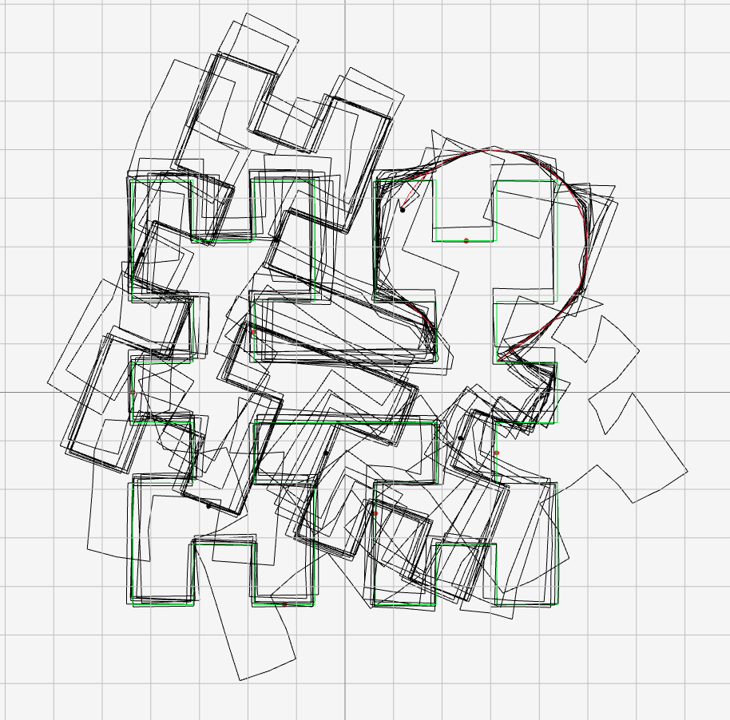
\includegraphics[width=0.45\textwidth]{report/diagrams/undefence.png}
	}
	\caption{Screenshots from the RobotWeb simulator showing the effect of running Aegis. Here the setup is the same as the above experiment and the attacker uses an overconfidence value of 0.01.}
        \label{fig:wartime-overconf}
\end{figure}

\subsubsection{Sybil Attacks should be Ineffective}
Now we repeat the above experiment, but this time using a Sybil attacker. Theoretically, the results of this experiment should match the results of the previous one, however, it is still important to experimentally confirm this. We vary the number of false identities that an attacker can create and measure the group's resistance and resilience. Again we compare this to a scenario without defences, repeating both 10 times. 

\begin{figure}[!h]
	\centering
	\subfigure[Resistance: With defences]{
		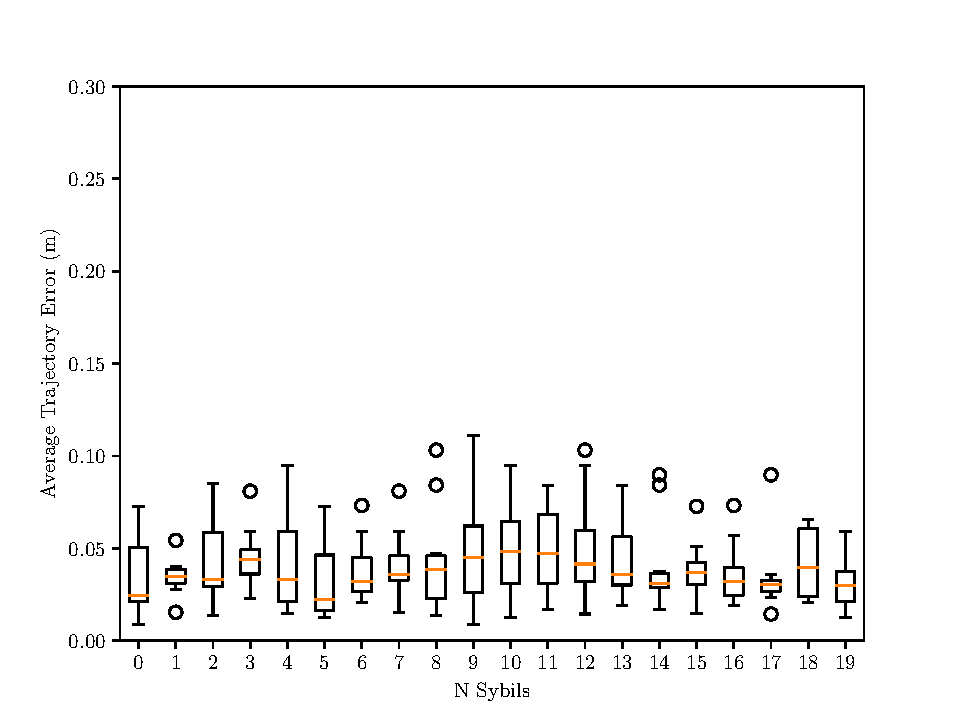
\includegraphics[width=0.45\textwidth]{report/graphs/wartime_sybils_resistance_defended.pdf}
		\label{fig:wartime-defended-resistance-sybil}
	}
	\subfigure[Resistance: Without defences]{
		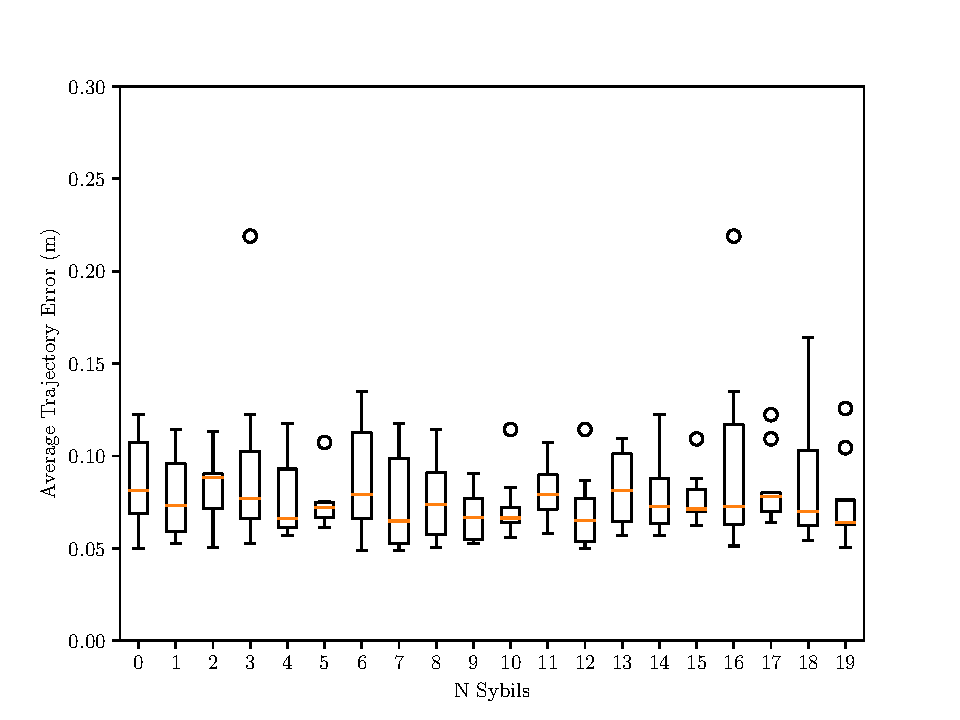
\includegraphics[width=0.45\textwidth]{report/graphs/wartime_sybils_resistance_undefended.pdf}
		\label{fig:wartime-undefended-resistance-sybil}
	}
 	\subfigure[Resilience: With defences]{
		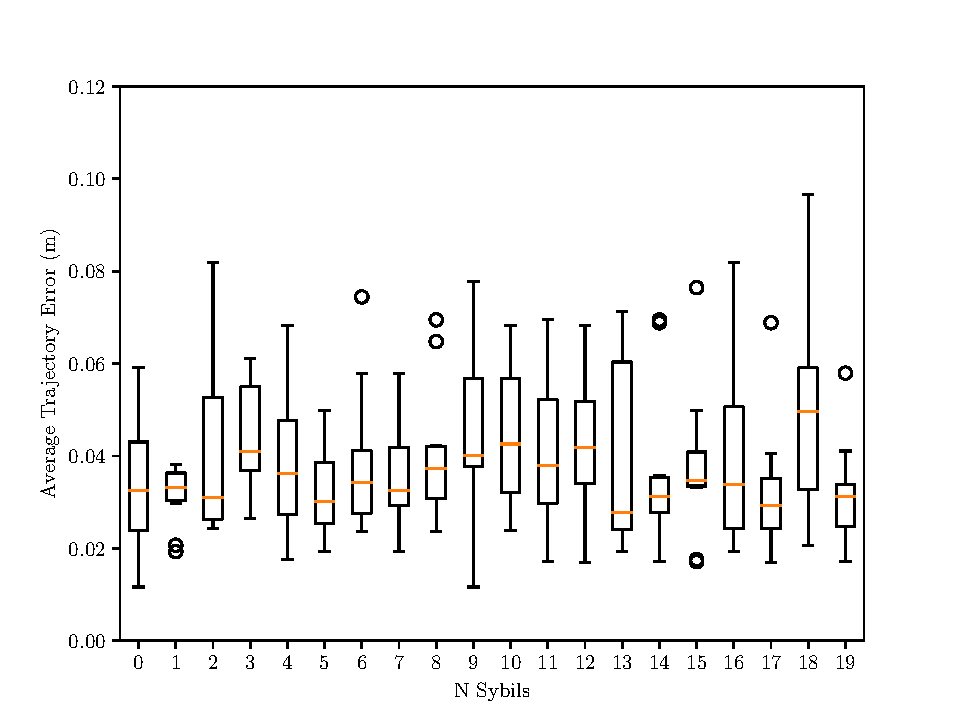
\includegraphics[width=0.45\textwidth]{report/graphs/wartime_sybils_resilience_defended.pdf}
		\label{fig:wartime-defended-resilience-sybil}
	}
	\subfigure[Resilience: Without defences]{
		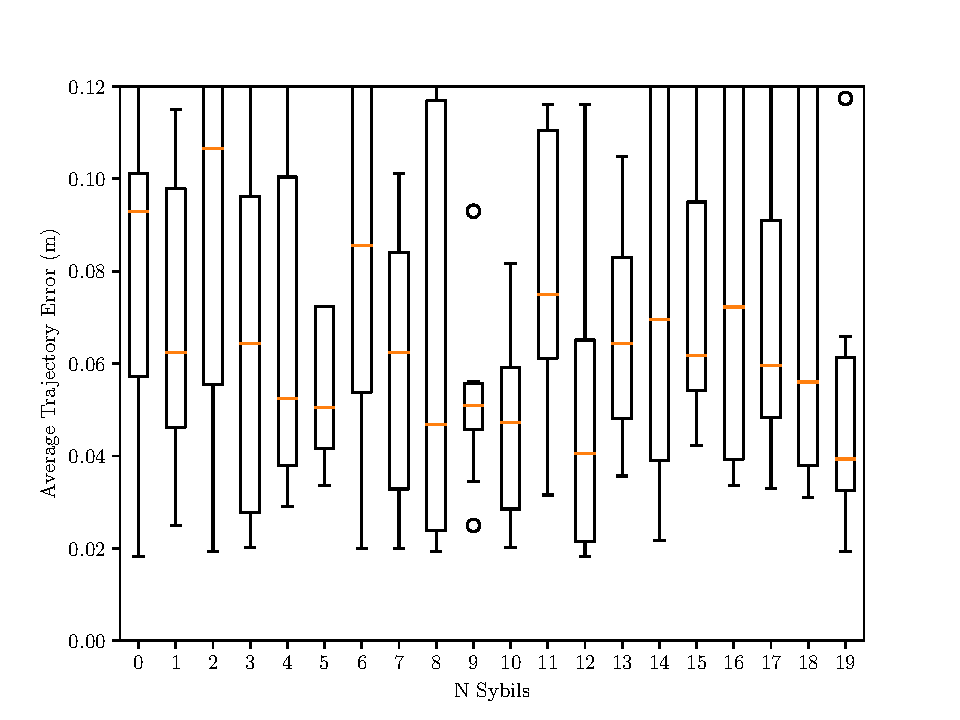
\includegraphics[width=0.45\textwidth]{report/graphs/wartime_sybils_resilience_undefended.pdf}
		\label{fig:wartime-undefended-resilience-sybil}
	}
	\caption{Aegis' resistance to and resilience against Sybil attacks}
         \label{fig:wartime-sybils}
\end{figure}

Again in \autoref{fig:wartime-sybils} we see that the resistance of Aegis is superior to its resilience. We also see that Aegis is resistant against Sybil attacks.

% \subsubsection{Are many groups better than one?}
% Finally, we test whether there is a benefit to using smaller more fragmented groups over larger groups. If there is such a benefit

% We keep the total number of robots constant but vary the number of groups in the simulation. For convenience, we form groups out of adjacent robots. 


% Almost finally, we'll do a bit of a weird one. We'll see how multiple groups interact with one another. We'll keep the total number of robots constant, but vary the number of groups. For convenience, robots near each other on the path will form groups. This might be kinda sus, since we're also changing the group sizes, but if we kept the group size constant, we're also changing the number of robots in total. What we're really getting at though is the relationship between number of robots and the number of groups. Is it better to have more groups or more robots. If it turns out (prolly won't) that more groups is better, then it'll be better for real peeps to have smaller groups. We'll measure perf vs n groups and repeat 10x.

\subsection{Defence when no Attackers are Present}
Now we will evaluate the ATE of Aegis, when no attackers are present. We expect that defended robots will have a slightly higher ATE than undefended robots. The reason behind this is that undefended robots are able to participate more than defended robots since they \begin{enumerate*}
    \item do not reject any messages and
    \item have no leaders which are isolated from the RobotWeb
\end{enumerate*}, which should allow them to reap more of the benefits of participation.

We measure the cost of defence by running the simulation both with and without defences, repeating this 10 times.
\begin{figure}[!h]
	\centering
        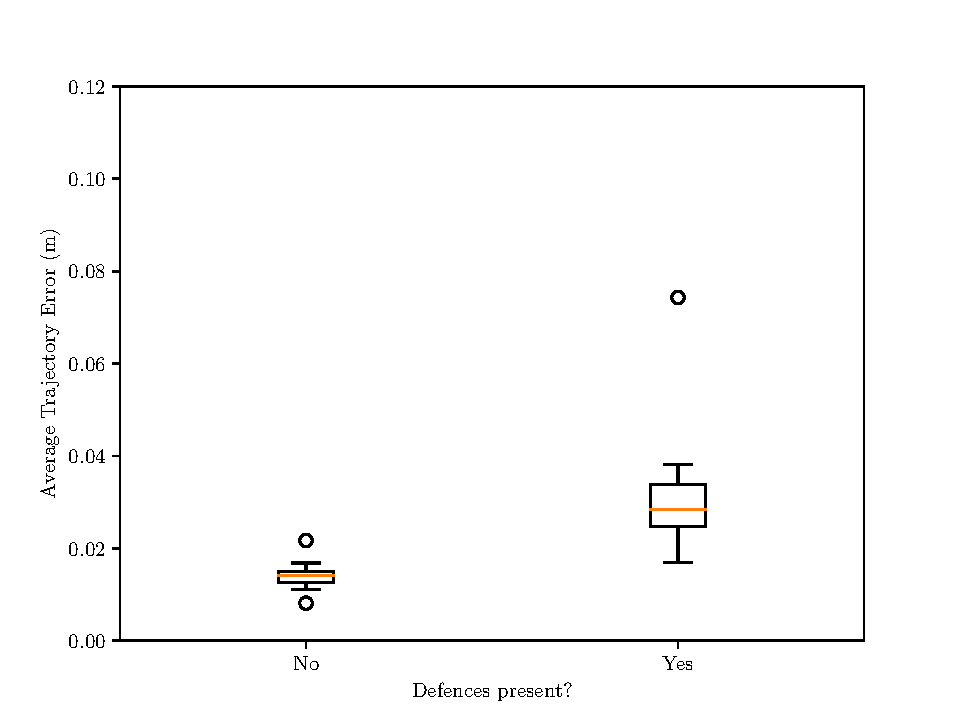
\includegraphics[width=7cm]{report/graphs/peacetime.pdf}
	\caption{The cost of using defences when no attackers are present.}
        \label{fig:peacetime}
\end{figure}

Now from \autoref{fig:peacetime}, we can see that running Aegis does incur a performance penalty when no attackers are present. In fact, we can see that the addition of Aegis, almost doubles the ATE of robots. This is in line with our expectations as defended robots participate less in the RobotWeb, and so reap fewer of its benefits. Here no leader has any compatriots, and so they are essentially isolated, increasing their ATE, whilst their followers rely upon these worsened messages.

However, the decrease in performance is still quite small in absolute terms as it translates to an additional 0.015m of ATE. It is for this reason that we do not believe that the cost of Aegis is prohibitive to its usage.

Most importantly, if we compare these results to \autoref{fig:wartime-overconf} and \autoref{fig:wartime-sybils}, we see that the ATE when attackers are present is the same as when attackers are absent, once more experimentally confirming the potency of Aegis.

\subsubsection{Measuring the Effect of Multiple Groups}
In the above experiments, we only considered a single group, however in a real-world setting Aegis is likely to run on multiple groups, which mutually distrust one another. We will now briefly consider the effect including multiple groups, and varying their sizes, will have upon the performance of Aegis.

We will vary the size of the groups from 1 to 4, and also vary the number of groups from 1 to 4.
\begin{figure}[!h]
	\centering
	\subfigure[Resistance]{
		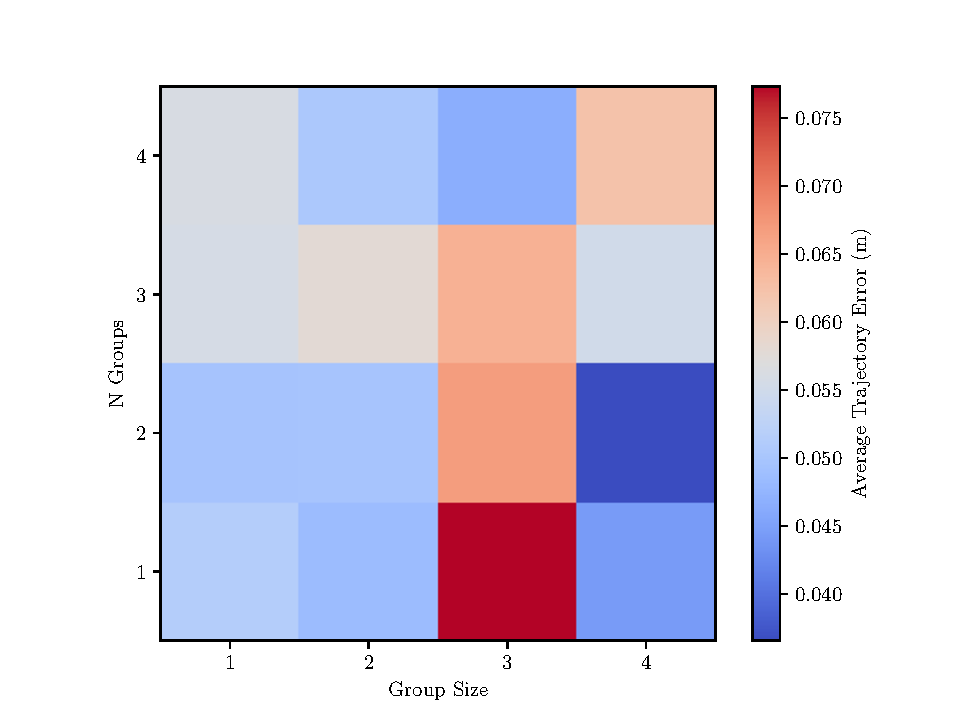
\includegraphics[width=0.3\textwidth]{report/graphs/n_groups_resistance.pdf}
		\label{fig:n-groups-resistance}
	}
	\subfigure[Resilience]{
		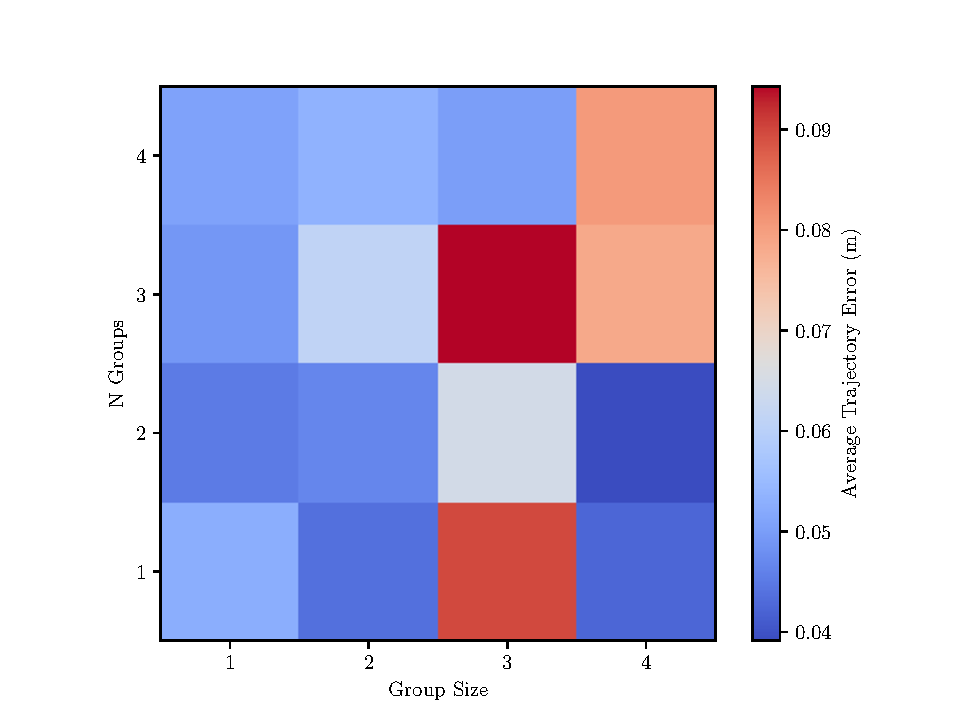
\includegraphics[width=0.3\textwidth]{report/graphs/n_groups_resilience.pdf}
		\label{fig:n-groups-resilience}
	}
 	\subfigure[Cost of Operation]{
		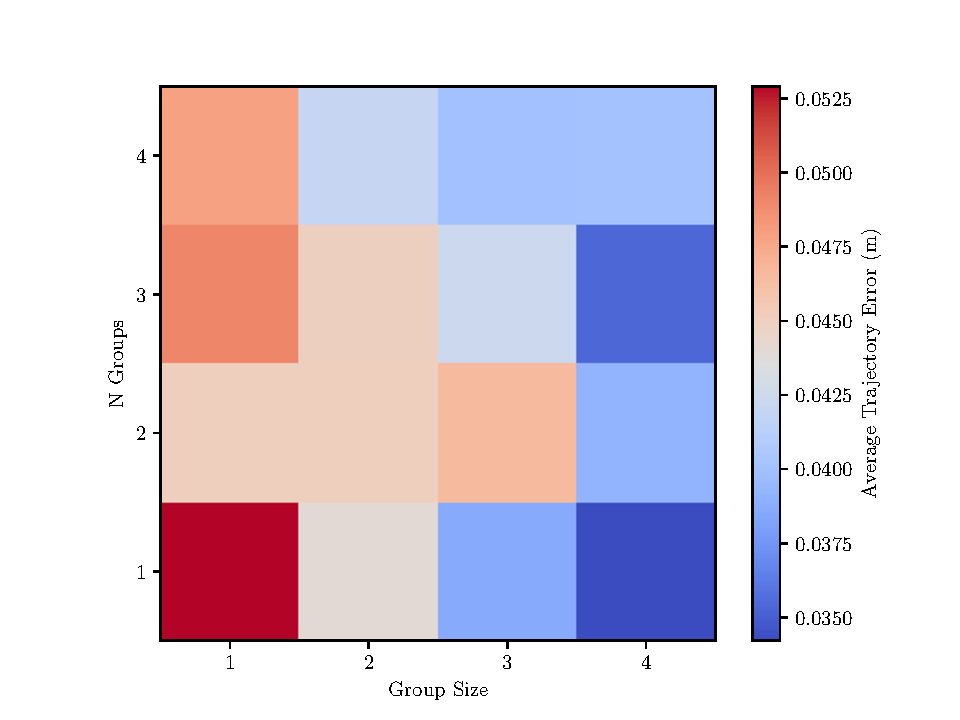
\includegraphics[width=0.3\textwidth]{report/graphs/n_groups_reduction.pdf}
		\label{fig:n-groups-reduction}
	}
	\caption{Varying the number of groups and the overall group sizes.}
\end{figure}

Examining \autoref{fig:n-groups-resistance} and \autoref{fig:n-groups-resilience}, we see no pattern in the performance, but we do see a markedly worse performance when the group size is 3, however, we do not believe that this effect is inherent to Aegis, instead it is likely to be a combination of the quirks of the environment and particular set of parameters used in this experiment. Now looking at the cost of operation, \autoref{fig:n-groups-reduction}, we see that increasing the number of groups does lead to a marked increase in the overall performance, as does increasing the group size. Furthermore, looking at the diagonals, we can see that increasing the size of a group leads to a lower cost than increasing the number of groups, which is likely due to the fact that robots inside a group have the guarantee of mutual trust, and so do not tend to reject one another's messages.

\subsection{Tuning the Parameters of Aegis} \label{section:optim}
In the previous sections, we used random policies and an arbitrary set of parameters to evaluate Aegis, yet these are unlikely to produce the best performance. Firstly, it is likely that a more carefully crafted Successor Identification or Retirement Policy would outperform a random policy. Secondly, it is also likely that varying both the minimum and maximum number of leaders in a group would have an effect on performance. Finally, it is also likely that the \textit{leader divergence} - $\epsilon$, plays a significant role in the final performance outcome.

We will now test these claims by comparing the performances of several alternative policies as well as by varying the aforementioned parameters. We will evaluate these when the group is both under attack and safe, in order to gain a holistic understanding of its strength, and costs.

A challenge that arises here, is that it is difficult to judge the relative weightings between these two situations. Firstly, because we have no data to indicate how often a robot should expect to be attacked. Secondly, we also cannot reliably estimate how harmful an attack would be, since this varies across use cases. We resolve this problem by not resolving it - we will instead compare the resistance, resilience and cost of operation, separately. We believe that this allows for a deeper understanding of the performance characteristics of our defence than a single value would, and thus be of greater decision-making value.

\subsubsection{Comparing different Retirement Policies}
We compare the random retirement policy with two new ones - a Fixed-Term Retirement Policy (FTRP) and a Confidence-Based Retirement Policy (CBRP). All three of these policies have their own configurable parameters, hence we must find their optimal parameters before we can compare them with one another.

In a random retirement policy, a leader can resign at any tick, with probability $p$. To find the best possible random retirement policy, we must find the optimal value of $p$. We do this by varying $p$ from 0.1 to 1, in increments of 0.1.
\begin{figure}[!h]
	\centering
	\subfigure[Resistance]{
		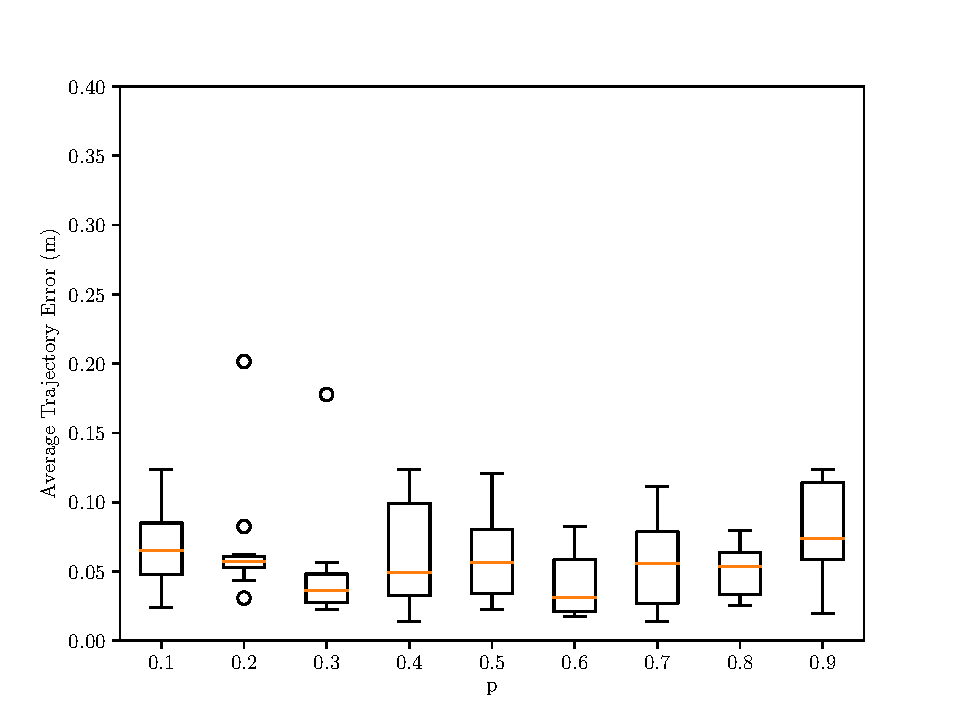
\includegraphics[width=0.3\textwidth]{report/graphs/random_resistance.pdf}
		\label{fig:random-resistance}
	}
	\subfigure[Resilience]{
		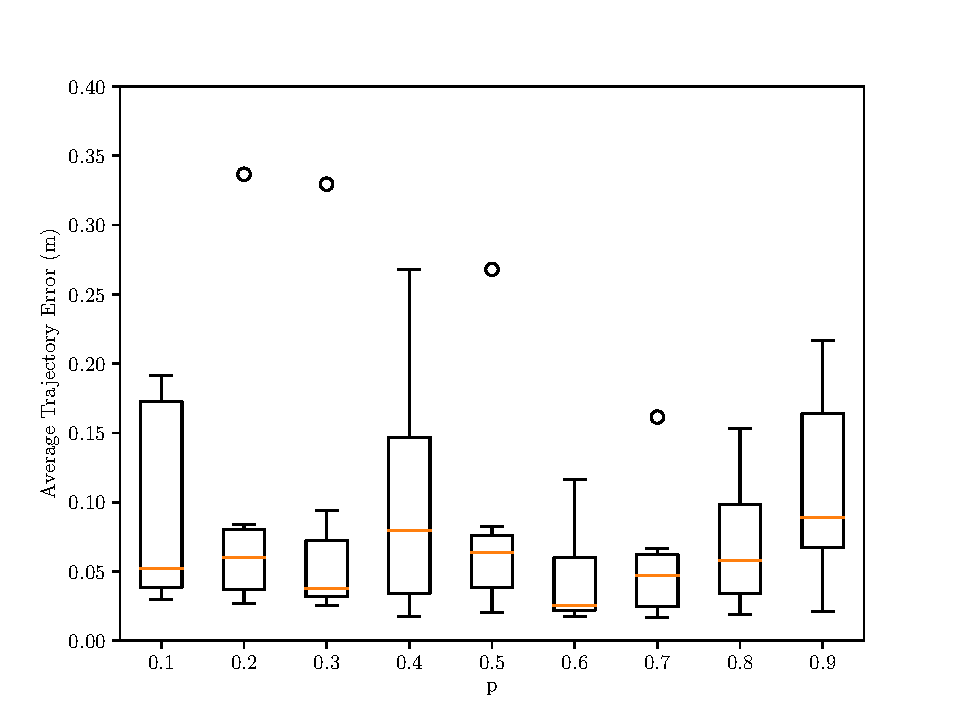
\includegraphics[width=0.3\textwidth]{report/graphs/random_resilience.pdf}
		\label{fig:random-resilience}
	}
 	\subfigure[Cost of Operation]{
		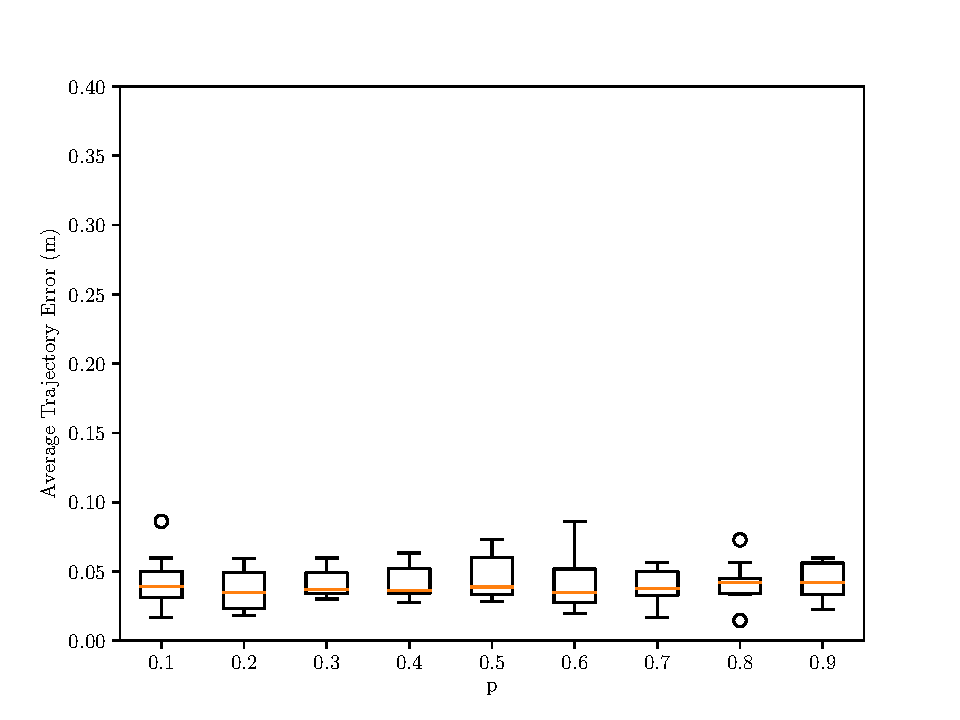
\includegraphics[width=0.3\textwidth]{report/graphs/random_reduction.pdf}
		\label{fig:random-reduction}
	}
	\caption{Finding the optimal value of $p$ for a random retirement policy}
        \label{fig:random}
\end{figure}

Looking at \label{fig:random}, we see no correlation between the probability of retirement, $p$, and the overall performance of Aegis. However, we do see a slight preference towards $p = 0.5$, when looking at the resilience, \autoref{fig:random-resilience}, which translates to an expected term length of 2. Yet we do not observe the same effect when using a FTRP in \autoref{fig:fixed-resilience}. This leads us to suspect that either all random policies are equal, or that more comprehensive experimentation is needed to truly measure its effect.

In a FTRP, leaders will retire after serving for a fixed, term length, $t$. We now vary the value of $t$ between 1 and 20 to observe the effect of the term length on the performance of Aegis. We will repeat each experiment 10 times.

\begin{figure}[!h]
	\centering
	\subfigure[Resistance]{
		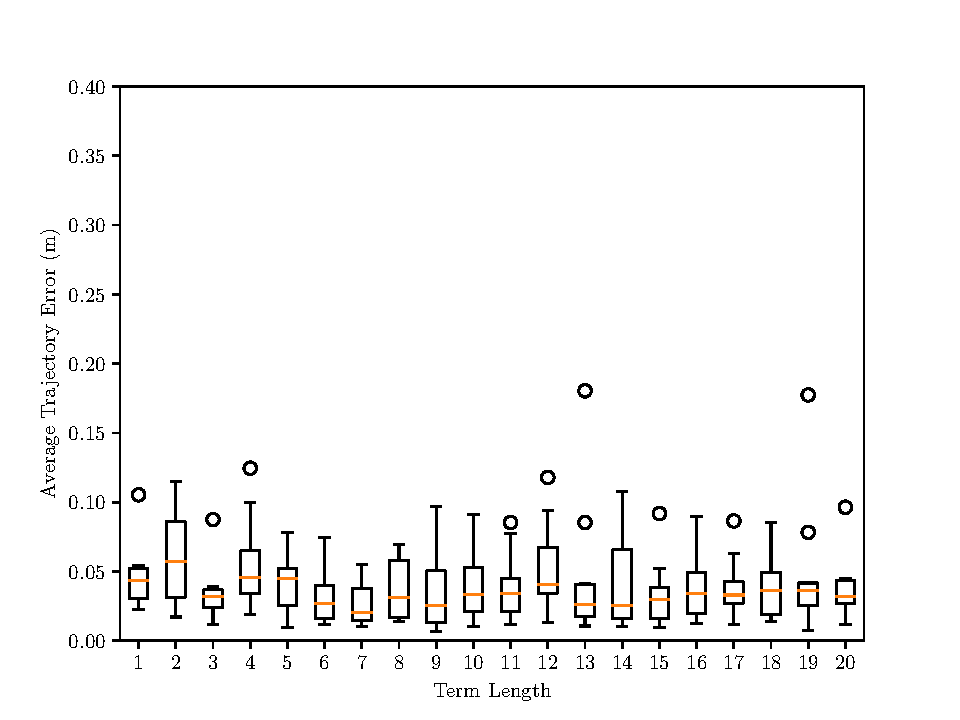
\includegraphics[width=0.3\textwidth]{report/graphs/fixed_term_resistance.pdf}
		\label{fig:fixed-resistance}
	}
	\subfigure[Resilience]{
		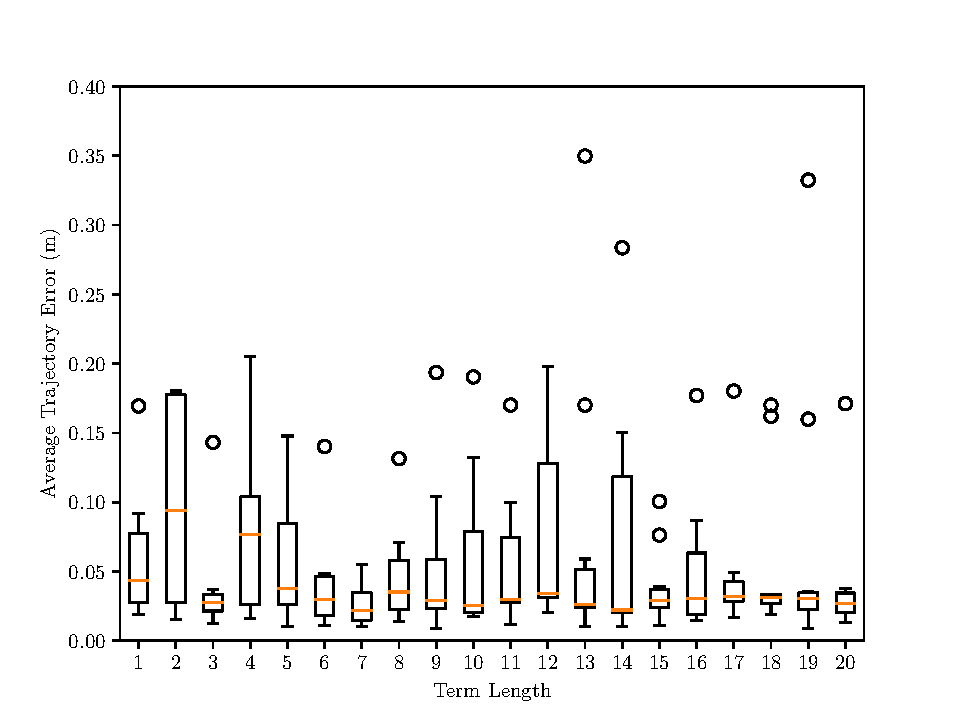
\includegraphics[width=0.3\textwidth]{report/graphs/fixed_term_resilience.pdf}
		\label{fig:fixed-resilience}
	}
 	\subfigure[Cost of Operation]{
		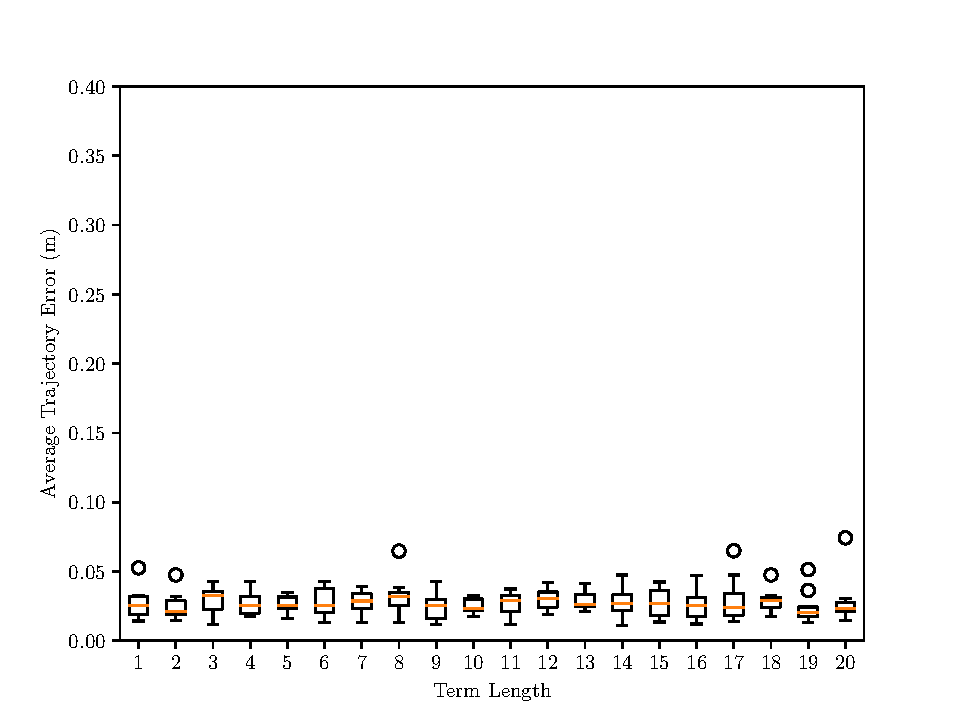
\includegraphics[width=0.3\textwidth]{report/graphs/fixed_term_reduction.pdf}
		\label{fig:fixed-reduction}
	}
	\caption{Finding the optimal length for a FTRP}
        \label{fig:fixed}
\end{figure}

Looking at \autoref{fig:fixed}, we find no correlation between the length of a term and the overall performance of the FTRP. However, this defies our earlier theory, that longer term lengths should result in worse performances. We again suspect that further investigation is required to verify this.

A CBRP is more complex, here a leader will only retire if its confidence in its localisation falls below the threshold $c$. This aims to ensure that leaders will serve for as long as possible before retiring. However, this ``confidence'' value is hard to define, as a robot's confidence is represented by the values in its precision matrix, $\Lambda$, which contains more than 1 value. So to implement CBRP, we must first define the ``confidence'' of a robot. We define it as the smallest eigenvalue of $\Lambda$. We now vary $c$ from 0.0001 to 10, and repeat each experiment 10 times.

\begin{figure}[!h]
	\centering
	\subfigure[Resistance]{
		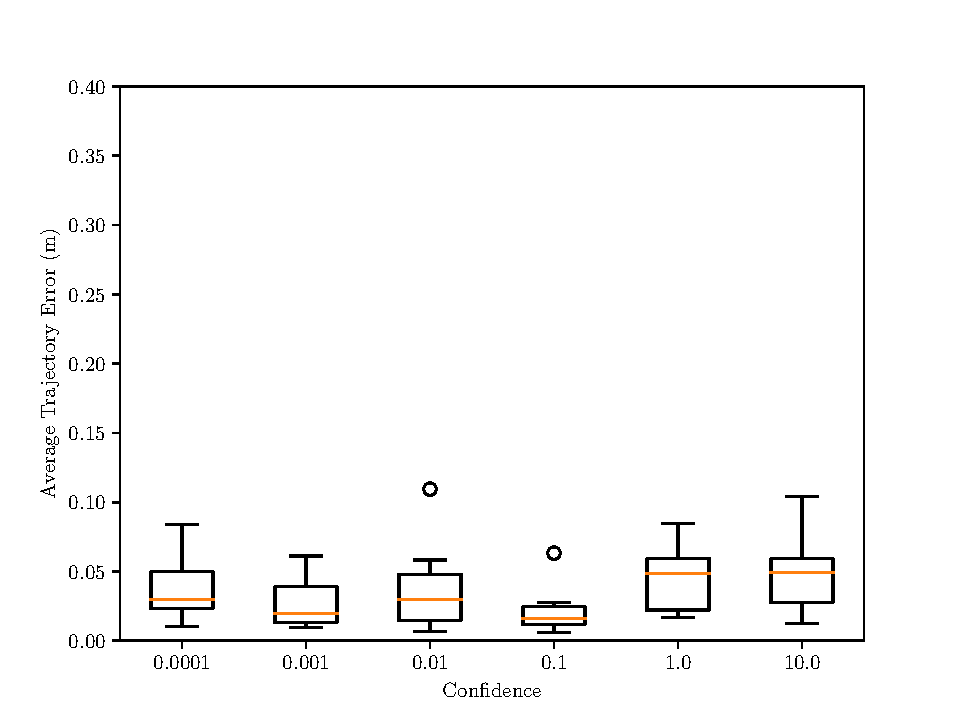
\includegraphics[width=0.3\textwidth]{report/graphs/confidence_based_resistance.pdf}
		\label{fig:conf-resistance}
	}
	\subfigure[Resilience]{
		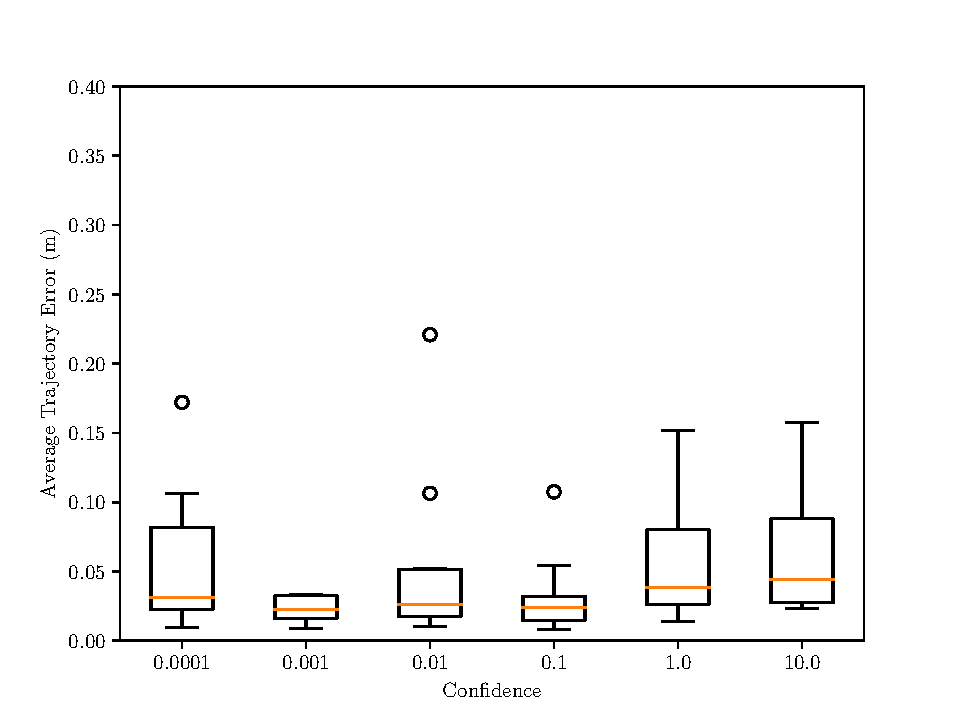
\includegraphics[width=0.3\textwidth]{report/graphs/confidence_based_resilience.pdf}
		\label{fig:conf-resilience}
	}
 	\subfigure[Cost of Operation]{
		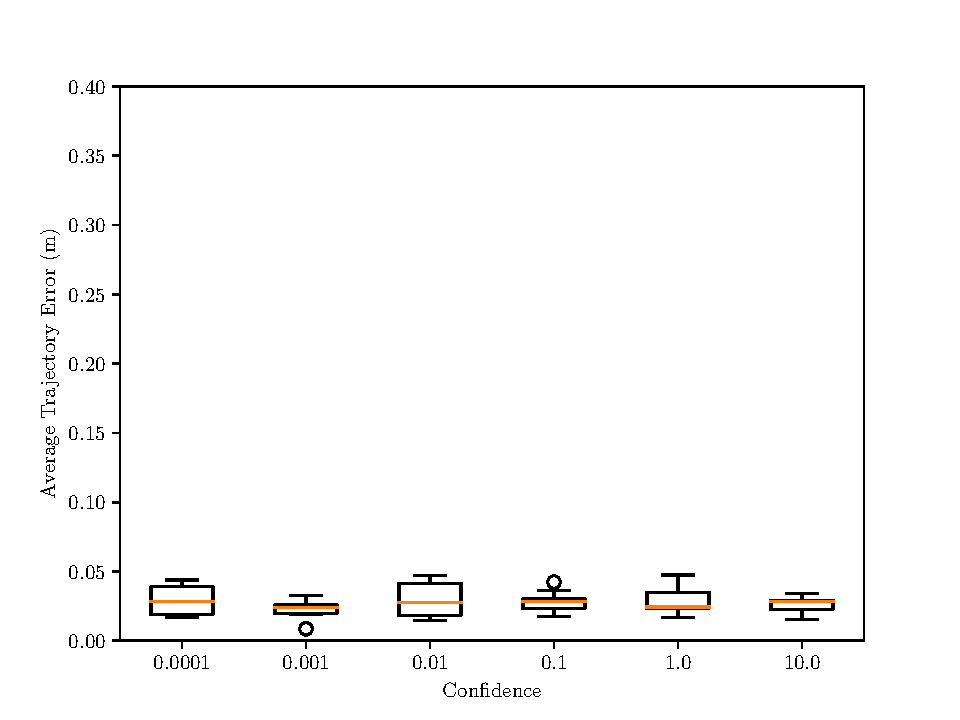
\includegraphics[width=0.3\textwidth]{report/graphs/confidence_based_reduction.pdf}
		\label{fig:conf-reduction}
	}
	\caption{Finding the optimal confidence threshold for a CBRP}
        \label{fig:conf}
\end{figure}

From \autoref{fig:conf}, we can see that the confidence threshold does not have an impact on the resistance, resilience, or cost of operation of Aegis. However, we also see a noticeable improvement in performance across all metrics, which indicates that a CBRP is a more suitable choice. These results also lead us to suspect that the reason why the previous experiments showed no correlation between the length of a leader's term and performance, is because there truly is no correlation between them. However, this remains to be confirmed.

In conclusion, we believe that a CBRP is the best choice of policy and that future work in improving Aegis' policies should use it as a starting point, rather than using any time based retirement policies.

\subsubsection{Comparing different Successor Identification Policies}
We now compare the random successor identification policy with three new ones - a Least-Recently-Lead (LRL-SIP), a Confidence-Based (CB-SIP), and a Centroid (C-SIP) successor identification policy. Neither of these has any configurable parameters, allowing us to directly compare them without first tuning either.

A LRL-SIP aims to promote fairness, where each robot has an equal opportunity to become a leader. Here a leader will choose the follower who led the longest time ago. This ensures that no robot spends too much time as a follower. However, it makes its decision whilst eschewing the suitability of each potential successor. For example, a robot with lower confidence could be chosen over one with higher confidence, which should prove detrimental to the quality of the entire group's localisations.

A CB-SIP aims to remedy this, by choosing the robot with the highest confidence. Once again, the confidence of a robot is defined as the smallest eigenvalue of its precision matrix, $\Lambda$. However, this approach has a glaring fault - it can allow attackers to gain influence. Since followers are weakly-defended, their confidences can be artificially increased. Now an attacker may ensure that certain robots are chosen, by increasing their confidences. And since attackers are hostile, these are likely to be poor choices. However, the feasibility of this as an attack vector is debatable, as attackers would need to know which robots are leaders and which are followers.

Finally, a C-SIP aims to choose leaders who will serve the most number of robots. A leader following a C-SIP will find the centroid of its known followers, and then choose the follower closest to that centroid. This should ensure that the chosen robot serves as many followers as possible. 

We now compare the performance of each SIP, repeating each experiment 10 times.

\begin{figure}[!h]
	\centering
	\subfigure[Resistance]{
		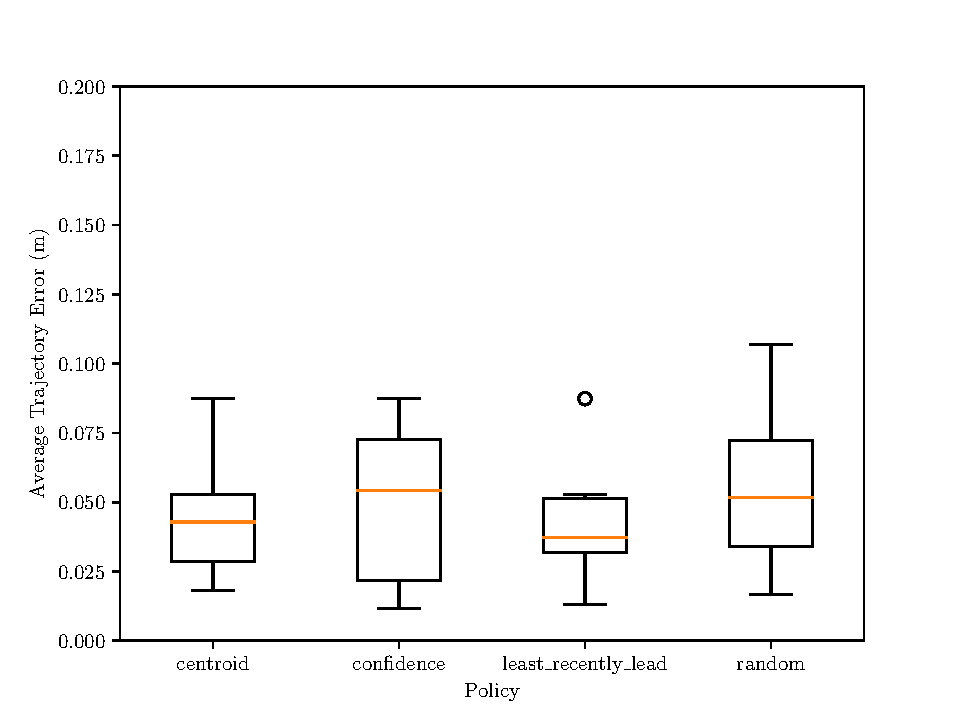
\includegraphics[width=0.3\textwidth]{report/graphs/policy_resistance.pdf}
		\label{fig:policy-resistance}
	}
	\subfigure[Resilience]{
		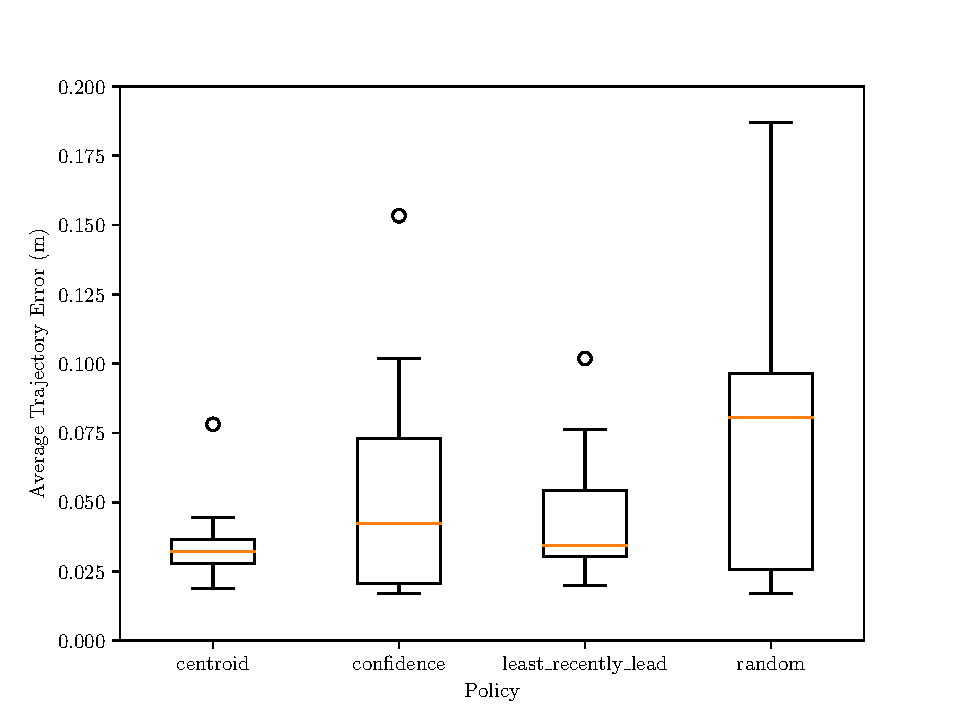
\includegraphics[width=0.3\textwidth]{report/graphs/policy_resilience.pdf}
		\label{fig:policy-resilience}
	}
 	\subfigure[Cost of Operation]{
		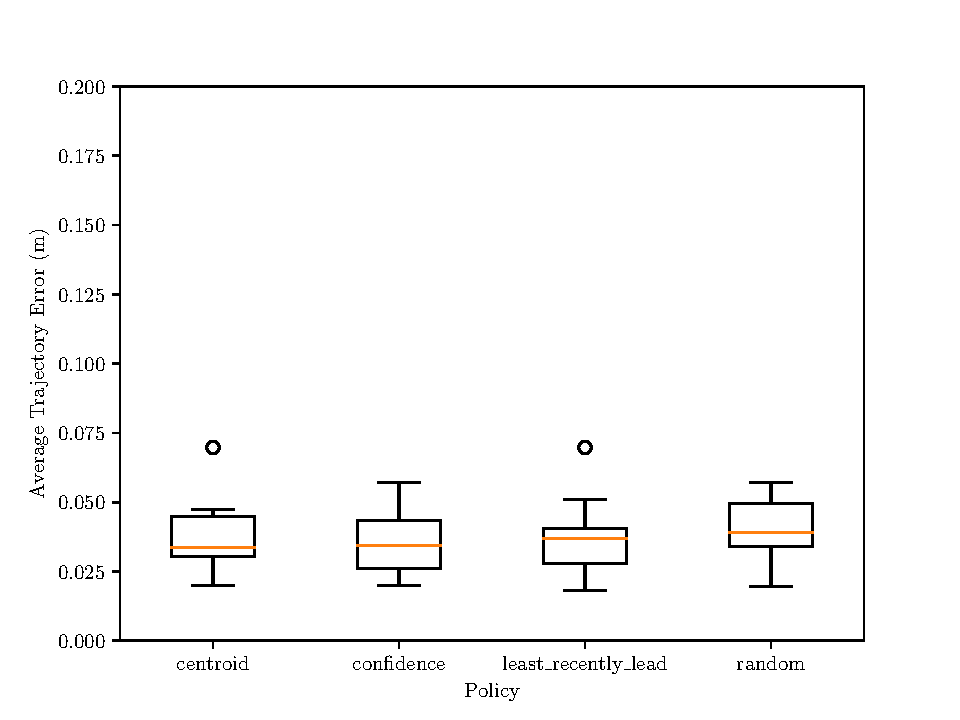
\includegraphics[width=0.3\textwidth]{report/graphs/policy_reduction.pdf}
		\label{fig:policy-reduction}
	}
	\caption{Comparing between a Random, Least-Recently-Lead, Confidence-Based, and Centroid Successor Identification Policy}
        \label{fig:policy}
\end{figure}

Looking at \autoref{fig:policy-resistance}, we see that all four policies have comparable performances when it comes to their ability to resist attacks, yet when we examine \autoref{fig:policy-resilience}, we see that the C-SIP decisively outperforms the others. This effect may be due to the fact that the baseline estimates formed using a central (not centralised) leader are simply more confident than those formed by others. This would occur as the quality of a leader's measurements, decreases as the follower it is measuring moves further from it. Finally looking at the Cost of Operation in \autoref{fig:policy-reduction}, we again see no clear difference between successor identification policies.

\subsubsection{Varying the Permissiveness of Followers}
The permissiveness of a follower refers to how far a message can be from the baseline estimate for it to still be accepted. This variable is represented by the $\epsilon$ (the \textbf{Maximum Leader Divergence}) parameter. We believe that a follower's permissiveness should occupy a ``Goldilocks Zone'' being neither too high nor too low. If a follower is too permissive, then it can be easily exploited by attackers, who would have a large range of localisations to force it to. On the other hand, a follower that is too strict would ignore many helpful messages. This leads us to believe that an optimal level of permissiveness exists.

\begin{figure}
    \centering
    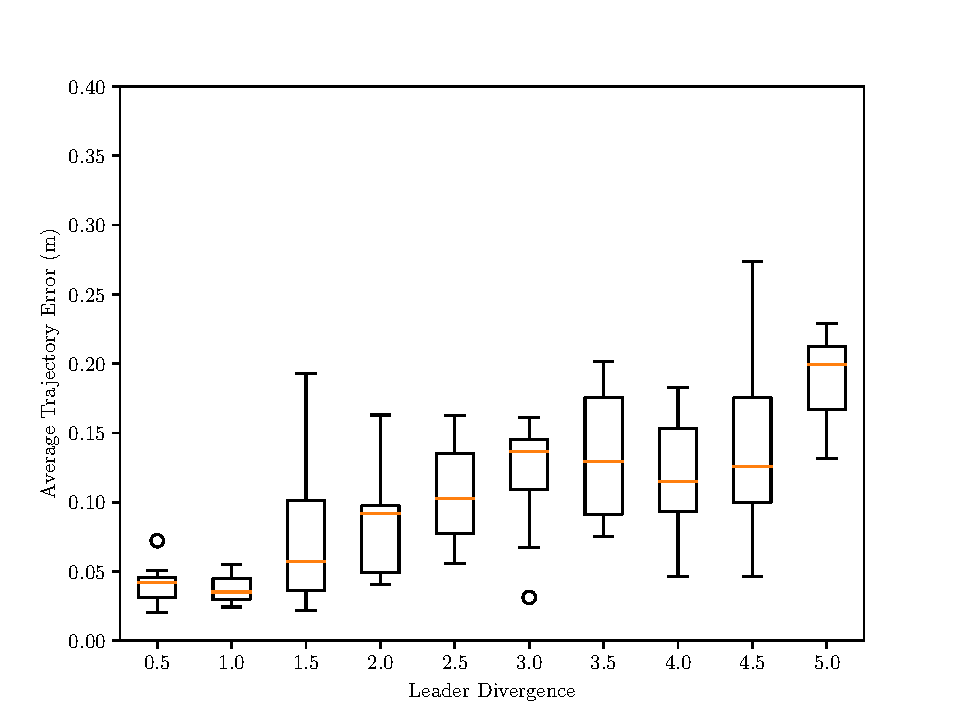
\includegraphics[width=7cm]{report/graphs/leader_divergence_max.pdf}
    \caption{Finding the optimal value $\epsilon$ for the permissiveness of a follower}
    \label{fig:leader-div}
\end{figure}

In \autoref{fig:leader-div} we see a clear trend confirming our hypothesis, as increasing the divergence of a leader subsequently decreases its performance. We also see this effect plateau when $\epsilon$ falls below 1. This plateau is likely caused by the followers only listening to their leaders, rather than one another. In fact, we believe that if this experiment were to be rerun with many robots and many groups, then the effect of this plateau would be more pronounced, as robots further lose their ability to benefit from others.

\subsubsection{Varying the Number of Leaders}
The final parameters we tune are the minimum and maximum numbers of leaders respectfully. We believe that increasing the minimum number of leaders will have a more pronounced effect than increasing the maximum number of leaders. The reason for this is that there \textit{must} be at least $L_{min}$ leaders, but there \textit{can} be upto $L_{max}$ leaders, so increasing $L_{max}$ does not necessarily increase the actual number of leaders in a group. Nevertheless, we believe that increasing the number of leaders will improve the resistance and resilience of a group, whilst simultaneously worsening the cost of operating Aegis.

We now vary $L_{min}$ and $L_{max}$ from 1 to 4, repeating each experiment 10 times.
\begin{figure}[!h]
	\centering
	\subfigure[Resistance]{
		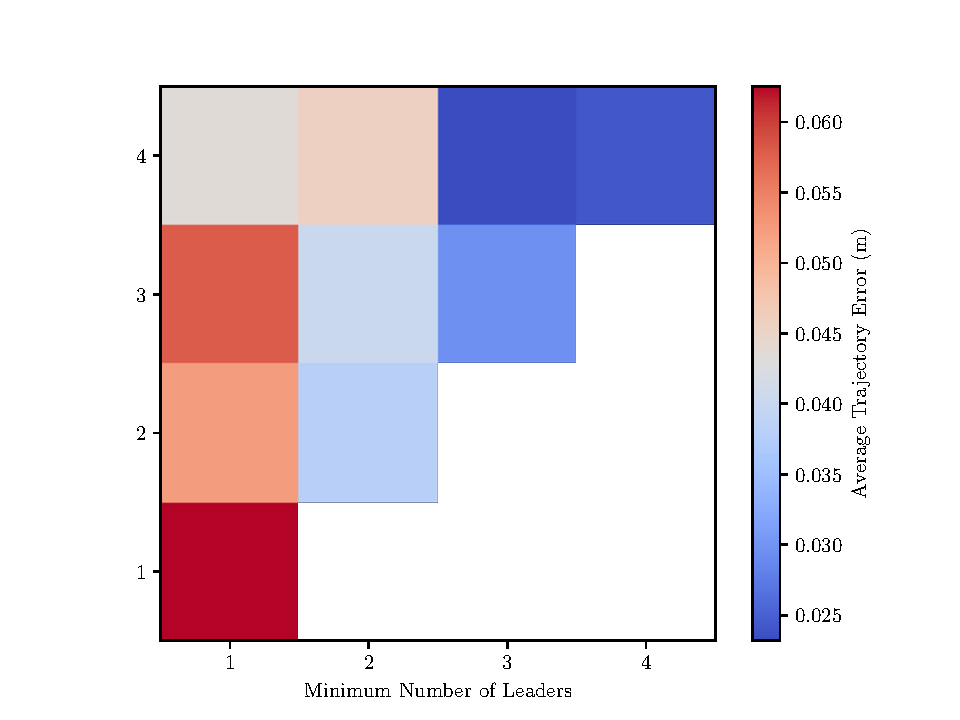
\includegraphics[width=0.3\textwidth]{report/graphs/n_leaders_resistance.pdf}
		\label{fig:n-leaders-resistance}
	}
	\subfigure[Resilience]{
		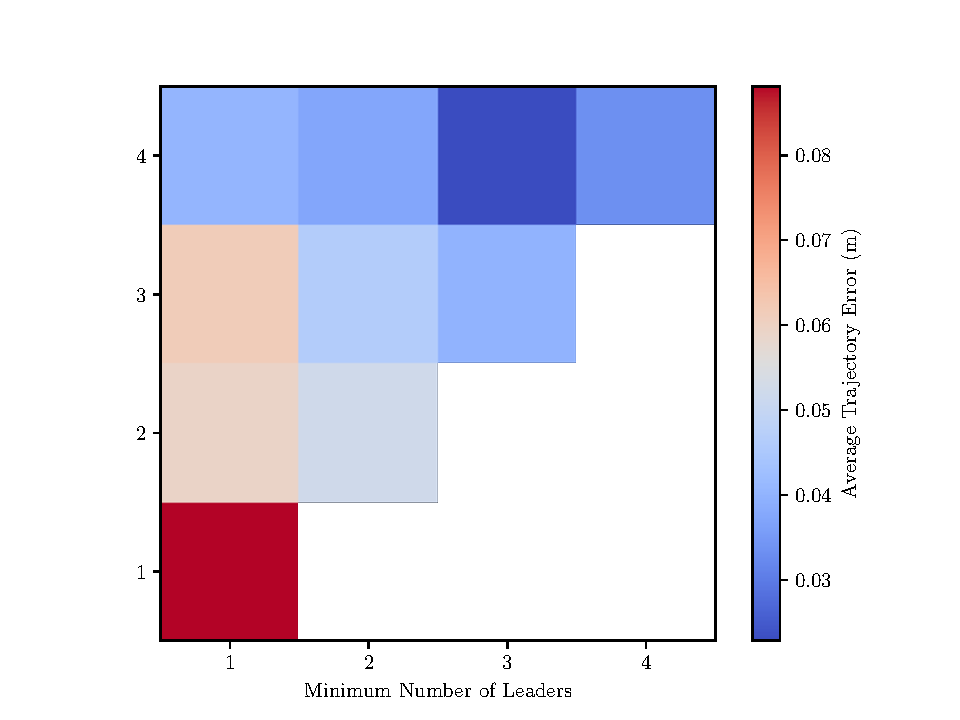
\includegraphics[width=0.3\textwidth]{report/graphs/n_leaders_resilience.pdf}
		\label{fig:n-leaders-resilience}
	}
 	\subfigure[Cost of Operation]{
		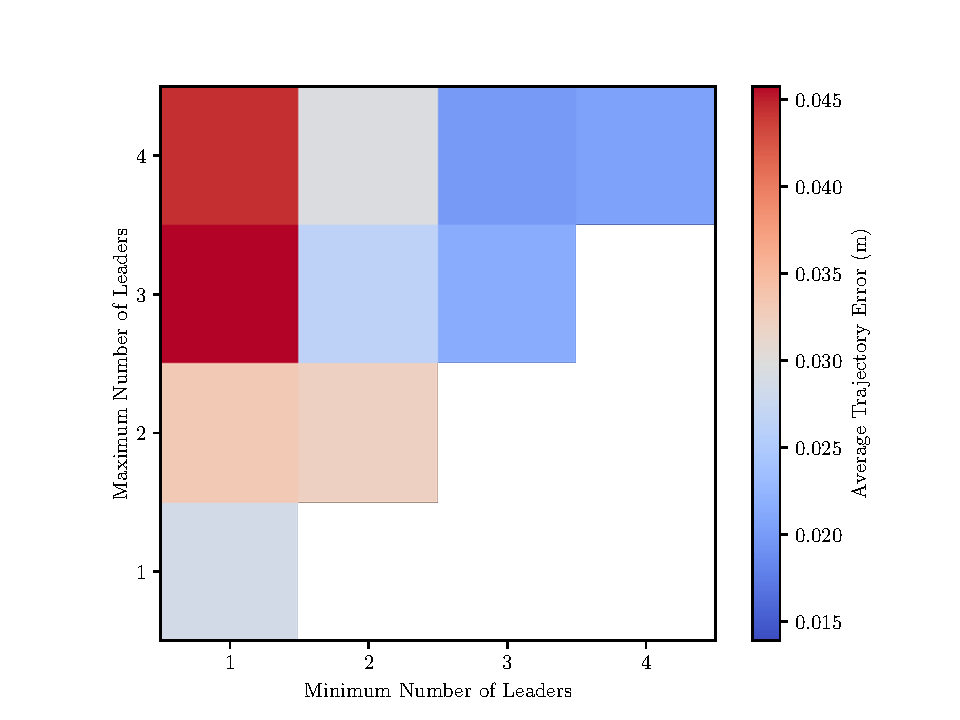
\includegraphics[width=0.3\textwidth]{report/graphs/n_leaders_reduction.pdf}
		\label{fig:n-leaders-reduction}
	}
	\caption{Varying $L_{min}$ and $L_{max}$}
\end{figure}

From \autoref{fig:n-leaders-resistance} and \autoref{fig:n-leaders-resilience}, we can see a marked improvement in performance as both $L_{min}$ and $L_{max}$ increase, notably an increase in $L_{min}$ affects the performance more than one in $L_{max}$, confirming our theory. We also see in \autoref{fig:n-leaders-reduction}, that increasing $L_{max}$ does increase the cost of operation, yet increasing $L_{min}$ does not.
\chapter{Conclusion}

\section{Ethical Considerations}

\begin{quote}
    \centering 
    ``A new device merely opens a door; it does not compel one to enter''\\
    \attrib{Lynn White \cite{MedievalTechnology}}
\end{quote}

From the discovery of coffee leading to the ``Age of Enlightenment'' to the invention of Boolean algebra creating our modern digital age, history has repeatedly shown us that it is impossible to fully understand the implications of new discoveries and nascent technology. With this in mind, we provide a short discussion of potential ethical issues which, we believe, may arise as a consequence of the research conducted in this thesis.

As with all research enabling autonomous robotics, we must consider potential military applications. Many militaries today already use unmanned aerial combat vehicles in their operations, if they were to incorporate this research, they may be able to improve their performance by allowing them to share information securely. However, we do not believe that this is likely to occur as militaries tend to have highly centralised structures, where each robot would have prior knowledge about other trusted robots in the network. Whereas our research focuses on providing security to untrusted robots in decentralised networks.

Another potential misuse of this research would be enhancing the capabilities and security of surveillance robots. In this scenario, an authoritarian regime would use robots to continuously monitor their citizens. The robots would communicate with others in their immediate surroundings to coordinate their search and could be vulnerable to cyber attacks where several are hijacked. The hijacked robots would then send incorrect messages to prevent certain areas from being searched. However, it is unlikely that this research would be an ideal candidate for implementing such a dystopia, as a single party would own the robots and would find it much simpler to implement centralised security measures.

Alongside the unethical misuses of this research, there exist several scenarios where it would confound unethical groups. One intended use case is to implement a common robotic infrastructure for autonomous robots owned by many different parties. Here the decentralised nature of the infrastructure would provide asymmetric robustness against hackers or governments seeking to unilaterally disrupt and destroy the infrastructure as they would not be a single point of failure.

In conclusion, there are many scenarios where this research may be misused to the detriment of humanity, yet we are not convinced that this research would be the most appropriate in those examples. Furthermore, given how this research seeks to defend against bad actors, we believe it is more likely to be a benefit to humanity.
% \appendix
\chapter{First Appendix}

\bibliographystyle{vancouver}
\bibliography{report/bibs/sample}
\addcontentsline{toc}{chapter}{Bibliography}

\end{document}